

\section{红楼梦}


\par 红楼梦:全三册
\par 作者:(清)曹雪芹著;(清)无名氏续;(清)程伟元,(清)高鹗整理;中国艺术研究院红楼梦研究所校注.—3版
\par 出版社:人民文学出版社
\par 版本:1982年3月北京第1版,2008年7月北京第3版;2020年6月第2次印刷
\par 书号:978-7-02-016117-1

\subsection*{《红楼梦》校注本三版序言}

\par 本书初版于一九八二年,至今忽忽已历二十五周年,发行量已逾三百五十万套。一九九四年,当此书面世十二年的时候,我们曾修订过一次,改正了初版中的一些疏漏讹误,也吸收了红学研究上的新成果。现在距离上一次的修订,又已过了十三个年头。红学是一门最具群众性的学问,它拥有的研究队伍和读者,可能远比其他学科的人数要多得多。这十三年的过程,在红学的研究上,自然又有很多的收获,因此,我们决定再次进行修订。
\par 记得一九七五年校订开始之初,我们曾为选用底本,进行过热烈的争论,最后决定采用乾隆二十五年的庚辰本(指底本的年代)为底本,现在看来,当时的这个选择是正确的。广大读者和研究者接受和认可这个本子就是最好的证明。同时,对庚辰本的研究不断深入,而且一九九四年齐鲁书社又出版了同样以庚辰本为底本而又汇集脂评的校订本,到二〇〇六年,作家出版社又出版了一种庚辰本的校订本,这说明庚辰本的真正价值,日益为学术界所认识了。我们作为首次大胆采用庚辰本为底本来校订《红楼梦》的学人,当然是欢迎的。《诗经·小雅·伐木》说:“嘤其鸣矣,求其友声。”这种学术上的求同之心,是大家可以理解的。
\par 我们注意到,新出的以庚辰本为底本的校本,尤其是二〇〇六年的作家本,大量采用了我们的校订成果,这是值得欢迎的。当时我们遵国务院古籍整理组组长李一氓先生之嘱,校记要精,只有重要的改动才作校记。这样做,一方面是为了方便读者的阅读,避免繁琐;另方面,也是为了降低书的定价,有利于读者购买。所以我们大量校改的文字并未出校记。遗憾的是,作家本的校者,并不说明他的校本上的校文,基本上是用了前人的成果,他把这些校文用黑体字排出,还在《校勘说明》里明确说:“补改文字,一律用黑体,使之和原抄文字相区别,便于读者区分与比较。”这段话分明就是告诉读者,这些用黑体字排的文字,全是他新校出来的。而实际上这些用黑体字排的校文,有百分之九十以上是我们早就校出来的。这只要用人民文学出版社出版、中国艺术研究院红楼梦研究所的校订本一对就明白了。
\par 我们的校订本,距今已二十五年了,当时用了七年时间才完成了这项任务。现在有的同志同样采用庚辰本作底本,大量采用我们的校文,这足以说明当时对底本的选择和校订文字的斟酌去取,是经得起时间的考验的,也为后来的校订者起了铺路的作用。
\par 学无止境,学问是与时推移,日新月异的,红学也是一样。所以我们这次的校订,参阅了近十多年来的多种新校本和红学论著,自觉收获较大。这些收获,当然不是个人的,而是反映了红学研究的成果,应该看作是红学界的共同成果。
\par 这次校订,计正文修订共五百馀条,校记修订共一百馀条,注释修订共三百馀条,其中增加条目二百馀条;修改条目一百馀条;凡例修订共三条。
\par 以上是这次修订的总情况。
\par 这次校订,校和注两方面都有相当的进展,这些都已包含在书里,不再一一列举。
\par 这次参加校订工作的人手较少,主要是冯其庸和胡文彬、吕启祥、林冠夫四个人。冯其庸同志负责正文的校订,吕启祥同志负责注释的修订和增补,胡文彬同志正文和注释两方面的工作都参加,并且由他来承担校和注两方面的合成工作,林冠夫同志,考虑到他的身体,主要是请他参加讨论和商量去取。胡文彬同志合成后,最后由冯其庸同志统一审阅和修改定稿。由于第一道工序校和注都做得很认真,所以校注两方面的修改面和难度虽然较大,但质量却比以往有所提高。胡文彬同志的合成工作,负担很重,文字量也大,但做得非常认真细致。尽管恰值酷暑,我们还是尽心尽力尽快地完成了预期的工作任务。
\par 当然,在这项工作启动以前,原校订组的副组长李希凡同志和我们四人,还有人民文学出版社的有关领导曾一起开会商量确定这项工程,之后还分别取得了散处在各地的原校订组成员的同意。这也是促使我们四个人加紧努力的因素。
\par 这里特别要谢谢陈熙中教授,他应我们的邀请,为我们写了几十条修订意见,都十分可贵。还有老友黄能馥老先生,重新为我们审定修改了有关服饰方面的注释,安徽的老友周中明教授,应我们的邀请,花了整整两个月的时间,为我们检核全书,写出了不少关于通假字、同音字厘定的意见和正文校补的意见。由于以上几位同志的帮助,使本书的校订,较前更有所提高。
\par 在整个校订过程中,任晓辉同志协助我们做了许多诸如查阅资料,复印稿件,递送信息等等的工作,使得这项工作得以快速有效的运转。
\par 本书自初版以来,不断收到各地热心的红学朋友的来信来稿,有的是热情鼓励,有的是指出错误,对我们都有很大的帮助。最近,我们又收到河南新安县冯东先生的来信,他为我们细心地查出了错字、注码误差等等问题。还有河北的一位红友萧凤芝同志,他来信告诉我们《红楼梦》第四十七回庚辰本作“十月一”是对的。这是北方为已故亲人送寒衣的民俗节日,不能改作“十月初一”。我们请教了周围的老北京人和北方的朋友,都说至今仍有“十月一,送寒衣”的民俗,所以我们仍依庚辰原本作“十月一”。在此我们敬向以往所有在报刊上发表文章指谬商榷和来信来电的读者朋友表示衷心的感谢!
\par 凡此,都说明,《红楼梦》的研究和校订,既离不开红学研究者,也离不开广大读者。《红楼梦》的修订工作,不会到此结束。我们希望今后能继续走专家和群众结合的路线,实事求是地将这部名著整理得更为完善。
\par \rightline{红楼梦校注组}
\par \rightline{二〇〇七年八月十三日}
\par 本书自二〇〇八年第三版至今,忽忽又将五载。在此期间,承广大读者和学界同仁关切,我们亦时时自省自检,发现仍存在若干疏漏和个别修改失当之处,包括印制过程中的失校。为了对读者负责,今年初,在冯其庸先生建议和主导下,对全书再做修订,具体操作悉委胡文彬、吕启祥二位,仍由胡文彬汇总,计改动正文及标点四十六处、注释十六处。馀者技术性的改动均归责任编辑徐文凯同志。
\par 此次小的改动乃属第三版即同一版次中的修葺。我们深知校书如扫落叶、注释如爬高坡,无有止境。在力所能及的范围内使本书减少讹误、趋向完善,是我们的真诚愿望。
\par 是为记。
\par \rightline{红楼梦校注组}
\par \rightline{二〇一三年四月}

\clearpage
\subsection*{《红楼梦》校注本再版序}
\begin{center}
    \par 冯其庸
\end{center}
\par 本书初版于一九八二年三月,距今转瞬已十二年。本书初版以来,受到广大读者和专家们的欢迎,也得到了不少指正。
\par 这十二年的岁月,使我们进一步认识到,我们当时确定的几个原则是正确的:一是我们所选择的底本——庚辰本,确是一个学术价值很高、接近曹雪芹原稿的珍贵本子,我们以此为底本,就使这个校本有了很好的基础;二是我们确定的校勘原则(详见《校注凡例》)也是正确的,这样就使我们的校勘工作做到了审慎和准确,不至于随意改动底本文字,从而较好地保持了原本的历史面貌;三是我们确定的注释原则(见《校注凡例》)也是切合实际的,对象适中,繁简得宜,因而使得本书避免臃肿烦琐之病。
\par 但是,学问是无止境的,“红学”更是日新月异,这十多年来“红学”研究已有了长足的进展,不少重要的专著相继出版了,不少重要的论文陆续发表了,还连续发现了有关曹雪芹家世的文献和实物。在《红楼梦》的名物考订上,也有不少的进展。对照我们的校本,就感到有了历史的差距。为了对读者负责,对我们的“红学”事业负责,我们深深感到有对本书作一次全面修订的必要。于是趁此书再版之机,我们就着手这一新的繁重工作。
\par 此书初版是由《红楼梦》校订组先作出初稿,然后由校订组和注释组反复修改定稿的,其详细情况见初版的《前言》。现在全面重新整理、重新校注时,不可能把原有的人都邀请回来了,幸好初版定稿时的三位同志:冯其庸、林冠夫、吕启祥都还在原工作岗位上,因此本次的校注,即由他们三位负责:由冯其庸总负其责,林、吕二位分别作校、注的具体修订工作。
\par 关于注释的修改和增补,计新增注释八十七条,补充和修改原注一百六十五条,其馀所有注释,共二千四百零一条,从内容到文字也重新作了一次审核认定;在校勘和标点、分段方面,重校的文字为数亦不在少。特别是此次重校过程中,仍用各脂本仔细复核,所以费力较多;至于标点和分段,则改动更多,不能一一列举。最后,由我作校、注两方面的审核工作,修改核定校、注的条目和文字,以及有关此次重新校注的其他事宜。以上种种,无法一一详述,读者翻阅此再版校注本,当可了然。
\par 尽管此书又作了较为详慎的重校和重注,但初版的创始之功自不可没,故初版的《前言》、《校注凡例》等文字仍置于卷首,以示不忘,也正说明前后校注的原则是一贯的。
\par 这里特别要说明的是,一九七四年至一九七五年间,倡议对《红楼梦》作校注整理,是由袁水拍同志向上级提出的。一九七四年秋天,袁水拍同志到我住处看望我,并提到整理古籍的问题。当时我提及《红楼梦》的校注问题,水拍同志极为重视,不久就要我草拟一个报告。此事后经国务院有关部门正式批准,由水拍同志任校注组的组长,由我和李希凡任副组长。初期校勘的稿子(即内部用的大字本),水拍同志还认真看过,凡是他不理解的地方,他还都提出来认真地询问过。后来,他因事因病,不再过问此事,但在重病中,仍希望能看到此书的出版。所以《红楼梦》的新校注工作得以正式立项并由政府拨款,调集一批专家和研究人员来工作,水拍同志是起了倡导推动作用的。现在水拍同志已经作古十年,当着此书修订再版的时候,我有责任将此经过叙明,亦以慰逝者于地下。
\par 时间虽然只过了十二年,但参加此书工作的同志,却已经作古了好多位,其中顾问有:叶圣陶、吴世昌、吴恩裕、吴组缃先生。参加校注工作的有:沈彭年、陶建基、徐贻庭、朱彤、祝肇年、江辛眉、杨廷福诸先生。国务院古籍整理组组长李一氓先生,一直关心《红楼梦》的研究工作,此书出版后,他还亲自写过评论文章,热情地肯定了这个新校注本,但李一氓先生也已经不幸逝世了。对以上十二位已故的先生和朋友,我们只能寄以哀思,以志永怀!
\par 此次修订再版,虽然由我们三人负责,但前人之功不可没,而“红学”方兴未艾,且无止境,故以后的校注工作,亦无有止境。故我们本次的修订,只是万里长途中的一站,瞻望前途,曷其有极!惟愿再奋馀勇,更求寸进,并望“红学”同人和专家读者进而教之,则《红》书幸甚!“红学”幸甚!
\par 是为序。
\par \rightline{一九九四年七月六日于京华宽堂}

\clearpage
\subsection*{前言}


\par 曹雪芹,是中国文学史上最伟大也是最复杂的作家,《红楼梦》也是中国文学史上最伟大而又最复杂的作品。
\par 关于曹雪芹,目前还存在着不少有争论的问题,不仅他的生卒年一直存在着争议,甚至连他的“字”、“号”也不能十分确定,按照曹雪芹的好友张宜泉的说法,应该是“姓曹名霑,字梦阮,号芹溪居士”,但有的研究者认为他的“字”是“芹圃”,号“雪芹”。
\par 他的生卒年问题,已经争论了几十年。他的生年,现在主要的有两种看法,一种认为他生于公元一七一五年,即康熙五十四年乙未;另一种说法认为他生于公元一七二四年,即雍正二年甲辰。他的卒年,主要有三种看法,一种认为他卒于公元一七六三年,即乾隆二十七年壬午除夕;另一种说法认为他卒于公元一七六四年,即乾隆二十八年癸未除夕;还有一种说法认为他卒于公元一七六四年初春,即乾隆二十九年甲申岁首\footnote{按乾隆二十八年除夕,已经是西历一七六四年二月一日,故乾隆二十九年甲申仍为一七六四年。}。现在大都倾向于第一种看法。
\par 曹雪芹的父亲,现在也有两种看法。一种认为是曹颙,曹雪芹是他的遗腹子;另一种看法,则认为是曹頫。
\par 曹雪芹的上世的籍贯,据近三十年来发现的大量可靠史料,证明他的祖籍是辽阳,后迁沈阳,他的上祖曹振彦原是明代驻守辽东的下级军官,大约于天命六年后金攻下辽阳时归附,以后随清兵入关。\footnote{周汝昌、杨向奎先生认为曹雪芹祖籍是河北丰润,但这是没有任何根据的臆想,是不可信的。详见冯其庸著《曹雪芹家世新考》(上海古籍出版社1980年版)、《再论曹雪芹的家世、祖籍和〈红楼梦〉的著作权》(《红楼梦学刊》1995年第1期)。}
\par 曹振彦归附后金以后,先是属佟养性管辖,后来又归了多尔衮属下的满洲正白旗,当了佐领。旋即跟随清兵入关。曹振彦在入关前的明、金战争中以及入关后的平姜瓖之叛的战争中是立过功的,他历任过山西吉州知州、阳和府知府、浙江盐法道等官职。曹家的发迹,实是从曹振彦开始的。此后,曹振彦之媳,即曹玺之妻孙氏当了康熙的保母。康熙二年,曹玺首任江宁织造之职,专差久任,至二十三年在江宁织造任上病故,康熙旋即命其子曹寅任苏州织造,后又继任江宁织造、两淮巡盐御史等职,并命其纂刻《全唐诗》、《佩文韵府》等书于扬州。曹寅很得康熙的信任和赏识,康熙南巡时曾主持过四次接驾大典。康熙五十一年曹寅在扬州任上病危,康熙特命快马送药抢救,曹寅病故后,又特命其子曹颙继任江宁织造。康熙五十三年曹颙病故,康熙又特命曹寅的胞弟曹荃(宣)之子曹頫过继给曹寅并继任织造之职,直至雍正五年十二月二十四日曹頫被抄家败落,曹家在江南祖孙三代先后共历六十馀年。
\par 《红楼梦》的作者伟大作家曹雪芹就是出生在南京的。直到雍正六年曹家抄没后才全家迁回北京。当时,曹雪芹尚年幼,按生于乙未说是虚岁十四岁,按生于甲辰说是虚岁才五岁。曹家回北京以后的情况,文献绝少记载,曹頫曾经在给康熙的奏折里说到“惟京中住房二所,外城鲜鱼口空房一所;通州典地六百亩,张家湾当铺一所,本银七千两”\footnote{《关于江宁织造曹家档案史料》132页。}等等。在曹家被抄以后,隋赫德的报告里也说到:“曹頫家属,蒙恩谕少留房屋,以资养赡,今其家属不久回京,奴才应将在京房屋人口,酌量拨给。”\footnote{《关于江宁织造曹家档案史料》188页。}据近年发现的雍正六年六月二十一日《曹頫骚扰驿站获罪结案题本》及雍正七年七月《刑部移会》,得知曹頫抄家前,尚有骚扰驿站案,并于雍正六年结案,曹頫被枷号催追赔款。雍正七年七月,曹頫尚在枷号中。又据《刑部移会》得知曹家尚有“京城崇文门外蒜市口地方房十七间半,家仆三对,给与曹寅之妻孀妇度命”。但以后情况究竟如何?究竟拨给了哪些房子?曹雪芹究竟住在何处?他的青年时期是如何度过的?这些问题,统因文献无征,不能确指。据红学家们的考证,认为他与敦诚、敦敏成为亲密朋友,是在右翼宗学里开始结识的,后来落魄住到了西郊,他的不朽的巨著《石头记》就是在西郊的山村里写成的。
\par 曹雪芹晚年的生活穷愁潦倒而又嗜酒狂放,朋友们常把他比作晋朝的阮籍。他甚至穷困到“举家食粥”的地步,常常要靠卖画来换酒喝。他的画很为当时的朋友们所推重。敦敏《题芹圃画石》诗说:“傲骨如君世已奇,嶙峋更见此支离;醉馀奋扫如椽笔,写出胸中磈礧时!”可见曹雪芹的胸襟和画风。可惜他的遗作至今尚未发现。
\par 伟大作家曹雪芹,终于在穷愁困顿中于公元一七六三年即乾隆二十七年壬午除夕去世。他的不朽巨著《石头记》的前八十回,早在他去世前十年左右就已经传抄问世;书的后半部分据专家们研究,认为基本上已经完成,只是由于某种原因未能传抄行世,后来终于迷失,这是不可弥补的损失。
\par 《红楼梦》是一部具有高度思想性和高度艺术性的伟大作品,从本书反映的思想倾向来看,作者具有初步的民主主义思想,他对现实社会包括宫廷及官场的黑暗,封建贵族阶级及其家庭的腐朽,封建的科举制度、婚姻制度、奴婢制度、等级制度,以及与此相适应的社会统治思想即孔孟之道和程朱理学、社会道德观念等等,都进行了深刻的批判并且提出了朦胧的带有初步民主主义性质的理想和主张。这些理想和主张正是当时正在滋长的资本主义经济萌芽因素的曲折反映。
\par 《红楼梦》塑造了众多的人物形象,他们各自具有自己独特而鲜明的个性特征,成为不朽的艺术典型,在中国文学史和世界文学史上永远放射着奇光异彩。
\par 《红楼梦》的情节结构,在以往传统小说的基础上,也有了新的重大的突破。它改变了以往如《水浒传》、《西游记》等一类长篇小说情节和人物单线发展的特点,创造了一个宏大完整而又自然的艺术结构,使众多的人物活动于同一空间和时间,并且使情节的推移也具有整体性,表现出作者卓越的艺术才思。
\par 《红楼梦》的语言艺术成就,更是代表了我国古典小说语言艺术的高峰。作者往往只需用三言两语,就可以勾画出一个活生生的具有鲜明的个性特征的形象;作者笔下每一个典型形象的语言,都具有自己独特的个性,从而使读者仅仅凭借这些语言就可以判别人物。作者的叙述语言,也具有高度的艺术表现力,包括小说里的诗词曲赋,不仅能与小说的叙事融成一体,而且这些诗词的创作也能为塑造典型性格服务,做到了“诗如其人”——切合小说中人物的身份口气。
\par 由于以上各方面的卓越的成就,因而使《红楼梦》无论是在思想内容上或是艺术技巧上都具有自己崭新的面貌,具有永久的艺术魅力,使它足以卓立于世界文学之林而毫无逊色。
\par 现存《红楼梦》的后四十回,是程伟元和高鹗在公元一七九一年即乾隆五十六年辛亥和公元一七九二年即乾隆五十七年壬子先后以木活字排印行世的,其所据底本旧说以为是高鹗的续作,据近年来的研究,高续之说尚有可疑,要之非雪芹原著,而续作者为谁,则尚待探究。续书无论思想或艺术较之原著,已大相悬殊,然与同时或后起的续书相比,则自有其存在之价值,故至今仍能附原著以传。
\par 《红楼梦》在乾隆中叶以后,带脂砚斋评的八十回抄本日多,乾隆末叶即可公开在庙市中抄卖,并且价昂至数十金一部。今传乾隆时期的《石头记》抄本,尚有十一种之多,计有:己卯本、庚辰本、甲戌本、《红楼梦稿》本、蒙古王府本、戚蓼生序本、南京图书馆藏本、梦觉主人序本、舒元炜序本、郑振铎藏本、苏联列宁格勒亚洲图书馆藏本等\footnote{原苏联列宁格勒亚洲图书馆藏本,以往均称列藏本。今因该图书馆已更名为圣彼得堡俄罗斯科学院东方古籍文献研究所,故此书统称俄藏本。特予说明。}。另有南京靖应鹍藏本,今已遗失,又程甲本的前八十回底本,原也是抄本,如果一并计入,则可以说现知的抄本已有十三种之多。当然上面所说的己卯本、庚辰本、甲戌本等名称,其干支年代,都不能代表现有这些本子的抄定年代,都只能表明它们的底本的年代,这一点早已为红学家们指出了。
\par 在以上这些抄本中,己卯、庚辰、甲戌的底本是比较早的。其中己卯本已确知为怡亲王府抄本,其抄成年代约在公元一七六〇年即乾隆二十五年庚辰以后,现存庚辰本抄定的年代,大约是在公元一七六一年即乾隆二十六年以后,甲戌本底本的年代应是公元一七五四年,即乾隆十九年甲戌,但现在所传甲戌本的抄成年代,则是比较晚的。在上述这些抄本中,庚辰本是抄得较早而又比较完整的唯一的一种,它虽然存在着少量的残缺,但却保存了原稿的面貌,未经后人修饰增补(其六十四、六十七两回的残缺,各本皆然,现存各本的这两回或是据程本,或是经后人增补过的),因此本书在校勘过程中决定采用庚辰本为底本,以其他各种脂评抄本为主要参校本,以程本及其他早期刻本为参考本。凡底本文字可通而主要参校本虽有异文但并不见长者,仍依底本;凡底本明显错误而主要参校本不误者,即依主要参校本;凡底本脱漏之文字,有主要参校本可资校补者,即依主要参校本补齐。
\par 本书的注释,凡一应典章制度名物典故以及难解之语词,一般均尽可能作注释,但由于我们的能力有限,而《红楼梦》的注释又极为繁难,因此我们的注不仅可能挂一漏万,而且也可能注释得不尽恰当;我们的校订也同样是如此。有关校订和注释方面的具体情况,均见本书《校注凡例》,这里不再一一详述。
\par 本书校注工作开始于一九七五年,其间参加工作的人员陆续有所更替,工作时间亦长短不一,难以一一表明,现以参加时间先后和姓氏笔划为序,计参加本书校注工作的有:冯其庸、李希凡、刘梦溪、吕启祥、孙逊、沈天佑、沈彭年、应必诚、周雷、林冠夫、胡文彬、曾扬华、顾平旦、陶建基、徐贻庭、朱彤、张锦池、蔡义江、祝肇年、丁维忠。
\par 参加本书最后修改定稿的,校勘方面有:冯其庸、林冠夫、徐贻庭。由冯其庸负责。注释方面有:陶建基、吕启祥、朱彤、张锦池、丁维忠。由陶建基负责。
\par 全书的校注工作由冯其庸同志总负责。
\par 吴世昌、吴恩裕、吴组缃、周汝昌、启功等几位老红学家担任本书校注工作的顾问。
\par 叶圣陶老先生和叶至善同志对本书的校点和注释提了不少宝贵的意见,本书的前半部分,叶圣老还亲自标点、修改过不少地方。为本书的校注提过不少修改意见和撰写过许多条目及注文的还有王雪苔、江辛眉、朱家溍、巫君玉、杨廷福、杨乃济等同志。此外还有不少同志对本书的校注提过宝贵意见或帮助修改过注文,这里限于篇幅,无法一一列出。实际上本书的校注工作是在全国广大群众的热情支持下,是在他们作出的丰硕成果的基础上进行的。
\par 我所的行政工作人员和资料室的同志,也为本书的校注做了不少工作。
\par 南京图书馆对本书的注释和校订曾多次提出书面的修改意见,其他如中国人民大学、北京大学、北京师范大学、北京师范学院、复旦大学、上海师范学院、中山大学、安徽师范大学、哈尔滨师范大学、杭州大学、中央戏剧学院等单位,都给予了热情的支持,我院戏曲研究所和美术研究所、音乐研究所在涉及有关专业方面的问题上,也给予了我们不少指导和帮助。
\par 北京图书馆、北京大学图书馆、中国社会科学院文学研究所图书馆、中国科学院图书馆、南京图书馆、人民文学出版社资料室,为我们提供了许多重要版本和资料。我院的图书馆,则为我们提供了全部的基本参考图书并给予了种种方便和支持。
\par 本书的责任编辑、人民文学出版社古典文学编辑室的王思宇同志对本书的校和注,都提供了许多宝贵的修改意见,付出了不少精力。
\par 本书的校注工作,自始至终,一直是在中国艺术研究院党委和院领导的热情支持下进行的。本院其他行政部门也给我们以多方面的协助,使这项工作得以顺利进行。
\par 对于以上给予本书的校注以大力支持的同志和单位,我们表示衷心的感谢。
\par 本书的校和注,一定还存在着许多缺点,我们衷心期望得到国内外的读者和专家的指正,以便不断修订。
\par \rightline{中国艺术研究院红楼梦研究所}
\par \rightline{一九八一年五月二十日}
\par 一九九四年七月改定关于曹雪芹的祖籍、家世和卒年部分。 冯其庸。 一九九四年七月七日雨窗。

\clearpage
\subsection*{校注凡例}


\par 关于校勘方面:
\par 一、本书以《脂砚斋重评石头记(庚辰〔一七六〇年〕秋月定本)》(简称庚辰本)为底本。底本若干处缺文均依其他脂本或程本补齐,第六十四、六十七回缺文,则采用程甲本补配。
\par 二、以下列各脂评本、抄本及程甲、乙本为参校本:
\par (一)清乾隆甲戌(一七五四年)脂砚斋重评本(简称甲戌本)。
\par (二)乾隆己卯(一七五九年)冬月脂砚斋四阅评本(简称己卯本)。
\par (三)蒙古王府本(简称蒙府本)。
\par (四)戚蓼生序有正书局石印本(简称戚序本)。
\par (五)戚蓼生序南京图书馆藏本(简称戚宁本。此本与戚序本为同一祖本,唯个别处有异。校记中凡未特别列出戚宁异文者,即与戚序本同)。
\par (六)乾隆甲辰(一七八四年)梦觉主人序本(简称甲辰本)。
\par (七)乾隆己酉(一七八九年)舒元炜序本(简称舒序本)。
\par (八)郑振铎藏本(简称郑藏本)。
\par (九)《红楼梦》稿本(简称梦稿本)。
\par (十)圣彼得堡俄罗斯科学院东方古籍文献研究所藏《石头记》(简称俄藏本)。
\par (十一)《卞藏脂本红楼梦》(简称卞藏本)。
\par (十二)乾隆辛亥(一七九一年)程伟元初排活字本(简称程甲本)。
\par (十三)乾隆壬子(一七九二年)程伟元第二次排活字本(简称程乙本)。
\par 三、底本与各参校本之异文,凡属底本明显的衍夺讹舛者,据参校本增删改乙,凡校改底本之处,择要作出校记;凡底本文字可通者,悉仍其旧。
\par 四、其他脂本之回前、回后题诗,一律录入校记,以备查阅。
\par 五、底本旁添旁改文字,大致有以下几类情况:一是原抄时抄漏抄误后随即旁添旁改的,这类文字,可用己卯本校核;二是后来又用其他脂本校对后旁添旁改的,这类文字也可用其他脂本校核,以上两类旁添旁改文字,实际上是正文错抄或抄漏,应与正文同样处理;三是底本明显错误不通,旁改后文句通顺,但却无其他脂本可据,这类改文,以文理之确否而定其去取;四是后人妄改的文字,这类文字一律不取。
\par 六、底本系抄本,所用异体字、俗字甚多,凡属异体字、俗字,一般均以目前通行的规范字予以统一,不再另作校记。但遇有特殊情况,则不作统一,仍按底本文字。
\par 七、底本文字明显错误,各脂本亦沿袭其误,此类情况,即径改之,并作校记说明。
\par 八、后四十回虽系无名氏所续,为适应读者阅读需要,仍接于八十回后,不另标出“附录”字样。但因续作者已无可考,故只署程伟元、高鹗整理刊行者的名字,以与曹雪芹原著区别。
\par 九、后四十回以萃文书屋辛亥排印本(即程甲本)为底本,校以藤花榭本、本衙藏版本、王雪香评本、程乙本等,改字原则一如前八十回。
\par 关于注释方面:
\par 一、本书注释大体上以具有中等文化水平的读者为对象。
\par 二、本书注释条目选取的范围大体上包括书中涉及的典章故实、职官名称、服饰陈设、古代建筑、琴棋书画、释道信仰、医药占卜、方言俗语以及较生僻的字、词等。
\par 三、本书的诗、词、曲、赋、偈语、灯谜、酒令等均加注释。为了便于读者阅读,除注明其中字、词、典故外,必要时对某些句、联以至通首大意亦略加解释。
\par 四、注释内容力求简明,但必要时亦注明出处或径引所据原文,以资查证。
\par 五、相同条目原则上只注一次,但有时该条目在正文的不同回次中含义各有侧重,则重出另注,俾可前后参照,以利阅读。
\par 六、注文中凡涉及学术界尚有争论的问题,或者阙疑,或者介绍其中某一种、两种说法,以供读者参考。
\par 七、本书注释,曾参阅已出之注释或研究、考证文章,为避免繁琐,不再一一标出,非敢掠美。
\par \rightline{中国艺术研究院红楼梦研究所}
\par \rightline{一九八一年五月三十日}
\par \rightline{二〇〇七年八月八日修订}

\clearpage
\subsection*{第一回\ 甄士隐梦幻识通灵\ 贾雨村风尘怀闺秀}


\par 此开卷第一回也。作者自云:因曾历过一番梦幻之后,故将真事隐去,而借“通灵”之说,撰此《石头记》一书也。故曰“甄士隐”云云。但书中所记何事何人?自又云:“今风尘碌碌,一事无成,忽念及当日所有之女子,一一细考较去,觉其行止见识,皆出于我之上。何我堂堂须眉\footnote{须眉——代指男子。},诚不若彼裙钗\footnote{裙钗——代指女子。}哉?实愧则有馀,悔又无益之大无可如何之日也!当此,则自欲将已往所赖天恩祖德,锦衣纨袴\footnote{锦衣纨(wán丸)袴——富贵者的穿着,引申为富家子弟的代称。锦:色彩华美的丝织物。纨:细绢。}之时,饫甘餍肥\footnote{饫(yù玉)甘餍(yàn厌)肥——犹言饱食香甜肥美的食品。饫、餍,吃饱吃腻的意思。}之日,背父兄教育之恩,负师友规训之德,以至今日一技无成、半生潦倒之罪,编述一集,以告天下人:我之罪固不免,然闺阁中本自历历有人,万不可因我之不肖,自护己短,一并使其泯灭也。虽今日之茅椽蓬牖\footnote{茅椽(chuán传)蓬牖(yǒu友)——代指草房陋室,贫者所居。茅、蓬都是野草。椽,房椽子;牖,窗户。},瓦灶绳床\footnote{瓦灶绳床——瓦灶为土坯烧成的简陋的灶,俗称行灶。绳床亦名胡床、交床,为一种简易的坐具。《演繁露》:“今之交床,本自虏来,始名胡床……唐穆宗时又名绳床。”},其晨夕风露,阶柳庭花,亦未有妨我之襟怀笔墨者。虽我未学,下笔无文,又何妨用假语村言,敷演\footnote{敷演——叙述生发。}出一段故事来,亦可使闺阁昭传,复可悦世之目,破人愁闷,不亦宜乎?”故曰“贾雨村”云云。
\par 此回中凡用“梦”用“幻”等字,是提醒阅者眼目,亦是此书立意本旨。\footnote{“此开卷第一回也”以下一大段文字,唯甲戌本在第一回回目之前,作为全书“凡例”的第五条,文字与各本少异,并另有回前诗。底本和其馀各本,都在回目之后,作为正文的开头。陈毓罴最早提出:这是脂批。正文应是从“列位看官”开始。从这段文字的内容和行文的特点看,这个结论是可信的。但考虑到其内容主要是“作者自云”,而在各本中又起着相当于楔子的作用,故仍作特殊处理,放在卷首,并在排字时低二格,以示区别。}
\par 列位看官:你道此书从何而来?说起根由虽近荒唐,细按则深有趣味。待在下将此来历注明,方使阅者了然不惑。
\par 原来女娲氏炼石补天\footnote{女娲(wā洼)氏炼石补天——古代神话传说。女娲氏:传说中的上古“三皇”之一,又称娲皇。《淮南子·览冥训》:“往古之时,四极废,九州裂,天不兼覆,地不周载,……于是女娲炼五色石以补苍天,断鳌足以立四极。”}之时,于大荒山无稽崖\footnote{大荒山无稽崖——大荒山:《山海经·大荒西经》:“大荒之中有山名曰大荒之山。”这里寓“荒唐”。无稽崖和后文“青埂峰”,均属作者虚拟,分别寓“无稽”、“情根”之意。《红楼梦》一书用人名地名谐音寓意,如后文由脂砚斋注明的有:甄士隐(真事隐),贾雨村(假语存),甄英莲(真应怜),霍启(祸起),封肃(风俗),娇杏(侥幸),冯渊(逢冤),元、迎、探、惜(原应叹息)等等,不再一一作注。}炼成高经十二丈、方经二十四丈顽石三万六千五百零一块。娲皇氏只用了三万六千五百块,只单单剩了一块未用,便弃在此山青埂峰下。谁知此石自经煅炼之后,灵性已通,因见众石俱得补天,独自己无材不堪入选,遂自怨自叹,日夜悲号惭愧。
\par 一日,正当嗟悼之际,俄见一僧一道远远而来,生得骨格不凡,丰神迥异,说说笑笑来至峰下,坐于石边高谈快论。先是说些云山雾海神仙玄幻之事,后便说到红尘中荣华富贵。此石听了,不觉打动凡心,也想要到人间去享一享这荣华富贵;但自恨粗蠢,不得已,便口吐人言,向那僧道说道:“大师,弟子蠢物,不能见礼了。适闻二位谈那人世间荣耀繁华,心切慕之。弟子质虽粗蠢,性却稍通;况见二师仙形道体,定非凡品,必有补天济世之材,利物济人之德。如蒙发一点慈心,携带弟子得入红尘,在那富贵场中、温柔乡里受享几年,自当永佩洪恩,万劫不忘也。”二仙师听毕,齐憨笑道:“善哉,善哉!那红尘中有却有些乐事,但不能永远依恃;况又有‘美中不足,好事多魔’八个字紧相连属,瞬息间则又乐极悲生,人非物换,究竟是到头一梦,万境归空,倒不如不去的好。”
\par 这石凡心已炽,那里听得进这话去,乃复苦求再四。二仙知不可强制,乃叹道:“此亦静极思动,无中生有之数也。既如此,我们便携你去受享受享,只是到不得意时,切莫后悔。”石道:“自然,自然。”那僧又道:“若说你性灵,却又如此质蠢,并更无奇贵之处。如此也只好踮脚\footnote{踮脚——犹言“垫脚”。}而已。也罢,我如今大施佛法助你助,待劫终之日,复还本质,以了此案。你道好否?”石头听了,感谢不尽。那僧便念咒书符,大展幻术,将一块大石登时变成\footnote{ “说说笑笑”至“登时变成”共四百二十九字,原作“来至石下,席地而坐长谈,见”十一字,各本同。从甲戌本增。}一块鲜明莹洁的美玉,且又缩成扇坠\footnote{扇坠——悬于扇柄的饰物,多用玉、石等制成。}大小的可佩可拿。那僧托于掌上,笑道:“形体倒也是个宝物了!还只没有实在的好处,须得再镌上数字,使人一见便知是奇物方妙。然后携你到那昌明隆盛之邦,诗礼簪缨之族\footnote{诗礼簪(zān)缨之族——指书香门第,官宦家族。诗礼:读诗书,讲礼仪。簪缨:贵者的冠饰,这里代指作官。簪:一种横插髻上或连接冠与髻的长针。缨:帽带。},花柳繁华地,温柔富贵乡去安身乐业。”石头听了,喜不能禁,乃问:“不知赐了弟子那几件奇处,又不知携了弟子到何地方?望乞明示,使弟子不惑。”那僧笑道:“你且莫问,日后自然明白的。”说着,便袖了这石,同那道人飘然而去,竟不知投奔何方何舍。
\par 后来,又不知过了几世几劫\footnote{劫——佛家用语。梵文音译“劫波”之略,意为“远大时节”。佛教认为,世界有周期性的生灭过程,它经历若干万年后,就要毁灭一次,重新开始,此一周期称为一“劫”。},因有个空空道人访道求仙,忽从这大荒山无稽崖青埂峰下经过,忽见一大块石上字迹分明,编述历历。空空道人乃从头一看,原来就是无材补天,幻形入世,蒙茫茫大士、渺渺真人携入红尘,历尽离合悲欢炎凉世态的一段故事。后面又有一首偈\footnote{偈(jì记)——梵文音译“偈陀”或“伽陀”之略,意译为颂。一般为四句之韵文。}云:
\refdocument{
    \par 无材可去补苍天,枉入红尘若许年。
    \par 此系身前身后事,倩谁\footnote{倩谁——倩:一读qìnɡ音庆,作动词,意为请。又读qiàn音欠,如倩影。倩谁,即请谁。}记去作奇传?
}
\par 诗后便是此石坠落之乡,投胎之处,亲自经历的一段陈迹故事。其中家庭闺阁琐事,以及闲情诗词倒还全备,或可适趣解闷;然朝代年纪,地舆邦国却反失落无考。
\par 空空道人遂向石头说道:“石兄,你这一段故事,据你自己说有些趣味,故编写在此,意欲问世传奇。据我看来,第一件,无朝代年纪可考;第二件,并无大贤大忠理朝廷治风俗的善政,其中只不过几个异样女子,或情或痴,或小才微善,亦无班姑、蔡女之德能\footnote{班姑、蔡女之德能——班姑:即班昭,东汉史学家班固之妹,博学,曾参与续《汉书》。和帝时担任过宫廷教师,号称“大家(ɡū)”,故称“班姑”。编有《女诫》七篇,历来奉为妇德的典范。见《后汉书·曹世叔妻传》。蔡女:指蔡文姬,名琰,东汉文学家蔡邕之女,博学多才,精通音律,是历史上有名的“才女”。见《后汉书·董祀妻传》。}。我纵抄去,恐世人不爱看呢。”石头笑答道:“我师何太痴耶!若云无朝代可考,今我师竟假借汉唐等年纪添缀,又有何难?但我想,历来野史\footnote{野史——一般是指与官修正史相对而言的私家编撰的史类著作。“野史”之名始见于《新唐书·艺文志》,后渐与小说家言的“稗官”连用,称“稗官野史”。这里即指小说。},皆蹈一辙,莫如我这不借此套者,反倒新奇别致,不过只取其事体情理罢了,又何必拘拘于朝代年纪哉!再者,市井俗人喜看理治之书\footnote{理治之书——泛指古代“理朝廷治风俗”的书籍。}者甚少,爱适趣闲文者特多。历来野史,或讪谤君相,或贬人妻女,奸淫凶恶,不可胜数。更有一种风月笔墨\footnote{风月笔墨——原指描写风花雪月、儿女私情的文字。这里专指着意渲染色情的作品。},其淫秽污臭,屠毒笔墨,坏人子弟,又不可胜数\footnote{“更有一种”至“又不可胜数”二十六字,原无。梦稿、甲戌、蒙府、戚序、俄藏、卞藏、甲辰本均存,文字小异。从梦稿、甲戌本补。}。至若佳人才子等书,则又千部共出一套,且其中终不能不涉于淫滥,以致满纸潘安、子建、西子、文君\footnote{潘安、子建、西子、文君——这里代指才子佳人。潘安:即潘安仁,晋代文人,著名美男子。子建:曹植的字,三国时文学家,以才高著称。西子:即西施,春秋时越国美女。文君:汉代卓王孙的女儿,新寡后“私奔”文学家司马相如,结为夫妇。},不过作者要写出自己的那两首情诗艳赋来,故假拟出男女二人名姓,又必旁出一小人其间拨乱,亦如剧中之小丑然。且鬟婢开口即者也之乎,非文即理。故逐一看去,悉皆自相矛盾、大不近情理之话,竟不如我半世亲睹亲闻的这几个女子,虽不敢说强似前代书中所有之人,但事迹原委,亦可以消愁破闷;也有几首歪诗熟话,可以喷饭供酒。至若离合悲欢,兴衰际遇,则又追踪蹑迹,不敢稍加穿凿,徒为供人之目而反失其真传者。今之人,贫者日为衣食所累,富者又怀不足之心,纵一时稍闲,又有贪淫恋色、好货寻愁之事,那里去有工夫看那理治之书?所以我这一段故事,也不愿世人称奇道妙,也不定要世人喜悦检读,只愿他们当那醉淫饱卧\footnote{“醉淫饱卧”,底本、梦稿、俄藏、卞藏本同。蒙府、戚序本作“醉饱淫卧”,甲戌本作“醉馀饱卧”,甲辰本作“醉心饱卧”,舒序本作“醉酒饱卧”。}之时,或避事\footnote{“避事”,梦稿、甲辰、舒序、俄藏、卞藏本同。甲戌、蒙府、戚序本作“避世”。}去愁之际,把此一玩,岂不省了些寿命筋力?就比那谋虚逐妄,却也省了口舌是非之害,腿脚奔忙之苦。再者,亦令世人换新眼目,不比那些胡牵乱扯忽离忽遇,满纸才人淑女、子建文君红娘小玉\footnote{ 红娘、小玉——红娘:唐代元稹《会真记》(至元代王实甫衍为杂剧《西厢记》)中崔莺莺的丫鬟。小玉:唐代蒋防《霍小玉传》中的女主人公。}等通共熟套之旧稿。我师意为何如?”
\par 空空道人听如此说,思忖半晌,将《石头记》再检阅一遍,因见上面虽有些指奸责佞贬恶诛邪之语,亦非伤时骂世之旨;及至君仁臣良父慈子孝,凡伦常\footnote{伦常——即封建伦理道德。伦:人伦,封建社会指人与人之间关系及行为的准则。封建社会以君臣、父子、夫妇、兄弟、朋友为五伦,认为是不可改变的常道,亦称五常。}所关之处,皆是称功颂德,眷眷无穷,实非别书之可比。虽其中大旨谈情,亦不过实录其事,又非假拟妄称,一味淫邀艳约、私订偷盟之可比。因毫不干涉时世,方从头至尾抄录回来,问世传奇。从此空空道人\footnote{“从此空空道人”,原无,各脂本均同。从程甲本补。}因空\footnote{空——“空”与下文的“色”、“情”,均佛教用语。佛教认为“空”乃天地万物的本体,一切终属空虚。“色”乃万物本体(空)的瞬息生灭的假象;“情”乃对此等假象(色)所产生的种种感情,如爱、憎等等。这里是借用,已注入了作家的人生体验。}见色,由色生情,传情入色,自色悟空,遂易名为情僧,改《石头记》为《情僧录》。东鲁孔梅溪则题曰《风月宝鉴》\footnote{《风月宝鉴》——甲戌本眉批云:“雪芹旧有《风月宝鉴》之书,乃其弟棠村序也。”甲戌本“凡例”云:《红楼梦》“又曰《风月宝鉴》,是戒妄动风月之情”。风月:指男女之情。宝鉴:宝镜。}。后因曹雪芹于悼红轩中披阅十载,增删五次,纂成目录,分出章回,则题曰《金陵十二钗》\footnote{金陵十二钗——金陵,古邑名,楚威王七年(公元前333年)置,在今南京市。后即为南京市的别称。钗:本为妇女的头饰。旧称女子为“裙钗”或“金钗”。十二钗,语本《古乐府》:“头上金钗十二行”,原言髻高插钗之多。又作十二女子代称。此书又“题曰《金陵十二钗》”,通常认为是由第五回“册子”上所写的十二个女子得名。}。并题一绝云:
\refdocument{
    \par 满纸荒唐言,一把辛酸泪。
    \par 都云作者痴,谁解其中味!
}
\par 出则既明,且看石上是何故事。按那石上书云:
\par 当日地陷东南\footnote{地陷东南——东南大地塌陷下沉。古代神话:共工与颛顼(zhuān xū专须)争帝,怒而触不周山,折天柱,绝地维,天倾西北,地不满东南。见《淮南子·天文训》。},这东南一隅有处曰姑苏,有城曰阊门\footnote{姑苏、阊(chānɡ昌)门——姑苏:苏州的别称,因其西南有姑苏山而得名。这里是指旧苏州府辖境。阊门:苏州城的西北门,又名破楚门。这里代指苏州城。}者,最是红尘中一二等富贵风流之地。这阊门外有个十里街,街内有个仁清巷\footnote{十里街、仁清巷——据脂批,谐音“势利街”、“人情巷”。},巷内有个古庙,因地方窄狭,人皆呼作葫芦庙。庙旁住着一家乡宦,姓甄,名费,字士隐。嫡妻封氏,情性贤淑,深明礼义。家中虽不甚富贵,然本地便也推他为望族了。因这甄士隐禀性恬淡,不以功名为念,每日只以观花修竹、酌酒吟诗为乐,倒是神仙一流人品。只是一件不足:如今年已半百,膝下无儿,只有一女,乳名唤作英莲\footnote{“英莲”,原作“英菊”,己卯本同。从梦稿、甲戌、蒙府、戚序、甲辰、舒序、俄藏、卞藏本改。下此名重出时,各本情况大体相同,不再作校记。},年方三岁。
\par 一日,炎夏永昼,士隐于书房闲坐,至手倦抛书\footnote{手倦抛书——见北宋人蔡确《夏日登车盖亭》诗(收入《千家诗》)其前二句:“纸屏石枕竹方床,手倦抛书午梦长。”},伏几少憩,不觉朦胧睡去。梦至一处,不辨是何地方。忽见那厢来了一僧一道,且行且谈。
\par 只听道人问道:“你携了这蠢物,意欲何往?”那僧笑道:“你放心,如今现有一段风流公案正该了结,这一干风流冤家\footnote{风流冤家——“冤家”,原为佛教用语。《五灯会元》:“佛教慈悲,冤亲平等。”后既作“仇人”、“对头”解,也用作对所爱之人的昵称,即爱极的反语。“风流冤家”指极相爱恋之男女。},尚未投胎入世。趁此机会,就将此蠢物夹带于中,使他去经历经历。”那道人道:“原来近日风流冤孽又将造劫历世去不成?但不知落于何方何处?”那僧笑道:“此事说来好笑,竟是千古未闻的罕事。只因西方灵河岸上三生石\footnote{西方灵河岸上三生石——西方灵河岸上:作者假想的神仙境界。西方:原指佛教的发源地天竺(古代印度)。灵河:原指恒河,今印度人犹称之为“圣水”。三生:指前生、今生和来生,这是佛教转世投胎的说法。三生石:传说唐代李源与和尚圆观交情很好,后有“三生石上旧精魂”、“此身虽异性常存”之句。见唐代袁郊《甘泽谣·圆观》。后以“三生石”喻因缘前定。}畔,有绛珠草一株,时有赤瑕宫神瑛侍者,日以甘露灌溉,这绛珠草始得久延岁月。后来既受天地精华,复得雨露滋养,遂得脱却草胎木质,得换人形,仅修成个女体,终日游于离恨天外,饥则食蜜青果为膳,渴则饮灌愁海\footnote{离恨天、蜜青果、灌愁海——离恨天:俗传“三十三天,离恨天最高;四百四十病,相思病最苦”。蜜青谐“秘情”。灌愁海:喻愁深。皆寓男女之情及其怨恨愁苦。}水为汤。只因尚未酬报灌溉之德,故其五内\footnote{五内——五脏,即心、肝、脾、肺、肾。亦泛言内心深处。}便郁结着一段缠绵不尽之意。恰近日这神瑛侍者凡心偶炽,乘此昌明太平朝世,意欲下凡造历幻缘,已在警幻仙子案前挂了号。警幻亦曾问及,灌溉之情未偿,趁此倒可了结的。那绛珠仙子道:‘他是甘露之惠,我并无此水可还。他既下世为人,我也去下世为人,但把我一生所有的眼泪还他,也偿还得过他了。’因此一事,就勾出多少风流冤家来,陪他们去了结此案。”
\par 那道人道:“果是罕闻。实未闻有还泪之说。想来这一段故事,比历来风月事故更加琐碎细腻了。”那僧道:“历来几个风流人物,不过传其大概以及诗词篇章而已;至家庭闺阁中一饮一食,总未述记。再者,大半风月故事,不过偷香窃玉、暗约私奔而已,并不曾将儿女之真情发泄一二。想这一干人入世,其情痴色鬼、贤愚不肖\footnote{不肖——旧时称不能继承父业之子曰不肖。肖:像。}者,悉与前人传述不同矣。”那道人道:“趁此何不你我也去下世度脱\footnote{度脱——佛家用语。超度解脱。}几个,岂不是一场功德?”那僧道:“正合吾意。你且同我到警幻仙子宫中,将蠢物交割清楚,待这一干风流孽鬼下世已完,你我再去。如今虽已有一半落尘,然犹未全集。”道人道:“既如此,便随你去来。”
\par 却说甄士隐俱听得明白,但不知所云“蠢物”系何东西。遂不禁上前施礼,笑问道:“二仙师请了。”那僧道也忙答礼相问。士隐因说道:“适闻仙师所谈因果,实人世罕闻者。但弟子愚浊,不能洞悉明白,若蒙大开痴顽,备细一闻,弟子则洗耳谛听,稍能警省,亦可免沉沦\footnote{警省(xǐnɡ醒)、沉沦——均佛家用语。警省:警觉省悟。沉沦:指在生死轮回中永远不得解脱。}之苦。”二仙笑道:“此乃玄机\footnote{玄机——道家用语。谓玄奥微妙的道理。这里义同天机。}不可预泄者。到那时不要忘我二人,便可跳出火坑\footnote{火坑——佛家用语,指苦难的人世。}矣。”士隐听了,不便再问。因笑道:“玄机不可预泄,但适云‘蠢物’,不知为何,或可一见否?”那僧道:“若问此物,倒有一面之缘。”说着,取出递与士隐。
\par 士隐接了看时,原来是块鲜明美玉,上面字迹分明,镌着“通灵宝玉”四字,后面还有几行小字。正欲细看时,那僧便说已到幻境,便强从手中夺了去,与道人竟过一大石牌坊,上书四个大字,乃是“太虚幻境”\footnote{太虚幻境——作者虚拟的仙境。太虚:空幻虚无的意思。}。两边又有一副对联,道是:
\refdocument{
    \par 假作真时真亦假,无为有处有还无\footnote{对联,原作“假作真时真作假,无为有处有为无”。己卯、梦稿本上联同底本。舒本略为特殊,作“色色空空地,真真假假天”。馀各本均作“假作真时真亦假,无为有处有还无”。第五回此联重出时,底本及其他各本,均作“真亦假”、“有还无”。从改。}。
}
\par 士隐意欲也跟了过去,方举步时,忽听一声霹雳,有若山崩地陷。士隐大叫一声,定睛一看,只见烈日炎炎,芭蕉冉冉,所梦之事便忘了大半。又见奶母正抱了英莲走来。士隐见女儿越发生得粉妆玉琢,乖觉可喜,便伸手接来,抱在怀内,逗他顽耍一回,又带至街前,看那过会\footnote{过会——旧时遇节庆,随地聚演百戏杂耍、笙乐鼓吹之类,观者如潮。}的热闹。
\par 方欲进来时,只见从那边来了一僧一道:那僧则癞头跣脚,那道则跛足蓬头,疯疯癫癫,挥霍\footnote{挥霍——亦作“挥攉”。《韵会》:“摇手曰挥,反手曰攉。”本谓动作轻捷,这里是挥洒自如的意思。}谈笑而至。及至到了他门前,看见士隐抱着英莲,那僧便大哭起来,又向士隐道:“施主,你把这有命无运\footnote{有命无运——旧时“算命”,用人出生的年、月、日、时所属的干支和金、木、水、火、土五行的生克来推断人的吉凶祸福;称一生的境遇好坏为“命”,一段时间的遭际为“运”。有命无运,这里意谓平生“行运”乖逆,遭际堪悲。}、累及爹娘之物,抱在怀内作甚?”士隐听了,知是疯话,也不去睬他。那僧还说:“舍我罢,舍我罢!”士隐不耐烦,便抱女儿撤身要进去,那僧乃指着他大笑,口内念了四句言词道:
\refdocument{
    \par 惯养娇生笑你痴,菱花空对雪澌澌\footnote{“菱花”句——隐喻英莲被呆霸王薛蟠强占作妾的不幸遭遇。菱花:指后来英莲改名香菱。雪:谐音“薛”,指薛蟠。菱在夏日开花而竟遇冰雪,喻英莲“生不逢时,遇又非偶”(脂评),定然遭到摧残。澌(sī司)澌:形容雪声。}。
    \par 好防佳节元宵后,便是烟消火灭时。
}
\par 士隐听得明白,心下犹豫,意欲问他们来历。只听道人说道:“你我不必同行,就此分手,各干营生去罢。三劫后,我在北邙山\footnote{北邙(mánɡ芒)山——也作“北芒山”,即邙山。在今河南省洛阳市北。东汉及北魏的王侯公卿多葬于此。后常被用来泛指墓地。}等你,会齐了同往太虚幻境销号。”那僧道:“最妙,最妙!”说毕,二人一去,再不见个踪影了。士隐心中此时自忖:这两个人必有来历,该试一问,如今悔却晚也。
\par 这士隐正痴想,忽见隔壁葫芦庙内寄居的一个穷儒——姓贾名化、字表时飞、别号雨村者走了出来。这贾雨村原系湖州\footnote{“湖州”,底本、甲戌、己卯本第二回、卞藏本作“胡州”,梦稿本第二回作“湖北”。从己卯(第一回)、蒙府、戚序、甲辰、舒序、俄藏本改。}\footnote{湖州——地名。今浙江省湖州市。脂评:谐音“胡诌也”。}人氏,也是诗书仕宦之族,因他生于末世,父母祖宗根基已尽,人口衰丧,只剩得他一身一口,在家乡无益,因进京求取功名,再整基业。自前岁来此,又淹蹇\footnote{淹蹇(yān jiǎn烟简)——即偃蹇。原指境遇困顿、不得意,这里是耽搁、阻滞的意思。}住了,暂寄庙中安身,每日卖字作文为生,故士隐常与他交接。
\par 当下雨村见了士隐,忙施礼陪笑道:“老先生倚门伫望,敢\footnote{敢——意谓莫非、恐怕、或许,这里作“莫非”解。}街市上有甚新闻否?”士隐笑道:“非也。适因小女啼哭,引他出来作耍,正是无聊之甚,兄来得正妙,请入小斋一谈,彼此皆可消此永昼。”说着,便令人送女儿进去,自与雨村携手来至书房中。小童献茶。方谈得三五句话,忽家人飞报:“严老爷来拜。”士隐慌的忙起身谢罪道:“恕诳驾\footnote{诳(kuánɡ狂)驾——邀来客人后,因故不能陪待,向客人道歉之词,犹言“失陪”。诳或作“诓”,欺骗的意思。驾:对客人的尊称。}之罪,略坐,弟即来陪。”雨村忙起身亦让道:“老先生请便。晚生乃常造之客,稍候何妨。”说着,士隐已出前厅去了。
\par 这里雨村且翻弄书籍解闷。忽听得窗外有女子嗽声,雨村遂起身往窗外一看,原来是一个丫鬟,在那里撷\footnote{撷(xié协)——采摘、捋取。唐代王维《相思》:“愿君多采撷,此物(红豆)最相思。”}花,生得仪容不俗,眉目清明,虽无十分姿色,却亦有动人之处。雨村不觉看的呆了。
\par 那甄家丫鬟撷了花,方欲走时,猛抬头见窗内有人,敝巾旧服,虽是贫窘,然生得腰圆背厚,面阔口方,更兼剑眉星眼,直鼻权腮\footnote{权腮——俗称颧骨腮,指人颧骨长得很高,相法认为是一种贵相。沈括《梦溪笔谈·人事》:“公满面权骨,不十年必总枢柄。”}。这丫鬟忙转身回避,心下乃想:“这人生的这样雄壮,却又这样褴褛,想他定是我家主人常说的什么贾雨村了,每有意帮助周济,只是没甚机会。我家并无这样贫窘亲友,想定是此人无疑了。怪道又说他必非久困之人。”如此想来,不免又回头两次。
\par 雨村见他回了头,便自为这女子心中有意于他,便狂喜不尽,自为此女子必是个巨眼英雄\footnote{巨眼英雄——有远见,能识鉴人才的人。},风尘\footnote{风尘——这里指扰攘的尘世,又有旅居在外,备尝艰辛之意。}中之知己也。一时小童进来,雨村打听得前面留饭,不可久待,遂从夹道中自便出门去了。士隐待客既散,知雨村自便,也不去再邀。
\par 一日,早又中秋佳节。士隐家宴已毕,乃又另具一席于书房,却自己步月至庙中来邀雨村。原来雨村自那日见了甄家之婢曾回顾他两次,自为是个知己,便时刻放在心上。今又正值中秋,不免对月有怀,因而口占五言一律\footnote{口占五言一律——口占:随口吟成,与下文“口号”义同。五言一律:每句五个字的律诗一首。}云:
\refdocument{
    \par 未卜三生愿\footnote{ “未卜”句——未卜:不能预知。全句意为同娇杏结姻缘的愿望不知能否实现。},频添一段愁\footnote{“频添”句——意即把这段愁绪时刻挂在心上。频:屡屡;时时。}。
    \par 闷来时敛额\footnote{敛额——皱眉头。},行去几回头。
    \par 自顾风前影,谁堪月下俦?\footnote{“自顾”二句——意谓风前自顾身影,有谁能赏识自己,成为我的终身伴侣呢?自顾风前影:由“顾影自怜”化出。堪:能,配得上。月下俦(chóu愁):成婚配的意思。传说唐代韦固在宋城遇一老人在月下检天下婚姻之书,囊中并有赤绳,一系男女之足,则必成夫妇。见李复言《续玄怪录》。后因称管婚姻之神为“月下老人”或“月老”,也用来代称媒人。俦:伴侣。}
    \par 蟾光如有意,先上玉人楼。\footnote{“蟾光”二句——蟾光:指月光。原意是:月光如真有情意,希望先照玉人的妆楼。暗含若得科举及第,定先到玉人楼上求婚之意。“蟾光”句,亦寓“蟾宫折桂”(即科举及第)之意。玉人楼:美人居住的地方,玉人,指娇杏。}
}
\par 雨村吟罢,因又思及平生抱负,苦未逢时,乃又搔首对天长叹,复高吟一联曰:
\refdocument{
    \par 玉在\UncommonCharB{\symbol{30165}}中求善价,钗于奁内待时飞。\footnote{“玉在”一联——这里贾雨村自比玉、钗,企图得到赏识,以求飞黄腾达。上句意谓美玉藏在匣子里希望卖得好价钱。\UncommonCharB{\symbol{30165}}(dú读):即“椟”。木匣;木柜。下句意谓玉钗放在镜盒中,等待时机而飞腾。传说汉武帝元鼎元年,有神女留一玉钗,昭帝时,有人偷开匣子,不见玉钗,只见一只白燕从中飞出,升天而去。见郭宪《洞冥记》。}
}
\par 恰值士隐走来听见,笑道:“雨村兄真抱负不浅也!”雨村忙笑道:“不过偶吟前人之句,何敢狂诞至此。”因问:“老先生何兴至此?”士隐笑道:“今夜中秋,俗谓‘团圆之节’,想尊兄旅寄僧房,不无寂寥之感,故特具小酌,邀兄到敝斋一饮,不知可纳芹意\footnote{芹意——古时有人认为芹菜的味道很美,就向乡豪称赞,乡豪尝后,却觉得很难吃。见《列子·杨朱篇》。后人常用“献芹”、“芹意”等作为送礼或请客的谦词。}否?”雨村听了,并不推辞,便笑道:“既蒙厚爱,何敢拂此盛情。”说着,便同士隐复过这边书院中来。
\par 须臾茶毕,早已设下杯盘,那美酒佳肴自不必说。二人归坐,先是款斟漫饮,次渐谈至兴浓,不觉飞觥限斝\footnote{飞觥(ɡōnɡ工)限斝(jiǎ甲)——觥筹交错、饮宴尽欢的情景。觥、斝:两种古代酒器,前者为角形,后者圆口平底。飞觥:挥杯;限斝:行酒令时限定饮酒数量。}起来。当时街坊上家家箫管,户户弦歌,当头一轮明月,飞彩凝辉,二人愈添豪兴,酒到杯干。雨村此时已有七八分酒意,狂兴不禁,乃对月寓怀,口号\footnote{口号——犹言“口占”,不借笔墨、随口吟成。《宋史·乐志》:“乐工致辞,继以诗一章,谓之口号。”}一绝云:
\refdocument{
    \par 时逢三五\footnote{三五——十五,指阴历十五日。}便团圆,满把晴光护玉栏\footnote{ “满把”句——满把:满握。满把晴光:极言月光皎洁充盈。护玉栏:玉石栏杆沉浸在皎洁的月光里。}。
    \par 天上一轮才捧出,人间万姓仰头看。\footnote{“天上”二句——据说赵匡胤未登极时,曾拿《咏月》诗给徐铉看,徐铉读到“未离海底千山黑,才到中天万国明”这两句时,认为帝王之兆已显。见宋代陈师道《后山诗话》。贾诗后两句所抒胸臆类此,故甄士隐说他“飞腾之兆已见”。}
}
\par 士隐听了,大叫:“妙哉!吾每谓兄必非久居人下者,今所吟之句,飞腾之兆已见,不日可接履于云霓之上\footnote{接履于云霓之上——犹言平步青云。接履:一步紧接一步。云霓:喻高位。}矣。可贺,可贺!”乃亲斟一斗为贺。雨村因干过,叹道:“非晚生酒后狂言,若论时尚之学\footnote{时尚之学——时人所崇尚的学问。这里指明清科举考试用的“八股文”和“试帖诗”等。},晚生也或可去充数沽名,只是目今行囊路费一概无措,神京\footnote{神京——与下文“神都”,均指京城。}路远,非赖卖字撰文即能到者。”士隐不待说完,便道:“兄何不早言。愚每有此心,但每遇兄时,兄并未谈及,愚故未敢唐突。今既及此,愚虽不才,‘义利’二字\footnote{“义利”二字——《论语·里仁》:“君子喻于义,小人喻于利。”义:道义。利:功利,这里指钱财。}却还识得。且喜明岁正当大比,兄宜作速入都,春闱\footnote{大比、春闱(wéi围)——明清科举制,考试分为三级。第一级是院试,考府县的童生,考取的为“生员”(秀才);第二级是乡试,考一省的生员,考取的为“举人”;第三级是会试,考全国的举人,考取的为“贡士”(再经殿试赐进士出身)。乡试、会试均三年一科,也称“大比”。乡试在秋天,称为“秋闱”;会试在春天,称为“春闱”。闱:指考场。这里的“大比”是指会试。}一战,方不负兄之所学也。其盘费馀事,弟自代为处置,亦不枉兄之谬识矣!”当下即命小童进去,速封五十两白银,并两套冬衣。又云:“十九日乃黄道之期,兄可即买舟西上,待雄飞高举,明冬再晤,岂非大快之事耶!”雨村收了银衣,不过略谢一语,并不介意,仍是吃酒谈笑。那天已交了三更,二人方散。
\par 士隐送雨村去后,回房一觉,直至红日三竿方醒。因思昨夜之事,意欲再写两封荐书与雨村带至神都,使雨村投谒个仕宦之家为寄足之地。因使人过去请时,那家人去了回来说:“和尚说,贾爷今日五鼓已进京去了,也曾留下话与和尚转达老爷,说‘读书人不在黄道黑道\footnote{黄道黑道——为我国古代天文学的专名,黄道指日,黑道指月。《汉书·天文志》:“日有中道”,“中道者黄道,一曰光道。”又云:“月有九行者,黑道二。”后星占者将每日的干支阴阳分为“黄道”和“黑道”,黄道主吉,黑道主凶。},总以事理为要,不及面辞了。’”士隐听了,也只得罢了。
\par 真是闲处光阴易过,倏忽又是元宵佳节矣。士隐命家人霍启抱了英莲去看社火花灯\footnote{社火花灯——这里指元宵节灯火。社:社日。祭祀土神之日,分春秋两祭,立春后第五个戊日为春社,立秋后第五个戊日为秋社。社火:社日扮演的各种杂戏。花灯:正月十五元宵节有放花灯的习俗。},半夜中,霍启因要小解,便将英莲放在一家门槛上坐着。待他小解完了来抱时,那有英莲的踪影?急得霍启直寻了半夜,至天明不见,那霍启也就不敢回来见主人,便逃往他乡去了。那士隐夫妇,见女儿一夜不归,便知有些不妥,再使几人去寻找,回来皆云连音响皆无。夫妻二人,半世只生此女,一旦失落,岂不思想,因此昼夜啼哭,几乎不曾寻死。看看的一月,士隐先就得了一病;当时封氏孺人\footnote{孺人——《礼记·曲礼下》:“天子之妃曰后,诸侯曰夫人,大夫曰孺人,士曰妇人,庶人曰妻。”孺人在明清为七品官之母或妻的封号。后通用为妇人的尊称。}也因思女构疾,日日请医疗治。
\par 不想这日三月十五,葫芦庙中炸供\footnote{炸供——油炸供神用的食品。},那些和尚不加小心,致使油锅火逸,便烧着窗纸。此方人家多用竹篱木壁者,大抵也因劫数,于是接二连三,牵五挂四,将一条街烧得如火焰山一般。彼时虽有军民来救,那火已成了势,如何救得下?直烧了一夜,方渐渐的熄去,也不知烧了几家。只可怜甄家在隔壁,早已烧成一片瓦砾场了。只有他夫妇并几个家人的性命不曾伤了。急得士隐惟跌足长叹而已。只得与妻子商议,且到田庄上去安身。偏值近年水旱不收,鼠盗蜂起,无非抢田夺地,鼠窃狗偷,民不安生,因此官兵剿捕,难以安身。士隐只得将田庄都折变了,便携了妻子与两个丫鬟投他岳丈家去。
\par 他岳丈名唤封肃,本贯大如州人氏,虽是务农,家中都还殷实。今见女婿这等狼狈而来,心中便有些不乐。幸而士隐还有折变田地的银子未曾用完,拿出来托他随分就价薄置些须房地,为后日衣食之计。那封肃便半哄半赚,些须与他些薄田朽屋。士隐乃读书之人,不惯生理稼穑等事,勉强支持了一二年,越觉穷了下去。封肃每见面时,便说些现成话,且人前人后又怨他们不善过活,只一味好吃懒作等语。士隐知投人不着,心中未免悔恨,再兼上年惊唬,急忿怨痛,已有积伤,暮年之人,贫病交攻,竟渐渐的露出那下世的光景来\footnote{“下世”句——下世:此指死亡。全句是指快要死亡、不久于世的意思。}。
\par 可巧这日拄了拐杖挣挫到街前散散心时,忽见那边来了一个跛足道人,疯癫落脱\footnote{落脱——即“落拓”、“落托”。这里是行为狂放的意思。},麻屣鹑衣\footnote{麻屣(xǐ洗)鹑(chún纯)衣——麻屣:麻鞋。鹑:鹌鹑,鸟名。其尾短秃,如补绽百结,故称破烂衣服为鹑衣。},口内念着几句言词,道是:
\refdocument{
    \par 世人都晓神仙好,惟有功名忘不了!
    \par 古今将相在何方?荒冢一堆草没了。
    \par 世人都晓神仙好,只有金银忘不了!
    \par 终朝只恨聚无多,及到多时眼闭了。
    \par 世人都晓神仙好,只有姣妻忘不了!
    \par 君生日日说恩情,君死又随人去了。
    \par 世人都晓神仙好,只有儿孙忘不了!
    \par 痴心父母古来多,孝顺儿孙谁见了?
}
\par 士隐听了,便迎上来道:“你满口说些什么?只听见些‘好’‘了’‘好’‘了’。”那道人笑道:“你若果听见‘好’‘了’二字,还算你明白。可知世上万般,好便是了,了便是好。若不了,便不好;若要好,须是了。我这歌儿,便名《好了歌》。”士隐本是有宿慧\footnote{宿慧——佛家用语。指超越常人的智慧,认为这种智慧是宿世(即前世)带来的。}的,一闻此言,心中早已彻悟\footnote{彻悟——即佛教所说的大彻大悟,看破红尘。}。因笑道:“且住!待我将你这《好了歌》解注出来何如?”道人笑道:“你解,你解。”士隐乃说道:
\par 陋室空堂,当年笏满床\footnote{笏(hù户)满床——形容家中做大官的人很多。笏:一名“手板”。封建时代臣僚上朝时手中所拿的狭长板子,用象牙或木、竹片制成,可作临时记事之用。};衰草枯杨,曾为歌舞场。蛛丝儿结满雕梁,绿纱今又糊在蓬窗上。说什么脂正浓、粉正香,如何两鬓又成霜?昨日黄土陇头\footnote{黄土陇(lǒnɡ拢)头——指坟墓。陇:通“垄”,田中高地;坟墓。}送白骨,今宵红灯帐底卧鸳鸯。金满箱,银满箱,展眼乞丐人皆谤。正叹他人命不长,那知自己归来丧!训有方,保不定日后作强梁\footnote{强梁——横暴;蛮不讲理。《庄子·山木》:“从其强梁。”唐代陆德明《释文》:“强梁,多力也。”这里指强盗。}。择膏粱\footnote{择膏粱——意谓挑选富贵人家子弟作婿。膏:脂肪;油。粱:精米。膏粱:本指精美的饭菜,这里用作“膏粱子弟”的省称。},谁承望流落在烟花巷\footnote{烟花巷——旧时妓院聚集的地方。烟花:歌女;娼妓。}!因嫌纱帽小,致使锁枷扛;昨怜破袄寒,今嫌紫蟒\footnote{紫蟒——紫色的蟒袍。紫:古代按官阶等级穿着不同颜色的公服;唐制,亲王及三品服用紫色。}长:乱烘烘你方唱罢我登场,反认他乡是故乡\footnote{反认他乡是故乡——这里把现实人生比作暂时寄居的他乡,而把超脱尘世的虚幻世界当作人生本源的故乡;因而说那些为功名利禄、姣妻美妾、儿女后事奔忙而忘掉人生本源的人是错将他乡当作故乡。}。甚荒唐,到头来都是为他人作嫁衣裳\footnote{为他人作嫁衣裳——喻白白替他人奔忙,死后一切皆空。唐代秦韬玉《贫女》诗:“苦恨年年压金线,为他人作嫁衣裳。”}!
\par 那疯跛道人听了,拍掌笑道:“解得切,解得切!”士隐便说一声“走罢!”将道人肩上褡裢\footnote{褡裢——一种中间开口而两端装钱物的长方口袋,小的可以挂在腰带上,大的可以搭在肩膀上。}抢了过来背着,竟不回家,同了疯道人飘飘而去。当下烘动街坊,众人当作一件新闻传说。封氏闻得此信,哭个死去活来,只得与父亲商议,遣人各处访寻,那讨音信?无奈何,少不得依靠着他父母度日。幸而身边还有两个旧日的丫鬟服侍,主仆三人,日夜作些针线发卖,帮着父亲用度。那封肃虽然日日抱怨,也无可奈何了。
\par 这日,那甄家大丫鬟在门前买线,忽听街上喝道之声,众人都说新太爷到任。丫鬟于是隐在门内看时,只见军牢快手\footnote{军牢快手——封建官吏手下执行缉捕、防卫和行刑的隶卒。官僚出巡,常由他们前呼后拥,以示威势。},一对一对的过去,俄而大轿抬着一个乌帽猩袍的官府过去。丫鬟倒发了个怔,自思这官好面善,倒像在那里见过的。于是进入房中,也就丢过不在心上。至晚间,正待歇息之时,忽听一片声打的门响,许多人乱嚷,说:“本府太爷差人来传人问话。”封肃听了,唬得目瞪口呆,不知有何祸事,且听下回分解。\footnote{“且听下回分解”——底本无,俄藏本作“下回便晓”。据卞藏本补。}



\clearpage
\subsection*{第二回\ 贾夫人仙逝扬州城\ 冷子兴演说\footnote{演说——铺演陈说。《北史·熊安生传》:“问所疑,安生皆一一演说,咸就其根本。”}荣国府\footnote{本回回目之后,原有一大段解题性文字和回前诗,今迻录于下:“此回亦非正文。本旨只在冷子兴一人,即俗〈语所〉谓(〈\ 〉中系底本旁添或旁改文字,下同)冷中出热、无中生有也。其演说荣府一篇者,盖因族大人多,若从作者笔下一一叙出,〔尽〕(〔\ 〕中系原文点去者,下同)一二回不能〈说〉明,〔则〕成何文字。故借用冷〔字〕〈子兴〉一人略出其文,〈好〉使阅者心中已有一荣府隐隐在心。然后用黛玉宝钗等两三次皴染,〔则〕〈必〉耀然于心中眼中矣。此即画家三染法也。未写荣府正人,先写外戚,是由远及近、由小及大也。若使先叙出荣府,然后一一叙及外戚,又一一至朋友,至奴仆,其死反(疑系“板”之抄误)拮据之笔,岂作十二钗人手中之物也。今先写外戚者,正是写荣国一府也。故又怕闲文\BingZhui 瘰,开笔即写贾夫人已死,是特使黛玉入荣府之速也。通灵宝玉于士隐梦中一出,今又于子兴口中一出,阅者已洞然矣。然后于黛玉宝钗二人目中极精极细一描,则是文章〈关〉锁何(此字疑衍)处,盖不肯一笔直下,有若放闸之水,然信之爆,使其精华一泄而无馀也。究竟此玉原应出自钗黛目中,方有照应。今预从子兴口中说出,实虽写而却未写。观其后文,可知此一回则是虚敲傍击之文,笔则是反逆隐曲之笔。诗云:
一局输赢料不真,香销茶尽尚逡巡。
欲知目下兴衰兆,须问旁观冷眼人。}}
\par 却说封肃因听见公差传唤,忙出来陪笑启问。那些人只嚷:“快请出甄爷来!”封肃忙陪笑道:“小人姓封,并不姓甄。只有当日小婿姓甄,今已出家一二年了,不知可是问他?”那些公人道:“我们也不知什么‘真’‘假’,因奉太爷之命来问,他既是你女婿,便带了你去亲见太爷面禀,省得乱跑。”说着,不容封肃多言,大家推拥他去了。封家人个个都惊慌,不知何兆。
\par 那天约二更时,只见封肃\footnote{“封肃”,原作“封素”,从各本改。}方回来,欢天喜地。众人忙问端的。他乃说道:“原来本府新升的太爷姓贾名化,本贯湖州人氏,曾与女婿旧日相交。方才在咱门前过去,因见娇杏那丫头买线,所以他只当女婿移住于此。我一一将原故回明,那太爷倒伤感叹息了一回;又问外孙女儿,我说看灯丢了。太爷说:‘不妨,我自使番役\footnote{番役——又称“番子”。原为明代厂卫司中任缉捕的差役。清代则“专司缉捕盗贼,访拿逃亡及娼赌凶棍”。见福格《听雨丛谈》。这里泛称官衙中负责稽查、捕盗的差役。}务必探访回来。’说了一回话,临走倒送了我二两银子。”甄家娘子听了,不免心中伤感。一宿无话。
\par 至次日,早有雨村遣人送了两封银子、四匹锦缎,答谢甄家娘子;又寄一封密书与封肃,转托问甄家娘子要那娇杏\footnote{“娇杏”,原作“姣杏”,俄藏、卞藏本同底本。本回“娇杏”之名凡四见,底本及己卯、蒙府本均“娇”、“姣”通用。今从甲戌、戚序本之一。}作二房。封肃喜的屁滚尿流,巴不得去奉承,便在女儿前一力撺掇\footnote{撺掇(cuān duó汆夺)——怂恿。}成了,乘夜只用一乘小轿,便把娇杏送进去了。雨村欢喜,自不必说,乃封百金赠封肃,外谢甄家娘子许多物事,令其好生养赡,以待寻访女儿下落。封肃回家无话。
\par 却说娇杏这丫鬟,便是那年回顾雨村者。因偶然一顾,便弄出这段事来,亦是自己意料不到之奇缘。谁想他命运两济,不承望自到雨村身边,只一年便生了一子;又半载,雨村嫡妻忽染疾下世,雨村便将他扶侧作正室\footnote{扶侧作正室——谓嫡妻死后将妾作妻。旧时称妻为正室,妾为侧室或曰偏房。《儒林外史》第五回:“王氏道:‘何不向你爷说,明日我若死了,就把你扶正做个填房?’”《啼笑姻缘》第十九回:“你若是跟着我,也许就把你扶正。”}夫人了。正是:
\refdocument{
    \par 偶因一着错,便为人上人。\footnote{“偶因”二句——一着:下棋术语,一步棋谓之一着。这里比喻人的一个行动。女子私顾外人,是封建礼法所不允许的,故云“一着错”;但娇杏却因此由奴婢变为主子,成了“人上人”。}
}
\par 原来,雨村因那年士隐赠银之后,他于十六日便起身入都,至大比之期,不料他十分得意,已会了进士,选入外班\footnote{会了进士,选入外班——指会试考中进士,分发外省任官。进士分为三甲(三等),除一甲三名外,其馀进士再经“朝考”,录取的称庶吉士;没有录取的,经过候选的程序,分发各部或外省听候委用。“班”是指官员补缺的班次。},今已升了本府知府。虽才干优长,未免有些贪酷之弊;且又恃才侮上,那些官员皆侧目而视。不上一年,便被上司寻了个空隙,作成一本,参\footnote{参——参究、稽考,引伸为控告、弹劾。弹劾所用的文书,称“详参”。}他“生情狡猾,擅纂礼仪\footnote{擅纂礼仪——擅纂:擅自纂集。封建时代的礼制仪式,例由礼部掌管,官员擅自纂集,要受惩处。},且沽清正之名,而暗结虎狼之属,致使地方多事,民命不堪”等语。龙颜大怒,即批革职。该部文书一到,本府官员无不喜悦。那雨村心中虽十分惭恨,却面上全无一点怨色,仍是嘻笑自若;交代过公事,将历年做官积的些资本并家小人属送至原籍,安排妥协\footnote{妥协——意谓妥当、妥贴、停当。},却是自己担风袖月,游览天下胜迹。
\par 那日,偶又游至维扬\footnote{维扬——即扬州,今江苏省扬州市。《尚书·禹贡》:“淮海惟扬州。”“惟”,通“维”,后称“维扬”,本此。}地面,因闻得今岁鹾政\footnote{鹾(cuō搓)政——这里指朝廷派到地方管理盐务的官员,带原衔品级。鹾:盐。}点的是林如海。这林如海姓林名海,字表如海,乃是前科的探花\footnote{探花——明、清科举制度,殿试取为第三名者称探花。},今已升至兰台寺大夫\footnote{“兰台寺大夫”,底本、俄藏、卞藏本作“蓝台寺大人”,从己卯、梦稿、甲戌、蒙府、戚序、甲辰本改。}\footnote{兰台寺大夫——作者沿古虚拟的官名。兰台是汉朝宫内藏书的地方,由御史中丞主管,兼任纠察。后因称主管弹劾的御史台为兰台,御史府也叫兰台寺,设官曰兰台史令。},本贯姑苏人氏,今钦点出为巡盐御史,到任方一月有馀。原来这林如海之祖,曾袭过列侯,今到如海,业经五世。起初时,只封袭三世,因当今隆恩盛德,远迈前代,额外加恩,至如海之父,又袭了一代;至如海,便从科第出身。虽系钟鼎之家\footnote{钟鼎之家——“钟鸣鼎食之家”的简称。钟:乐器。鼎:一种三足两耳的金属器皿,这里是指盛菜肴的食具。贵族家庭宴享祭祀时,鸣钟列鼎。后常用“钟鼎之家”代指贵族豪门。},却亦是书香之族。只可惜这林家支庶不盛,子孙有限,虽有几门,却与如海俱是堂族而已,没甚亲支嫡派的。今如海年已四十,只有一个三岁之子,偏又于去岁死了。虽有几房姬妾,奈他命中无子,亦无可如何之事。今只有嫡妻贾氏生得一女,乳名黛玉,年方五岁。夫妻无子,故爱如珍宝,且又见他聪明清秀,便也欲使他读书识得几个字,不过假充养子之意,聊解膝下荒凉\footnote{膝下荒凉——指没有子嗣。膝下:指幼儿环绕于父母的膝下,后为子女代称。见《孝经·圣治》。}之叹。
\par 雨村正值偶感风寒,病在旅店,将一月光景方渐愈。一因身体劳倦,二因盘费不继,也正欲寻个合式之处,暂且歇下。幸有两个旧友,亦在此境居住,因闻得鹾政欲聘一西宾\footnote{西宾——亦称西席。古代以西为尊,宾客或教师的座位,居西面东。见梁章钜《称谓录》。故以西宾或西席为家庭教师或官僚幕客的代称。},雨村便相托友力,谋了进去,且作安身之计。妙在只一个女学生,并两个伴读丫鬟,这女学生年又小,身体又极怯弱,工课不限多寡,故十分省力。
\par 堪堪\footnote{堪堪——即“看看”,“看”本多音字,这里读如kān。估量时间之辞,义近转眼。}又是一载的光阴,谁知女学生之母贾氏夫人一疾而终。女学生侍汤奉药,守丧尽哀,遂又将辞馆别图。林如海意欲令女守制\footnote{守制——古人父母或祖父母死后,嫡长子或承重孙(长房嫡长孙)要守孝三年,须闭门读书,谢绝世务,称为“守制”。}读书,故又将他留下。近因女学生哀痛过伤,本自怯弱多病的,触犯旧症,遂连日不曾上学。雨村闲居无聊,每当风日晴和,饭后便出来闲步。
\par 这日,偶至郭外\footnote{郭外——指城外郊区。《孟子·公孙丑下》:“三里之城,七里之郭。”},意欲赏鉴那村野风光。忽信步至一山环水旋、茂林深竹之处,隐隐的有座庙宇,门巷倾颓,墙垣朽败,门前有额,题着“智通寺”三字,门旁又有一副旧破的对联,曰:
\par 身后有馀忘缩手,眼前无路想回头。
\par 雨村看了,因想到:“这两句话,文虽浅近,其意则深。我也曾游过些名山大刹,倒不曾见过这话头,其中想必有个翻过筋斗来的\footnote{翻过筋斗来的——比喻饱经世事动荡或遭受重大挫折后“看破世情”的人。筋斗:一作“觔斗”,通作“跟头”。}亦未可知,何不进去试试。”想着走入,看时只有一个龙钟老僧在那里煮粥。雨村见了,便不在意。及至问他两句话,那老僧既聋且昏,齿落舌钝,所答非所问。
\par 雨村不耐烦,便仍出来,意欲到那村肆\footnote{村肆——这里指乡村酒店。}中沽饮三杯,以助野趣,于是款步行来。将入肆门,只见座上吃酒之客有一人起身大笑,接了出来,口内说:“奇遇,奇遇。”雨村忙看时,此人是都中在古董行中贸易的号冷子兴者,旧日在都相识。雨村最赞这冷子兴是个有作为大本领的人,这子兴又借雨村斯文之名,故二人说话投机,最相契合。
\par 雨村忙笑问道:“老兄何日到此?弟竟不知。今日偶遇,真奇缘也。”子兴道:“去年岁底到家,今因还要入都,从此顺路找个敝友说一句话,承他之情,留我多住两日。我也无紧事,且盘桓两日,待月半时也就起身了。今日敝友有事,我因闲步至此,且歇歇脚,不期这样巧遇!”一面说,一面让雨村同席坐了,另整上酒肴来。二人闲谈漫饮,叙些别后之事。
\par 雨村因问:“近日都中可有新闻没有?”子兴道:“倒没有什么新闻,倒是老先生你贵同宗\footnote{同宗——按古代宗法制度,本指同出于一个远祖者为“同宗”,后用以泛称同族或同姓。}家,出了一件小小的异事。”雨村笑道:“弟族中无人在都,何谈及此?”子兴笑道:“你们同姓,岂非同宗一族?”雨村问是谁家。子兴道:“荣国府贾府中,可也玷辱了先生的门楣么?”雨村笑道:“原来是他家。若论起来,寒族人丁却不少,自东汉贾复\footnote{贾复——东汉南阳冠军(今属河南邓县)人,曾任执金吾、左将军,封胶东侯。见《后汉书·贾复传》。}以来,支派繁盛,各省皆有,谁逐细考查得来?若论荣国一支,却是同谱。但他那等荣耀,我们不便去攀扯,至今故越发生疏难认了。”
\par 子兴叹道:“老先生休如此说。如今的这宁荣两门,也都萧疏了,不比先时的光景。”雨村道:“当日宁荣两宅的人口也极多,如何就萧疏了?”冷子兴道:“正是,说来也话长。”雨村道:“去岁我到金陵地界,因欲游览六朝遗迹,那日进了石头城\footnote{石头城——故址在今南京市。三国时孙权所建。后用以代指金陵或南京。上文讲的六朝(吴、东晋、南朝的宋、齐、梁、陈),皆建都金陵。},从他老宅门前经过。街东是宁国府,街西是荣国府,二宅相连,竟将大半条街占了。大门前虽冷落无人,隔着围墙一望,里面厅殿楼阁,也还都峥嵘轩峻;就是后一带花园子里面树木山石,也还都有蓊蔚洇润\footnote{蓊(wēnɡ翁)蔚洇(yīn因)润——茂盛润泽的样子。}之气,那里像个衰败之家?”冷子兴笑道:“亏你是进士出身,原来不通!古人有云:‘百足之虫,死而不僵。’\footnote{百足之虫,死而不僵——比喻大贵族官僚家庭,虽已衰败,但表面仍能维持某种繁荣的假象。语见三国魏曹冏(jǒnɡ窘)《六代论》。百足之虫:指马陆、蜈蚣一类节肢动物。僵:仆倒。}如今虽说不及先年那样兴盛,较之平常仕宦之家,到底气象不同。如今生齿\footnote{生齿——人口,古代把长出乳齿的男女登入户籍。}日繁,事务日盛,主仆上下,安富尊荣者尽多,运筹谋画者无一;其日用排场费用,又不能将就省俭,如今外面的架子虽未甚倒,内囊却也尽上来了。这还是小事。更有一件大事:谁知这样钟鸣鼎食之家,翰墨诗书之族,如今的儿孙,竟一代不如一代了!”雨村听说,也纳罕道:“这样诗礼之家,岂有不善教育之理?别门不知,只说这宁、荣二宅,是最教子有方的。”
\par 子兴叹道:“正说的是这两门呢。待我告诉你:当日宁国公与荣国公\footnote{“与荣国公”,原无。卞藏本作“宁国府与荣国府”。从己卯、梦稿、甲戌、蒙府、戚序本补。}是一母同胞弟兄两个。宁公居长,生了四个儿子。宁公死后,贾代化袭了官,也养了两个儿子:长名贾敷,至八九岁上便死了,只剩了次子贾敬袭了官,如今一味好道,只爱烧丹炼汞\footnote{烧丹炼汞——道教以朱砂(丹)、水银(汞)等烧炼“仙药”,即所谓“金丹”的一种方术,以此妄求飞升成仙,长生不死。},馀者一概不在心上。幸而早年留下一子,名唤贾珍,因他父亲一心想作神仙,把官倒让他袭了。他父亲又不肯回原籍来,只在都中城外和道士们胡羼\footnote{胡羼(chàn忏)——犹言“鬼混”。《说文》:“羼,羊相厕也。”引申为搀杂。}。这位珍爷倒生了一个儿子,今年才十六岁,名叫贾蓉。如今敬老爹一概不管。这珍爷那里肯读书,只一味高乐\footnote{高乐——恣意寻欢作乐。}不了,把宁国府竟翻了过来,也没有人敢来管他。再说荣府你听,方才所说异事,就出在这里。自荣公死后,长子贾代善袭了官,娶的也是金陵世勋史侯家的小姐为妻,生了两个儿子:长子贾赦,次子贾政。如今代善早已去世,太夫人尚在,长子贾赦袭着官;次子贾政,自幼酷喜读书,祖、父最疼,原欲以科甲出身的,不料代善临终时遗本一上,皇上因恤先臣,即时令长子袭官外,问还有几子,立刻引见,遂额外赐了这政老爹一个主事\footnote{主事——清代六部之下设司,司的主管官是郎中,其副手是员外郎,再下就是主事。下文的入部,指的是工部,主管建筑、水利诸事。}之衔,令其入部习学,如今现已升了员外郎了。这政老爹的夫人王氏,头胎生的公子,名唤贾珠,十四岁进学,不到二十岁就娶了妻生了子,一病死了。第二胎生了一位小姐,生在大年初一,这就奇了;不想次年又生了一位公子,说来更奇,一落胎胞,嘴里便衔下一块五彩晶莹的玉来,上面还有许多字迹,就取名叫作宝玉。你道是新奇异事不是?”
\par 雨村笑道:“果然奇异。只怕这人来历不小。”子兴冷笑道:“万人皆如此说,因而乃祖母便先爱如珍宝。那年周岁时,政老爹便要试他将来的志向,便将那世上所有之物摆了无数,与他抓取\footnote{抓取——即“抓周”,俗名“试儿”。婴儿满一周岁,家人陈列各种物品、用具,任其抓取,以预测他未来的志向和前途。见《颜氏家训·风操》。}。谁知他一概不取,伸手只把些脂粉钗环抓来。政老爹便大怒了,说:‘将来酒色之徒耳!’因此便大不喜悦。独那史老太君还是命根一样。说来又奇,如今长了七八岁,虽然淘气异常,但其聪明乖觉处,百个不及他一个。说起孩子话来也奇怪,他说:‘女儿是水作的骨肉\footnote{底本“水”涂改为“木”,俄藏、卞藏本作“木”。甲戌、蒙府、戚序、甲辰、舒序本均作“水”,从原文。},男人是泥作的骨肉。我见了女儿,我便清爽;见了男子,便觉浊臭逼人。’你道好笑不好笑?将来色鬼无疑了!”雨村罕然厉色忙止道:“非也!可惜你们不知道这人来历。大约政老前辈也错以淫魔色鬼看待了。若非多读书识事,加以致知格物之功,悟道参玄\footnote{致知格物、悟道参玄——致知格物:语出《大学》:“致知在格物,物格而后知至。”致:推导。格:推究。悟道参玄:宗教用语。领会和推究宗教中玄妙的道理。}之力,不能知也。”
\par 子兴见他说得这样重大,忙请教其端。雨村道:“天地生人,除大仁大恶两种,馀者皆无大异。若大仁者,则应运而生,大恶者,则应劫而生\footnote{应运而生、应劫而生——运:宋邵雍《皇极经世书》中,以三十年为一世,十二世为一运,三十运为一会,十二会为一元。这里指气数,吉祥和顺的时代气运。劫:这里指时代的灾难、厄运。}。运生世治,劫生世危。尧、舜、禹、汤、文、武、周、召、孔、孟、董、韩、周、程、张、朱,皆应运而生者。蚩尤、共工、桀、纣、始皇、王莽、曹操、桓温、安禄山、秦桧\footnote{尧、舜……秦桧——尧、舜:即唐尧虞舜,传说中原始社会的两个部落联盟领袖。禹:夏禹,夏代开国君主。汤:成汤,商代开国君主。文、武:周文王、周武王。姬姓,周朝开国的两个君主。周、召:即周公旦、召(shào邵)公奭(shì试)。周武王的两个弟弟,也是辅佐他开国的两个大臣。孔、孟:即孔丘、孟轲,两个儒家代表人物。董:西汉经学家董仲舒。韩:唐代文学家韩愈。周:北宋理学家周敦颐。程:北宋理学家程颢(hào号)、程颐兄弟。张:北宋思想家张载。朱:南宋理学家朱熹。蚩尤:传说中的上古部族首领,曾与黄帝战于“涿鹿之野”。共工:传说中的“四凶”之一。桀:夏朝末代君主。纣:商朝末代君主。始皇:即秦始皇。王莽:西汉末年的大官僚贵族,篡位称帝,改国号为新。曹操:即魏武帝,三国时政治家、军事家。桓温:东晋时大司马,专擅朝政。安禄山:胡人,唐玄宗时节度使,曾与史思明发起“安史之乱”。秦桧:南宋高宗时宰相,历史上有名的奸臣。}等,皆应劫而生者。大仁者,修治天下;大恶者,挠乱天下。清明灵秀,天地之正气,仁者之所秉也;残忍乖僻,天地之邪气,恶者之所秉也。今当运隆祚永\footnote{运隆祚永——国运兴隆,皇位传世久远。}之朝,太平无为之世,清明灵秀之气所秉者,上至朝廷,下及草野,比比皆是。所馀之秀气,漫无所归,遂为甘露,为和风,洽然\footnote{洽(qià恰)然——协和滋润的样子。}溉及四海。彼残忍乖僻之邪气,不能荡溢于光天化日之中,遂凝结充塞于深沟大壑之内,偶因风荡,或被云摧,略有摇动感发之意,一丝半缕误而泄出者,偶值灵秀之气适过,正不容邪,邪复妒正,两不相下,亦如风水雷电,地中既遇,既不能消,又不能让,必至搏击掀发后始尽。故其气亦必赋人,发泄一尽始散。使男女偶秉此气而生者,在上则不能成仁人君子,下亦不能为大凶大恶。置之于万万人中,其聪俊灵秀之气,则在万万人之上;其乖僻邪谬不近人情之态,又在万万人之下。若生于公侯富贵之家,则为情痴情种;若生于诗书清贫之族,则为逸士高人;纵再偶生于薄祚寒门,断不能为走卒健仆,甘遭庸人驱制驾驭,必为奇优名倡。如前代之许由、陶潜、阮籍、嵇康、刘伶、王谢二族、顾虎头、陈后主、唐明皇、宋徽宗、刘庭芝、温飞卿、米南宫、石曼卿、柳耆卿、秦少游,近日之倪云林、唐伯虎、祝枝山,再如李龟年、黄幡绰、敬新磨、卓文君、红拂、薛涛、崔莺、朝云\footnote{许由……朝云——许由:传说中的上古高士。陶潜:东晋诗人。阮籍:魏晋之际诗人。嵇康:魏晋之际文学家。刘伶:与阮、嵇皆为“竹林七贤”之一。王谢二族:指东晋王导、谢安两家族。顾虎头:顾恺之,字虎头。东晋名画家。陈后主:南朝陈末代皇帝陈叔宝。唐明皇:即唐玄宗李隆基。宋徽宗:北宋末代皇帝赵佶(jí急)。刘庭芝:刘希夷,字庭芝,唐代诗人。温飞卿:温庭筠,字飞卿,晚唐诗人。米南宫:即米芾,北宋书画家。石曼卿:石延年,字曼卿,北宋文学家。柳耆卿:柳永,字耆卿,北宋词人。秦少游:秦观,字少游,北宋词人。倪云林:倪瓒(zàn赞),号云林子,元代山水画家。唐伯虎:唐寅,字伯虎,明代画家、文学家。祝枝山:祝允明,号枝山,明代书法家、文学家。李龟年:唐玄宗时宫廷乐师。黄幡绰(fān chuò番辍):唐玄宗时艺人。敬新磨:五代后唐庄宗时宫廷艺人。卓文君:见第5页注⑤。红拂:隋代越国公杨素的侍女,私奔李靖。薛涛:唐代名妓。崔莺:即《会真记》中的莺莺。朝云:宋代钱塘名妓。}之流,此皆易地则同之人也。”
\par 子兴道:“依你说,‘成则王侯败则贼’了。”雨村道:“正是这意。你还不知,我自革职以来,这两年遍游各省,也曾遇见两个异样孩子。所以,方才你一说这宝玉,我就猜着了八九亦是这一派人物。不用远说,只金陵城内,钦差金陵省体仁院总裁\footnote{钦差金陵省体仁院总裁——钦差:由皇帝指派出外办理重大事情的官员,其中由皇帝特命并授予关防者,权力更大,称“钦差大臣”。体仁院总裁:作者虚拟的官衔。}甄家,你可知么?”子兴道:“谁人不知!这甄府和贾府就是老亲,又系世交。两家来往,极其亲热的。便在下也和他家来往非止一日了。”
\par 雨村笑道:“去岁我在金陵,也曾有人荐我到甄府处馆。我进去看其光景,谁知他家那等显贵,却是个富而好礼之家,倒是个难得之馆。但这一个学生,虽是启蒙,却比一个举业\footnote{启蒙、举业——启蒙:启发蒙昧。这里指旧时儿童开始上学读书,读物有《三字经》、《百家姓》之类。举业:指旧时科举应试,其读物有《四书》、《五经》之类。}的还劳神。说起来更可笑,他说:‘必得两个女儿伴着我读书,我方能认得字,心里也明白;不然我自己心里糊涂。’又常对跟他的小厮们说:‘这女儿两个字,极尊贵、极清净的,比那阿弥陀佛\footnote{阿弥陀佛——梵文音译,习称“弥陀”。意译为“无量寿”、“无量光”,为大乘佛教的佛名。佛经说他是“极乐世界”的教主,净土宗宣称诵此名号,即可往西方“极乐世界”。}、元始天尊\footnote{元始天尊——道教的尊神。道经说他“生于太元之先”,故称“元始”。他居于天界最高的“玉清”仙境,为“三清”之首。}的这两个宝号还更尊荣无对的呢!你们这浊口臭舌,万不可唐突了这两个字要紧。但凡要说时,必须先用清水香茶漱了口才可;设若失错,便要凿牙穿腮等事。’其暴虐浮躁,顽劣憨痴,种种异常。只一放了学,进去见了那些女儿们,其温厚和平,聪敏文雅,竟又变了一个人了。因此,他令尊也曾下死笞楚\footnote{笞(chī痴)楚——即鞭打;抽打。笞:竹板。楚:荆条。都是打人的工具。这里作动词用。}过几次,无奈竟不能改。每打的吃疼不过时,他便‘姐姐’‘妹妹’乱叫起来。后来听得里面女儿们拿他取笑:‘因何打急了只管叫姐妹做甚?莫不是求姐妹去说情讨饶?你岂不愧些!’他回答的最妙。他说:‘急疼之时,只叫“姐姐”“妹妹”字样,或可解疼也未可知,因叫了一声,便果觉不疼了,遂得了秘法:每疼痛之极,便连叫姐妹起来了。’你说可笑不可笑?也因祖母溺爱不明,每因孙辱师责子,因此我就辞了馆出来。如今在这巡盐御史林家做馆了。你看,这等子弟,必不能守祖父之根基,从师长之规谏的。只可惜他家几个姊妹都是少有的。”
\par 子兴道:“便是贾府中,现有的三个也不错。政老爹的长女,名元春,现因贤孝才德,选入宫中作女史\footnote{女史——古代宫中女官名。掌管王后的礼职。见《周礼·天官·女史》。后也成为尊贵、文雅女子的泛称。}去了。二小姐乃赦老爹之妾所出\footnote{“赦老爹之妾所出”,原作“政老爹前妻所出”。诸本各异:己卯、梦稿本作“赦老爷之女,政老爷养为己女”;甲辰本作“赦老爷姨娘所出”;舒序本作“赦老爷前妻所出”;甲戌本作“赦老爹前妻所出”。俄藏、卞藏本作“赦老爷之妻所生”。蒙府、戚序本作“赦老爷之妾所出”,从之,并据上下文改“爷”为“爹”。},名迎春;三小姐乃政老爹之庶出,名探春;四小姐乃宁府珍爷之胞妹,名唤惜春。因史老夫人极爱孙女,都跟在祖母这边一处读书,听得个个不错。”雨村道:“更妙在甄家的风俗,女儿之名,亦皆从男子之名命字,不似别家另外用这些‘春’、‘红’、‘香’、‘玉’等艳字的。何得贾府亦落此俗套?”子兴道:“不然。只因现今大小姐是正月初一日所生,故名元春,馀者方从了‘春’字。上一辈的,却也是从弟兄而来的。现有对证:目今你贵东家林公之夫人,即荣府中赦、政二公之胞妹,在家时名唤贾敏。不信时,你回去细访可知。”雨村拍案笑道:“怪道这女学生读至凡书中有‘敏’字,皆念作‘密’\footnote{“敏”念“密”——古代有避讳之制,对君亲的名字,不能直读其音,直书其字。必须改字、改音或省笔,以示敬避之意。}字,每每如是;写字遇着‘敏’字,又减一二笔,我心中就有些疑惑。今听你说,的是\footnote{的是——的确是。}为此无疑矣。怪道我这女学生言语举止另是一样,不与近日女子相同,度其母必不凡,方得其女,今知为荣府外孙,又不足罕矣,可伤上月竟亡故了。”子兴叹道:“老姊妹四个,这一个是极小的,又没了。长一辈的姊妹,一个也没了。只看这小一辈的,将来之东床\footnote{东床——指女婿。晋代太尉郗(xī希)鉴派人到丞相王导家选女婿,王家的子弟都很矜持,惟独王羲之不以为意,坦腹躺在东床上吃东西。郗鉴欣赏他这种“名士”风度,就选中了他。见《世说新语·雅量》。}如何呢?”
\par 雨村道:“正是。方才说这政公,已有衔玉之儿,又有长子所遗一个弱孙。这赦老竟无一个不成?”子兴道:“政公既有玉儿之后,其妾又生了一个,倒不知其好歹。只眼前现有二子一孙,却不知将来如何。若问那赦公,也有二子,长名贾琏,今已二十来往了,亲上作亲,娶的就是政老爹夫人王氏之内侄女,今已娶了二年。这位琏爷身上现捐的是个同知,也是不肯读书,于世路上好机变,言谈去的,所以如今只在乃叔政老爷家住着,帮着料理些家务。谁知自娶了他令夫人之后,倒上下无一人不称颂他夫人的,琏爷倒退了一射之地\footnote{一射之地——约当一百二十至一百五十步。亦称“一箭道”。见宋代法云编《翻译名义集·数量》。}:说模样又极标致,言谈又爽利,心机又极深细,竟是个男人万不及一的。”
\par 雨村听了,笑道:“可知我前言不谬。你我方才所说的这几个人,都只怕是那正邪两赋而来一路之人,未可知也。”子兴道:“邪也罢,正也罢,只顾算别人家的帐,你也吃一杯酒才好。”雨村道:“正是,只顾说话,竟多吃了几杯。”子兴笑道:“说着别人家的闲话,正好下酒,即多吃几杯何妨。”雨村向窗外看道:“天也晚了,仔细关了城。我们慢慢的进城再谈,未为不可。”于是,二人起身,算还酒帐。方欲走时,又听得后面有人叫道:“雨村兄,恭喜了!特来报个喜信的。”雨村忙回头看时——


\clearpage
\subsection*{第三回\ 贾雨村夤缘\footnote{夤(yín寅)缘——攀附权要以求升进。}复旧职\ 林黛玉抛父进京都}
\par 却说雨村忙回头看时,不是别人,乃是当日同僚一案参革的号张如圭者。他本系此地人,革后家居,今打听得都中奏准起复\footnote{起复——旧时官吏因事降革者,恢复原官、原衔叫“开复”;因父母之丧离职,守孝期满而复用者叫“起复”。“起复”和“开复”在习惯用法上没有严格区别。}旧员之信,他便四下里寻情找门路,忽遇见雨村,故忙道喜。二人见了礼,张如圭便将此信告诉雨村,雨村自是欢喜,忙忙的叙了两句,遂作别各自回家。冷子兴听得此言,便忙献计,令雨村央烦林如海,转向都中去央烦贾政。雨村领其意,作别回至馆中,忙寻邸报\footnote{邸(dǐ底)报——邸:本为来朝诸侯王或上京办事官僚的居处,后用以泛称王侯和大官僚的府第。邸报:又名“邸钞”、“宫门钞”,是邸中给诸藩官僚的书面报导,内容包括传钞的诏令、奏章和其他新闻记事等,是我国最早的一种报纸。起于汉代。后世亦称政府官报为邸报。}看真确了。
\par 次日,面谋之如海。如海道:“天缘凑巧,因贱荆\footnote{贱荆——荆:指“荆钗布裙”。语出《列女传》。旧时谦称自己的妻子为贱荆、拙荆、山荆等。}去世,都中家岳母念及小女无人依傍教育,前已遣了男女\footnote{男女——指仆人。}船只来接,因小女未曾大痊,故未及行。此刻正思向蒙训教之恩未经酬报,遇此机会,岂有不尽心图报之理。但请放心。弟已预为筹画至此,已修下荐书一封,转托内兄务为周全协佐,方可稍尽弟之鄙诚,即有所费用之例,弟于内兄信中已注明白,亦不劳尊兄多虑矣。”雨村一面打恭,谢不释口,一面又问:“不知令亲大人现居何职?只怕晚生草率,不敢骤然入都干渎\footnote{干渎(dú读)——又作“干黩”。冒犯的意思。}。”如海笑道:“若论舍亲,与尊兄犹系同谱,乃荣公之孙:大内兄现袭一等将军,名赦,字恩侯;二内兄名政,字存周,现任工部员外郎,其为人谦恭厚道,大有祖父遗风,非膏粱轻薄仕宦之流,故弟方致书烦托。否则不但有污尊兄之清操,即弟亦不屑为矣。”雨村听了,心下方信了昨日子兴之言,于是又谢了林如海。如海乃说:“已择了出月初二日小女入都,尊兄即同路而往,岂不两便?”雨村唯唯听命,心中十分得意。如海遂打点礼物并饯行之事,雨村一一领了。
\par 那女学生黛玉,身体方愈,原不忍弃父而往;无奈他外祖母致意务去,且兼如海说:“汝父年将半百,再无续室之意;且汝多病,年又极小,上无亲母教养,下无姊妹兄弟扶持,今依傍外祖母及舅氏姊妹去,正好减我顾盼之忧,何反云不往?”黛玉听了,方洒泪拜别,随了奶娘及荣府几个老妇人登舟而去。雨村另有一只船,带两个小童,依附黛玉而行。
\par 有日到了都中,进入神京\footnote{都中、神京——这里说的“都中”包括京畿,即京城周围地区。神京:即京城。},雨村先整了衣冠,带了小童,拿着宗侄的名帖\footnote{名帖——即名片。旧时在纸片上书写自己的姓名、籍贯、官职、爵位,拜访时,投以通名。始行汉代,最早用削平的木条写上姓名里居。两汉时叫“谒”,汉末叫“刺”,后代虽用纸制,亦相沿称“名刺”。},至荣府的门前投了。彼时贾政已看了妹丈之书,即忙请入相会。见雨村相貌魁伟,言语不俗,且这贾政最喜读书人,礼贤下士,济弱扶危,大有祖风;况又系妹丈致意,因此优待雨村,更又不同,便竭力内中协助。题奏之日,轻轻谋了一个复职候缺,不上两个月,金陵应天府缺出,便谋补了此缺,拜辞了贾政,择日上任去了。不在话下。
\par 且说黛玉自那日弃舟登岸时,便有荣国府打发了轿子并拉行李的车辆久候了。这林黛玉常听得母亲说过,他外祖母家与别家不同。他近日所见的这几个三等仆妇,吃穿用度,已是不凡了,何况今至其家。因此步步留心,时时在意,不肯轻易多说一句话,多行一步路,惟恐被人耻笑了他去。
\par 自上了轿,进入城中,从纱窗向外瞧了一瞧,其街市之繁华,人烟之阜盛,自与别处不同。又行了半日,忽见街北蹲着两个大石狮子,三间兽头大门,门前列坐着十来个华冠丽服之人。正门却不开,只有东西两角门有人出入。正门之上有一匾,匾上大书“敕造\footnote{敕(chì斥)造——奉皇帝之命建造。敕:本为自上命下之词,南北朝以前,通用于长官对下属,长辈对晚辈,之后,则为皇帝发布诏令的专称。}宁国府”五个大字。黛玉想道:“这必是外祖之长房了。”想着,又往西行,不多远,照样也是三间大门,方是荣国府了。却不进正门,只进了西边角门。那轿夫抬进去,走了一射之地,将转弯时,便歇下退出去了。后面的婆子们已都下了轿,赶上前来。另换了三四个衣帽周全十七八岁的小厮上来,复抬起轿子。众婆子步下围随至一垂花门\footnote{垂花门——旧家宅院,进入大门之后,内院院门例有雕刻的垂花,倒悬于门额两侧,门上边盖有宫殿式的小屋顶,称垂花门。}前落下。众小厮退出,众婆子上来打起轿帘,扶黛玉下轿。林黛玉扶着婆子的手,进了垂花门,两边是抄手游廊\footnote{抄手游廊——院门内两侧环抱的走廊。},当中是穿堂\footnote{穿堂——座落在前后两个院落之间可以穿行的厅堂。},当地放着一个紫檀架子大理石的大插屏\footnote{大插屏——放在穿堂中的大屏风,除作装饰外,还可以遮蔽视线,以免进入穿堂,直见正房。}。转过插屏\footnote{“转过插屏”,原无,从己卯、甲戌、蒙府、戚序、俄藏、卞藏本补。},小小的三间厅,厅后就是后面的正房大院。正面五间上房,皆雕梁画栋,两边穿山游廊\footnote{穿山游廊——山:指山墙,房子两侧的墙。“穿山游廊”是从山墙开门接起的游廊。}厢房,挂着各色鹦鹉、画眉等鸟雀。台矶之上,坐着几个穿红着绿的丫头,一见他们来了,便忙都笑迎上来,说:“刚才老太太还念呢,可巧就来了。”于是三四人争着打起帘笼,一面听得人回话:“林姑娘到了。”
\par 黛玉方进入房时,只见两个人搀着一位鬓发如银的老母迎上来,黛玉便知是他外祖母。方欲拜见时,早被他外祖母一把搂入怀中,心肝儿肉叫着大哭起来。当下地下侍立之人,无不掩面涕泣,黛玉也哭个不住。一时众人慢慢解劝住了,黛玉方拜见了外祖母。——此即冷子兴所云之史氏太君,贾赦贾政之母也。当下贾母一一指与黛玉:“这是你大舅母;这是你二舅母;这是你先珠大哥的媳妇珠大嫂子。”黛玉一一拜见过。贾母又说:“请姑娘们来。今日远客才来,可以不必上学去了。”众人答应了一声,便去了两个。
\par 不一时,只见三个奶嬷嬷并五六个丫鬟,簇拥着三个姊妹来了。第一个肌肤微丰,合中身材,腮凝新荔,鼻腻鹅脂,温柔沉默,观之可亲。第二个削肩细腰,长挑身材,鸭蛋脸面,俊眼修眉,顾盼神飞,文彩精华,见之忘俗。第三个身量未足,形容尚小。其钗环裙袄,三人皆是一样的妆饰。黛玉忙起身迎上来见礼,互相厮认过,大家归了坐。丫鬟们斟上茶来。不过说些黛玉之母如何得病,如何请医服药,如何送死发丧。不免贾母又伤感起来,因说:“我这些儿女,所疼者独有你母,今日一旦先舍我而去,连面也不能一见,今见了你,我怎不伤心!”说着,搂了黛玉在怀,又呜咽起来。众人忙都宽慰解释\footnote{解释——劝解消释,去烦除恼。},方略略止住。
\par 众人见黛玉年貌虽小,其举止言谈不俗,身体面庞虽怯弱不胜,却有一段自然的风流态度,便知他有不足之症\footnote{不足之症——中医病症名。由身体虚弱引起。如脾胃虚弱,叫中气不足;气血虚弱,叫正气不足。}。因问:“常服何药,如何不急为疗治?”黛玉道:“我自来是如此,从会吃饮食时便吃药,到今日未断,请了多少名医修方配药,皆不见效。那一年我三岁时,听得说来了一个癞头和尚,说要化我去出家,我父母固是不从。他又说:‘既舍不得他,只怕他的病一生也不能好的了。若要好时,除非从此以后总不许见哭声;除父母之外,凡有外姓亲友之人,一概不见,方可平安了此一世。’疯疯癫癫,说了这些不经之谈,也没人理他。如今还是吃人参养荣丸。”贾母道:“正好,我这里正配丸药呢。叫他们多配一料就是了。”
\par 一语未了,只听后院中有人笑声,说:“我来迟了,不曾迎接远客!”黛玉纳罕道:“这些人个个皆敛声屏气,恭肃严整如此,这来者系谁,这样放诞无礼?”心下想时,只见一群媳妇丫鬟围拥着一个人从后房门进来。这个人打扮与众姑娘不同:彩绣辉煌,恍若神妃仙子。头上戴着金丝八宝攒珠髻\footnote{金丝八宝攒(cuán)珠髻——用金丝穿绕珍珠和镶嵌八宝(玛瑙、碧玉之类)制成的珠花的发髻。攒:凑聚。用金丝或银丝把珍珠穿扭成各种花样叫“攒珠花”。},绾着朝阳五凤挂珠钗\footnote{朝阳五凤挂珠钗——一种长钗,样子是一支钗上分出五股,每股一支凤凰,口衔一串珍珠。};项上带着赤金盘螭璎珞圈\footnote{赤金盘螭(chī吃)璎珞圈——螭:古代传说中的无角龙。璎珞:联缀起来的珠玉。圈:项圈。};裙边系着豆绿宫绦双衡比目玫瑰珮\footnote{“双衡比目玫瑰珮”,“比目”原作“皆”,从己卯、梦稿、甲戌、俄藏、卞藏、蒙府本改。}\footnote{双衡比目玫瑰珮——珮:玉珮。古代贵族佩带的玉器,常雕琢成各种形状。比目:鱼名,传说这种鱼成双而行。“比目玫瑰珮”是玫瑰色的玉片雕琢成双鱼形的玉珮。衡:亦作“珩”(hén横),珮玉上部的小横杠,用以系饰物。};身上穿着缕金百蝶穿花大红洋缎\footnote{“洋缎”,底本、俄藏、卞藏本作“萍缎”,己卯、梦稿、甲辰、舒序本均同。从甲戌、蒙府、戚序本改。}窄裉袄\footnote{缕金百蝶穿花大红洋缎窄裉(kèn垦去声)袄——指在大红洋缎的衣面上用金线绣成百蝶穿花图案的紧身袄。裉:上衣前后两幅在腋下合缝的部分。},外罩五彩刻丝石青银鼠褂\footnote{五彩刻丝石青银鼠褂——石青色的衣面上有各种彩色刻丝、衣里是银鼠皮的褂子。刻丝:在丝织品上用丝平织成的图案,与凸出的绣花不同。石青:淡灰青色。褂:对襟外衣。};下着翡翠撒花洋绉裙\footnote{翡翠撒花洋绉裙——翡翠:翠绿色。撒花:在绸缎上用散点式的小花点组成的纹饰图案。绉:用拈丝作经,两种不同拈向的强拈丝作纬,平纹织成的丝结物。}。一双丹凤三角眼,两弯柳叶吊梢眉\footnote{“吊梢眉”,底本、俄藏、卞藏本作“掉稍眉”。“梢”从戚序、舒序本改;“掉”、“吊”底本通用,此处俄藏、卞藏“吊”是。}\footnote{丹凤三角眼、柳叶吊梢眉——眼角向上微翘,俗称“丹凤眼”。柳叶吊梢眉:形容眉梢斜飞入鬓的样子。}],身量苗条,体格风骚。粉面含春威不露,丹唇未启笑先闻。黛玉连忙起身接见。贾母笑道:“你不认得他,他是我们这里有名的一个泼皮破落户儿\footnote{泼皮破落户儿——原指没有正当生活来源的无赖。这里形容凤姐泼辣,是戏谑的称谓。},南省俗谓作‘辣子’,你只叫他‘凤辣子’就是了。”
\par 黛玉正不知以何称呼,只见众姊妹都忙告诉他道:“这是琏嫂子。”黛玉虽不识,也曾听见母亲说过,大舅贾赦之子贾琏,娶的就是二舅母王氏之内侄女,自幼假充男儿教养的,学名王熙凤。黛玉忙陪笑见礼,以“嫂”呼之。
\par 这熙凤携着黛玉的手,上下细细打谅了一回,仍送至贾母身边坐下,因笑道:“天下真有这样标致的人物,我今儿才算见了!况且这通身的气派,竟不像老祖宗的外孙女儿,竟是个嫡亲的孙女,怨不得老祖宗天天口头心头一时不忘。只可怜我这妹妹这样命苦,怎么姑妈偏就去世了!”说着,便用帕拭泪。贾母笑道:“我才好了,你倒来招我。你妹妹远路才来,身子又弱,也才劝住了,快再休提前话。”这熙凤听了,忙转悲为喜道:“正是呢!我一见了妹妹,一心都在他身上了,又是喜欢,又是伤心,竟忘记了老祖宗。该打,该打!”又忙携黛玉之手,问:“妹妹几岁了?可也上过学?现吃什么药?在这里不要想家,想要什么吃的、什么玩的,只管告诉我;丫头老婆们不好了,也只管告诉我。”一面又问婆子们:“林姑娘的行李东西可搬进来了?带了几个人来?你们赶早打扫两间下房,让他们去歇歇。”
\par 说话时,已摆了茶果上来。熙凤亲为捧茶捧果。又见二舅母问他:“月钱\footnote{月钱——每月按身份等级发给家中上下人等供零用的钱。}放过了不曾?”熙凤道:“月钱已放完了。才刚带着人到后楼上找缎子,找了这半日,也并没有见昨日太太说的那样的,想是太太记错了?”王夫人道:“有没有,什么要紧。”因又说道:“该随手拿出两个来给你这妹妹去裁衣裳的,等晚上想着叫人再去拿罢,可别忘了。”熙凤道:“这倒是我先料着了,知道妹妹不过这两日到的,我已预备下了,等太太回去过了目好送来。”王夫人一笑,点头不语。
\par 当下茶果已撤,贾母命两个老嬷嬷带了黛玉去见两个母舅。时贾赦之妻邢氏忙亦起身,笑回道:“我带了外甥女过去,倒也便宜\footnote{便(biàn)宜——这里是方便之意。}。”贾母笑道\footnote{“笑回道”至“贾母”共十七字,原无。各本均存,唯文字少异。此从己卯、蒙府、戚序、舒序、俄藏、卞藏本补。}:“正是呢,你也去罢,不必过来了。”邢夫人答应了一声“是”字,遂带了黛玉与王夫人作辞。大家送至穿堂前。
\par 出了垂花门,早有众小厮们拉过一辆翠幄青䌷车\footnote{翠幄(wò握)青䌷车——翠幄:指用粗厚的绿色绸类做的轿车车帐。青䌷(䌷即绸字):这里指用青色绸做的车帘。},邢夫人携了黛玉,坐在上面,众婆子们放下车帘,方命小厮们抬起,拉至宽处,方驾上驯骡,亦出了西角门,往东过荣府正门,便入一黑油大门中,至仪门\footnote{仪门——旧时官衙、府第的大门之内的门,取有仪可象之意,又具装饰作用。一说,旁门也可称仪门,系由“謻门”(即官署的旁门)讹转而来。见《在阁新知录》。}前方下来。众小厮退出,方打起车帘,邢夫人搀着黛玉的手,进入院中。黛玉度其房屋院宇,必是荣府中花园隔断过来的。进入三层仪门,果见正房厢庑游廊,悉皆小巧别致,不似方才那边轩峻壮丽;且院中随处之树木山石皆在。一时进入正室,早有许多盛妆丽服之姬妾丫鬟迎着,邢夫人让黛玉坐了,一面命人到外面书房去请贾赦。一时人来回话说:“老爷说了:‘连日身上不好,见了姑娘彼此倒伤心,暂且不忍相见。劝姑娘不要伤心想家,跟着老太太和舅母,即同家里一样。姊妹们虽拙,大家一处伴着,亦可以解些烦闷。或有委屈之处,只管说得,不要外道才是。’”黛玉忙站起来,一一听了。再坐一刻,便告辞。
\par 邢夫人苦留吃过晚饭去,黛玉笑回道:“舅母爱惜赐饭,原不应辞,只是还要过去拜见二舅舅,恐领了赐迟去不恭,异日再领,未为不可。望舅母容谅。”邢夫人听说,笑道:“这倒是了。”遂令两三个嬷嬷用方才的车好生送了姑娘过去。于是黛玉告辞。邢夫人送至仪门前,又嘱咐了众人几句,眼看着车去了方回来。
\par 一时黛玉进了荣府,下了车。众嬷嬷引着,便往东转弯,穿过一个东西的穿堂,向南大厅之后,仪门内大院落,上面五间大正房,两边厢房鹿顶耳房钻山\footnote{两边厢房鹿顶耳房钻山——两边的厢房用钻山的方式与鹿顶的耳房相连接。厢房:指四合院中东西两边的房子。鹿顶:一作盝顶,此语首见于宋《营造法式》,单独用时指平屋顶。耳房:连接在正房两侧的小房子。钻山:指山墙上开门或开洞,与相邻的房子或游廊相接。},四通八达,轩昂壮丽,比贾母处不同。黛玉便知这方是正经正内室,一条大甬路\footnote{甬路——庭院中间的通道,多用砖石铺砌而成。},直接出大门的。进入堂屋中,抬头迎面先看见一个赤金九龙青地大匾,匾上写着斗大的三个大字,是“荣禧堂”,后有一行小字:“某年月日,书赐荣国公贾源”,又有“万几宸翰之宝”\footnote{万几宸(chén辰)翰之宝——这是皇帝印章上的文字。几:同机。“万几”即万事,形容皇帝政务繁多,“日理万几”的意思。宸:北宸,即北极星。皇帝坐北朝南,故以北宸代指皇帝。翰:墨迹、书法。宸翰:皇帝的笔迹。宝:皇帝的印玺。}。大紫檀雕螭案上,设着三尺来高青绿古铜鼎,悬着待漏随朝墨龙大画\footnote{待漏随朝墨龙大画——待漏:封建时代大臣要在五更前到朝房里等待上朝的时刻。漏:指“铜壶滴漏”,古代计时器,代指时间。随朝:按照大臣的班列朝见皇帝。墨龙大画:巨龙在云雾海潮中隐现的大幅水墨画。因旧时以龙象征帝王,又画中之“潮”与朝见之“朝”谐音。隐寓上朝陛见君王之意。贵族家中悬挂此画以示身份地位之荣耀。},一边是金蜼彝\footnote{金蜼彝(wěiyí伟夷)——原为有蜼形图案的青铜祭器,后作贵重陈设品。蜼:一种长尾猿。彝:古代青铜器中礼器的通称。},一边是玻璃\UncommonChar{𥁐}\footnote{\UncommonChar{𥁐}(hǎi海)——盛酒器。}。地下两溜十六张楠木交椅,又有一副对联,乃乌木联牌,镶着錾银\footnote{錾(zàn赞)银——一种银雕工艺。錾:雕刻。}的字迹,道是:
\refdocument{
    \par 座上珠玑昭日月,堂前黼黻焕烟霞。\footnote{“座上”一联——珠玑:珍珠,兼喻诗文之美。黼黻:古代官僚贵族礼服上绣的花纹。黼(fǔ府):半黑半白的斧形图案。黻(fú服):“[插图]”形图案。两句形容座中人和堂上客的衣饰华贵:佩带的珠玉如日月般光彩照人,衣服的图饰如烟霞般绚丽夺目。}
}
\par 下面一行小字,道是:“同乡世教弟\footnote{世教弟——世交,两代以上的交谊;教弟,同辈年龄较大者对较小者的谦称。}勋袭东安郡王穆莳拜手书”。
\par 原来王夫人时常居坐宴息,亦不在这正室,只在这正室东边的三间耳房内。于是老嬷嬷引黛玉进东房门来。临窗大炕上铺着\footnote{“上铺着”,底本、俄藏、卞藏本无,从蒙府、甲辰本补。}猩红洋罽\footnote{罽(jì计)——毛织的毯子。},正面设着大红金钱蟒靠背,石青金钱蟒引枕\footnote{引枕——坐时搭扶胳膊的一种圆墩形的倚枕。},秋香色\footnote{秋香色——淡黄绿色。}金钱蟒大条褥。两边设一对梅花式洋漆小几。左边几上文王鼎匙箸香盒\footnote{文王鼎匙箸香盒——文王鼎:指周代的传国国鼎,此处说的是小型仿古香炉,内烧粉状檀香之类的香料。匙箸:拨弄香灰的用具。香盒:盛香料的盒子。};右边几上汝窑美人觚\footnote{汝窑美人觚(ɡū孤)——宋代河南汝州窑烧制的一种仿古瓷器。觚:古代盛酒器,长身细腰,形如美人,故称。}——觚内插着时鲜花卉,并茗碗痰盒等物。地下面西一溜四张椅上,都搭着银红撒花椅搭\footnote{椅搭——搭在椅上的一种长方形的绣花呢缎饰物。},底下四副脚踏。椅之两边,也有一对高几,几上茗碗瓶花俱备。其馀陈设,自不必细说。
\par 老嬷嬷们让黛玉炕上坐,炕沿上却有两个锦褥对设,黛玉度其位次,便不上炕,只向东边椅子上坐了。本房内的丫鬟忙捧上茶来。黛玉一面吃茶,一面打谅这些丫鬟们,妆饰衣裙,举止行动,果亦与别家不同。茶未吃了,只见一个穿红绫袄青缎掐牙\footnote{掐牙——锦缎双叠成细条,嵌在衣服或背心的夹边上,仅露少许,作为装饰,叫掐牙。}背心的丫鬟走来笑说道:“太太说,请林姑娘到那边坐罢。”老嬷嬷听了,于是又引黛玉出来,到了东廊三间小正房内。
\par 正面炕上横设一张炕桌,桌上磊\footnote{磊——此处读luò(音同洛),叠放。}着书籍茶具,靠东壁面西设着半旧的青缎靠背引枕。王夫人却坐在西边下首,亦是半旧的青缎靠背坐褥。见黛玉来了,便往东让。黛玉心中料定这是贾政之位。因见挨炕一溜三张椅子上,也搭着半旧的弹墨椅袱\footnote{弹墨椅袱——以纸剪镂空图案覆于织品上,用墨色或其他颜色弹或喷成各种图案花样,叫弹墨。椅袱:用棉、缎之类做成的椅套。},黛玉便向椅上坐了。王夫人再四携他上炕,他方挨王夫人坐了。王夫人因说:“你舅舅今日斋戒\footnote{斋戒——古人在祭祀、礼佛或举行隆重大典前,沐浴、吃素、静养一至三日,摒除杂念,以示诚敬,叫斋戒。}去了,再见罢。只是有一句话嘱咐你:你三个姊妹倒都极好,以后一处念书认字学针线,或是偶一顽笑,都有尽让的。但我不放心的最是一件:我有一个孽根祸胎,是家里的‘混世魔王’,今日因庙里还愿去了,尚未回来,晚间你看见便知了。你只以后不要睬他,你这些姊妹都不敢沾惹他的。”
\par 黛玉亦常听得母亲说过,二舅母生的有个表兄,乃衔玉而诞,顽劣异常,极恶读书,最喜在内帏\footnote{内帏——即内室,女子的居处。帏:幕帐。}厮混;外祖母又极溺爱,无人敢管。今见王夫人如此说,便知说的是这表兄了。因陪笑道:“舅母说的,可是衔玉所生的这位哥哥?在家时亦曾听见母亲常说,这位哥哥比我大一岁,小名就唤宝玉,虽极憨顽,说在姊妹情中极好的。况我来了,自然只和姊妹同处,兄弟们自是别院另室的,岂得去沾惹之理?”王夫人笑道:“你不知道原故:他与别人不同,自幼因老太太疼爱,原系同姊妹们一处娇养惯了的。若姊妹们有日不理他,他倒还安静些,纵然他没趣,不过出了二门,背地里拿着他两个小幺儿\footnote{小幺(yāo妖)儿——身边使唤的小仆人。幺:幼小。}出气\footnote{“拿着他两个小幺儿出气”,“小幺儿”原作“小优儿”,又点改为“小子”;“拿着他”旁添为“拿着跟他的”。诸本各异。从原文,并据己卯、甲戌、舒序本改“优”为“幺”。},咕唧一会子就完了。若这一日姊妹们和他多说一句话,他心里一乐,便生出多少事来。所以嘱咐你别睬他。他嘴里一时甜言蜜语,一时有天无日,一时又疯疯傻傻,只休信他。”
\par 黛玉一一的都答应着。只见一个丫鬟来回:“老太太那里传晚饭了。”王夫人忙携黛玉从后房门由后廊往西,出了角门,是一条南北宽夹道。南边是倒座三间小小的抱厦厅\footnote{倒座、抱厦厅——“倒座”是与正房相对、朝向相反的房子。抱厦厅:回绕堂屋后面的侧室。},北边立着一个粉油大影壁\footnote{影壁——俗称照墙。于门内或门外用作屏障或装饰。},后有一半大门,小小一所房室。王夫人笑指向黛玉道:“这是你凤姐姐的屋子,回来你好往这里找他来,少什么东西,你只管和他说就是了。”这院门上也有四五个才总角\footnote{总角——儿童向上分开的两个发髻。代指儿童时代。《诗经·齐风·甫田》疏:“总聚其发,以为两角。”}的小厮,都垂手侍立。王夫人遂携黛玉穿过一个东西穿堂,便是贾母的后院了。
\par 于是,进入后房门,已有多人在此伺候,见王夫人来了,方安设桌椅。贾珠之妻李氏捧饭,熙凤安箸,王夫人进羹。贾母正面榻上独坐,两边四张空椅,熙凤忙拉了黛玉在左边第一张椅上坐了,黛玉十分推让。贾母笑道:“你舅母你嫂子们不在这里吃饭。你是客原应如此坐的。”黛玉方告了座,坐了。贾母命王夫人坐了。迎春姊妹三个告了座方上来。迎春便坐右手第一,探春坐左第二\footnote{“左第二”,原作“坐第二”,从各本改(己卯、梦稿本作“左边第二”)。},惜春坐右第二\footnote{“惜春右第二”,原作“惜春又在右第二”,点改为“惜春就坐右手第二”。己卯、梦稿、俄藏、卞藏本作“惜春右边第二”。馀各本均作“惜春右第二”,从改。}。旁边丫鬟执着拂尘\footnote{拂尘——形如马尾,后有持柄,用以拂拭尘土,或驱赶蝇蚊,俗称“蝇甩子”。古时多用麈兽之尾制成,故又称麈尾。}、漱盂、巾帕。李、凤二人立于案旁布让\footnote{布让——宴席间向客人敬菜、劝餐叫布让。}。外间伺候之媳妇丫鬟虽多,却连一声咳嗽不闻。
\par 寂然饭毕,各有丫鬟用小茶盘捧上茶来。当日林如海教女以惜福养身,云饭后务待饭粒咽尽,过一时再吃茶,方不伤脾胃。今黛玉见了这里许多事情不合家中之式,不得不随的,少不得一一改过来,因而接了茶。早见人又捧过漱盂来,黛玉也照样漱了口。盥手毕,又捧上茶来,这方是吃的茶。贾母便说:“你们去罢,让我们自在说话儿。”王夫人听了,忙起身,又说了两句闲话,方引凤、李二人去了。贾母因问黛玉念何书。黛玉道:“只刚念了《四书》\footnote{《四书》——《大学》、《中庸》、《论语》、《孟子》合称为《四书》,宋代朱熹把它们编在一起,作《四书章句集注》,故有此称。是元、明、清三代科举考试的必读之书。}。”黛玉又问姊妹们读何书。贾母道:“读的是什么书,不过是认得两个字,不是睁眼的瞎子罢了!”
\par 一语未了,只听外面一阵脚步响,丫鬟进来笑道:“宝玉来了!”黛玉心中正疑惑着:“这个宝玉,不知是怎生个惫\UncommonChar{𪬯}\footnote{惫\UncommonChar{𪬯}(bèi lài备赖)——涎皮赖脸的意思。}人物,懵懂顽童?——倒不见那蠢物也罢了。”心中想着,忽见丫鬟话未报完,已进来了一位年轻的公子:
\par 头上戴着束发嵌宝紫金冠,齐眉勒着二龙抢珠金抹额\footnote{嵌宝紫金冠、二龙抢珠金抹额——紫金冠:把头发束扎在顶部的一种髻冠,上面插戴各种饰物或镶嵌珠玉。抹额:围扎在额前,用以压发、束额。二龙抢珠:是抹额上的装饰图案。};穿一件二色金百蝶穿花大红箭袖\footnote{二色金百蝶穿花大红箭袖——用两色金线绣成的百蝶穿花图案的大红窄袖衣服。箭袖:原为便于射箭穿的窄袖衣服,这里指男子穿的一种服式。},束着五彩丝攒花结长穗宫绦\footnote{五彩丝攒花结长穗宫绦(tāo滔)——长穗宫绦:指系在腰间的绦带。长穗:是绦带端部下垂的穗子。五彩丝攒花结:用五彩丝攒聚成花朵的结子,指绦带上的装饰花样。},外罩石青起花八团倭缎排穗褂\footnote{石青起花八团倭缎排穗褂——团:圆形起绒毛的团花。因其凸出,故云“起花”。倭缎:福建漳州、泉州等地仿日本织法制成的缎面起绒花的缎子。排穗:排缀在衣服下面边缘的彩穗。};登着青缎粉底小朝靴\footnote{青缎、朝靴——青缎:近黑的深青色缎子。朝靴:古代百官穿的“乌皮履”。这里指黑色缎面、白色厚底、半高筒的靴子。}。面若中秋之月,色如春晓之花,鬓若刀裁,眉如墨画,面如桃瓣,目若秋波。虽怒时而若笑,即瞋视而有情。项上金螭璎珞,又有一根五色丝绦,系着一块美玉。
\par 黛玉一见,便吃一大惊,心下想道:“好生奇怪\footnote{“好生奇怪”,底本、俄藏、卞藏本作“这生奇怪”,似经两次点改:第一次改为“这么奇怪”,第二次改为“奇怪呀”。从各本改。},倒像在那里见过一般,何等眼熟到如此!”只见这宝玉向贾母请了安\footnote{请安——即问安。清代的请安礼节是,男子打千,即右膝半跪,较隆重时双膝跪下,女子双手扶左膝,右腿微屈,往下蹲身,口称“请某人安”。},贾母便命:“去见你娘来。”宝玉即转身去了。一时回来,再看,已换了冠带:头上周围一转的短发,都结成小辫,红丝结束,共攒至顶中胎发,总编一根大辫,黑亮如漆,从顶至梢,一串四颗大珠,用金八宝坠角\footnote{坠角——用于朝珠、床帐等下端起下垂作用的小装饰品,这里是指辫子梢部所坠的饰物。};身上穿着银红撒花半旧大袄,仍旧带着项圈、宝玉、寄名锁、护身符\footnote{寄名锁、护身符——旧时怕幼儿夭亡,给寺院或道观一定财物,让幼儿当“寄名”弟子,并在幼儿的项下系一小金锁,名“寄名锁”。护身符:是从道观领来的一种符箓,带在身上,避祸免灾。}等物;下面半露松花撒花绫裤腿,锦边弹墨袜,厚底大红鞋。越显得面如敷粉,唇若施脂;转盼多情,语言常笑。天然一段风骚,全在眉梢;平生\footnote{ “平生”,原作“半生”,从各本改。}万种情思,悉堆眼角。看其外貌最是极好,却难知其底细。后人有《西江月》二词,批宝玉极恰,其词曰:
\par 无故寻愁觅恨,有时似傻如狂。纵然生得好皮囊,腹内原来草莽。 潦倒不通世务,愚顽怕读文章。行为偏僻性乖张,那管世人诽谤!
\par 富贵不知乐业,贫穷难耐凄凉。可怜辜负好韶光,于国于家无望。 天下无能第一,古今不肖无双。寄言纨袴与膏粱:莫效此儿形状!\footnote{《西江月》二词——这两首词用似贬实褒、寓褒于贬的手法揭示了贾宝玉的性格。皮囊:一作“皮袋”,指人的躯壳。草莽:丛生的杂草,喻不学无术。文章:此指四书五经及时文八股之类。乐业:这里是满意、安于富贵的意思。纨袴(同裤):代指富家子弟。纨:素色细绢。}
\par 贾母因笑道:“外客未见,就脱了衣裳,还不去见你妹妹!”宝玉早已看见多了一个姊妹,便料定是林姑妈之女,忙来作揖。厮见毕归坐,细看形容,与众各别:
\par 两弯似蹙非罥烟眉\footnote{罥(juàn绢)烟眉——形容眉毛像一抹轻烟。罥:挂的意思。},一双似泣非泣含露目\footnote{“两弯似蹙非罥烟眉,一双似泣非泣含露目”,原作“两湾半蹙鹅眉,一对多情杏眼”。各本均异,且大多残阙。甲辰本作“两湾似蹙非蹙笼烟眉,一双似喜非喜含情目”。“笼烟”己卯本、卞本作“罥烟”(蒙府、戚序本作“罩烟”,梦稿、甲戌本(原文)作“冒烟”,最初似亦为“罥烟”)。下句卞本作“似飘非飘”,与各本皆异。据俄藏本改。}。态生两靥之愁,娇袭一身之病\footnote{态生两靥(yè夜)之愁,娇袭一身之病——意思是妩媚的风韵生于含愁的面容,娇怯的情态出于孱弱的病体。态:情态,风韵。靥:面颊上的酒涡。袭:承继,由……而来。}。泪光点点,娇喘微微。闲静时如姣花照水,行动处似弱柳扶风。心较比干多一窍,病如西子胜三分\footnote{心较比干多一窍,病如西子胜三分——比干:商(殷)代纣王的叔父。《史记·殷本纪》载:纣王淫乱,“比干曰:‘为人臣者,不得不以死争。’廼(乃)强谏纣。纣怒曰:‘吾闻圣人心有七窍。’剖比干,观其心。”古人认为心窍越多越有智慧。上句极言林黛玉聪明颖悟。西子:即西施,相传“西施病心而\UncommonChar{𪾸}(通“颦”,皱眉)”,益增妩媚。见《庄子·天运》。下句是说黛玉病弱娇美胜过西施。}。
\par 宝玉看罢,因笑道:“这个妹妹我曾见过的。”贾母笑道:“可又是胡说,你又何曾见过他?”宝玉笑道:“虽然未曾见过他,然我看着面善,心里就算是旧相识,今日只作远别重逢,亦未为不可。”贾母笑道:“更好,更好,若如此,更相和睦了。”宝玉便走近黛玉身边\footnote{“更好”至“坐下”几句,原仅作“更好好的坐下”,又旁添为“更胡说了,你好好的坐下罢。宝玉坐下”。从俄藏、卞藏本补。}坐下,又细细打量一番,因问:“妹妹可曾读书?”黛玉道:“不曾读,只上了一年学,些须认得几个字。”宝玉又道:“妹妹尊名是那两个字?”黛玉便说了名。宝玉又问表字。黛玉道:“无字。”宝玉笑道:“我送妹妹一妙字,莫若‘颦颦’二字极妙。”探春便问何出。宝玉道:“《古今人物通考》\footnote{《古今人物通考》——未详。从下文来看,可能是宝玉的杜撰。}上说:‘西方有石名黛,可代画眉之墨。’况这林妹妹眉尖若蹙,用取这两个字,岂不两妙!”探春笑道:“只恐又是你的杜撰。”宝玉笑道:“除《四书》外,杜撰的太多,偏只我是杜撰不成?”又问黛玉:“可也有玉没有?”众人不解其语,黛玉便忖度着因他有玉,故问我有也无,因答道:“我没有那个。想来那玉是一件罕物,岂能人人有的。”
\par 宝玉听了,登时发作起痴狂病来,摘下那玉,就狠命摔去,骂道:“什么罕物,连人之高低不择,还说‘通灵’不‘通灵’呢!我也不要这劳什子\footnote{劳什子——如同说“东西”、“玩意”,含有厌恶之意。}了!”吓的众人一拥争去拾玉。贾母急的搂了宝玉道:“孽障!你生气,要打骂人容易,何苦摔那命根子!”宝玉满面泪痕泣道:“家里姐姐妹妹都没有,单我有,我说没趣;如今来了这们一个神仙似的妹妹也没有,可知这不是个好东西。”贾母忙哄他道:“你这妹妹原有这个来的,因你姑妈去世时,舍不得你妹妹,无法处,遂将他的玉带了去了:一则全殉葬\footnote{殉葬——古代把活人或器物随同死者埋在墓中叫“殉葬”。}之礼,尽你妹妹之孝心;二则你姑妈之灵,亦可权作见了女儿之意。因此他只说没有这个,不便自己夸张之意。你如今怎比得他?还不好生慎重带上,仔细你娘知道了。”说着,便向丫鬟手中接来,亲与他带上。宝玉听如此说,想一想大有情理,也就不生别论了。
\par 当下,奶娘来请问黛玉之房舍。贾母说:“今将宝玉挪出来,同我在套间暖阁儿\footnote{套间、暖阁儿——套间:与正房相连的两侧房间。暖阁:是指在套间内再隔断成为小房间,内设炕褥,两边安有隔扇,上边有一横眉,形成床帐的样子,称“暖阁”。}里,把你林姑娘暂安置碧纱橱\footnote{碧纱橱——是清代建筑内檐装修中隔断的一种,亦称隔扇门、格门。清代《装修作则例》中写作“隔扇碧纱橱”。用以隔断开间,中间两扇可以开关。格心多灯笼框式样,灯笼心上常糊以纸,纸上画花或题字;宫殿或富贵人家常在隔心处安装玻璃或糊各色纱,故叫“碧纱橱”,俗称“格扇”。参见刘致平《中国建筑类型及结构》。这里的“碧纱橱里”,是指以碧纱橱隔开的里间。}里。等过了残冬,春天再与他们收拾房屋,另作一番安置罢。”宝玉道:“好祖宗,我就在碧纱橱外的床上很妥当,何必又出来闹的老祖宗不得安静。”贾母想了一想说:“也罢哩。”每人一个奶娘并一个丫头照管,馀者在外间上夜听唤。一面早有熙凤命人送了一顶藕合色花帐,并几件锦被缎褥之类。
\par 黛玉只带了两个人来:一个是自幼奶娘王嬷嬷,一个是十岁的小丫头,亦是自幼随身的,名唤作雪雁。贾母见雪雁甚小,一团孩气,王嬷嬷又极老,料黛玉皆不遂心省力的,便将自己身边的一个二等丫头,名唤鹦哥者与了黛玉。外亦如迎春等例,每人除自幼乳母外,另有四个教引嬷嬷\footnote{教引嬷嬷——清代皇子一落生,即有保母、乳母各八人;断乳后,增“谙达”,“凡饮食、言语、行步、礼节皆教之。”(见《清稗类钞》)世家大族家庭的“教引嬷嬷”,其职务与皇宫的“谙达”近似。},除贴身掌管钗钏盥沐两个丫鬟外,另有五六个洒扫房屋来往使役的小丫鬟。当下,王嬷嬷与鹦哥陪侍黛玉在碧纱橱内。宝玉之乳母李嬷嬷,并大丫鬟名唤袭人者,陪侍在外面大床上。
\par 原来这袭人亦是贾母之婢,本名珍珠。贾母因溺爱宝玉,生恐宝玉之婢无竭力尽忠之人,素喜袭人心地纯良,克尽职任,遂与了宝玉。宝玉因知他本姓花,又曾见旧人诗句上有“花气袭人”之句\footnote{“花气袭人”句——全句为“花气袭人知骤暖”,见宋代陆游诗《村居书喜》。意思是花香扑人,知道天气骤然和暖了。},遂回明贾母,更名袭人。这袭人亦有些痴处:服侍贾母时,心中眼中只有一个贾母;如今服侍宝玉,心中眼中又只有一个宝玉。只因宝玉性情乖僻,每每规谏宝玉不听,心中着实忧郁。
\par 是晚,宝玉李嬷嬷已睡了,他见里面黛玉和鹦哥犹未安息,他自卸了妆,悄悄进来,笑问:“姑娘怎么还不安息?”黛玉忙让:“姐姐请坐。”袭人在床沿上坐了。鹦哥笑道:“林姑娘正在这里伤心,自己淌眼抹泪的说:‘今儿才来,就惹出你家哥儿的狂病,倘或摔坏了那玉,岂不是因我之过!’因此便伤心,我好容易劝好了。”袭人道:“姑娘快休如此,将来只怕比这个更奇怪的笑话儿还有呢!若为他这种行止,你多心伤感,只怕你伤感不了呢。快别多心!”黛玉道:“姐姐们说的,我记着就是了。究竟那玉不知是怎么个来历?上面还有字迹?”袭人道:“连一家子也不知来历,上头还有现成的眼儿,听得说,落草\footnote{ 落草——“妇人分娩曰坐草”。见清吴翌《灯窗丛录》引《魏志》。引申其义,小儿落生叫“落草”。}时是从他口里掏出来的。等我拿来你看便知。”黛玉忙止道:“罢了,此刻夜深,明日再看也不迟。”大家又叙了一回,方才安歇。
\par 次日起来,省\footnote{省(xǐng醒)——家庭日常礼节。子女对父母早上问安叫“省”,晚上服侍就寝叫“定”。见《礼记·曲礼上》。}过贾母,因往王夫人处来,正值王夫人与熙凤在一处拆金陵来的书信看,又有王夫人之兄嫂处遣了两个媳妇来说话的。黛玉虽不知原委,探春等却都晓得是议论金陵城中所居的薛家姨母之子姨表兄薛蟠,倚财仗势,打死人命,现在应天府案下审理。如今母舅王子腾得了信息,故遣他家内的人来告诉这边,意欲唤取进京之意。

\clearpage
\subsection*{第四回\ 薄命女偏逢薄命郎\ 葫芦\footnote{葫芦——“糊涂”的谐音。“葫芦案”即“糊涂案”。宋元时民间俗语有“葫芦提”一词,意思是糊里糊涂,不明不白。这里语意双关,既寓葫芦僧原住的葫芦庙,又含“糊涂”之意,隐喻后文“胡乱判断了此案”。}僧乱判葫芦案\footnote{此回梦稿本回前诗作:“题曰:捐躯报国恩,未报身犹在。眼底物多情,君恩或可待。”俄藏、卞藏本回前诗“身犹在”作“躯犹在”,馀同梦稿本。}}


\par 却说黛玉同姊妹们至王夫人处,见王夫人\footnote{ “王夫人处见”,原无,从各本补。}与兄嫂处的来使\footnote{“的来使”,原作“来时便”,俄藏本作“处来人”,卞藏本作“的来人”。从己卯、梦稿、甲戌、甲辰、舒序本改。}计议家务,又说姨母家遭人命官司等语。因见王夫人事情冗杂,姊妹们遂出来,至寡嫂李氏房中来了。
\par 原来这李氏即贾珠之妻。珠虽夭亡,幸存一子,取名贾兰,今方五岁,已入学攻书。这李氏亦系金陵名宦之女,父名李守中,曾为国子监祭酒\footnote{国子监祭酒——是国子监的主管官,封建时代的最高学官。国子监:封建王朝的最高学府,简称“国学”,始建于西晋,称国子学,隋唐改称国子监,后代因之,清末始废。祭酒:古代举行盛大宴会时,必推举宾客中一位长者先举酒以祭,叫祭酒,后来衍为学官名。},族中男女无有不诵诗读书者。至李守中承继以来,便说“女子无才便有德”\footnote{女子无才便有德——原作“女子无才便是德”。见清代石成金《家训钞》引明人陈眉公语。},故生了李氏时,便不十分令其读书,只不过将些《女四书》、《列女传》、《贤媛集》\footnote{《女四书》、《列女传》、《贤媛集》——《女四书》:明代王相仿朱熹编《四书》的办法,把东汉班昭的《女诫》、唐代宋若莘、宋若昭的《女论语》、明代永乐皇后徐氏的《内训》和王相母刘氏的《女范捷录》编辑为一书,并加注,总名为《女四书》。《列女传》:西汉刘向编。《贤媛集》:未详。《世说新语》第十九篇为《贤媛》,或即所指。}等三四种书,使他认得几个字,记得前朝这几个贤女便罢了,却只以纺绩井臼\footnote{井臼(jiù旧)——指汲水、舂米等劳作。这里泛指家务事。}为要,因取名为李纨,字宫裁。因此这李纨虽青春丧偶,居家处膏粱锦绣之中,竟如槁木死灰\footnote{槁木死灰——这里喻情性欲望已归寂灭。}一般,一概无见无闻,惟知侍亲养子,外则陪侍小姑等针黹\footnote{针黹(zhǐ旨)——旧时妇女针线活儿的统称。也叫“女红(ɡōn工)”。黹:缝纫,刺绣。}诵读而已。今黛玉虽客寄于斯,日有这般姐妹相伴,除老父外,馀者也都无庸虑及了。
\par 如今且说雨村,因补授了应天府,一下马就有一件人命官司详\footnote{详——旧时下属向上司呈报请示的一种公文。这里是动词,作“上报”解。}至案下,乃是两家争买一婢,各不相让,以至殴伤人命。彼时雨村即拘原告之人来审。那原告道:“被殴死者乃小人之主人。因那日买了一个丫头,不想是拐子拐来卖的。这拐子先已得了我家的银子,我家小爷原说第三日方是好日子,再接入门。这拐子便又悄悄的卖与薛家,被我们知道了,去找拿卖主,夺取丫头。无奈薛家原系金陵一霸,倚财仗势,众豪奴将我小主人竟打死了。凶身主仆已皆逃走,无影无踪,只剩了几个局外之人。小人告了一年的状,竟无人作主。望大老爷拘拿凶犯,剪恶除凶\footnote{“剪恶除凶”,原无,从己卯、梦稿、甲戌、蒙府、戚序、舒序、俄藏、卞藏本补。},以救孤寡,死者感戴天恩不尽!”
\par 雨村听了大怒道:“岂有这样放屁的事!打死人命就白白的走了,再拿不来的!”因发签\footnote{发签——签:封建官府差役外出办事的凭证,一般系木制,长条形,插在公案签筒中,用时取出,称“发签”。}差公人立刻将凶犯族中人拿来拷问,令他们实供藏在何处;一面再动海捕文书\footnote{海捕文书——封建时代官府通令各地捕拿逃犯的公文,即后来的通缉令。}。正要\footnote{“正要”,底本、俄藏、卞藏本作“未”,从蒙府、戚序本改。}发签时,只见案边立的一个门子\footnote{门子——旧时官衙中从事看门、传达、站班等杂务的差役。}使眼色儿,——不令他发签之意。雨村心下甚为疑怪,只得停了手,即时退堂,至密室,侍从皆退去,只留门子服侍。
\par 这门子忙上来请安,笑问:“老爷一向加官进禄,八九年来就忘了我了?”雨村道:“却十分面善得紧,只是一时想不起来。”那门子笑道:“老爷真是贵人多忘事,把出身之地竟忘了。不记当年葫芦庙里之事?”雨村听了,如雷震一惊,方想起往事。原来这门子本是葫芦庙内一个小沙弥\footnote{沙弥——梵语音译之略,意为“息恶”、“行慈”。凡男子初出家受十戒者通称沙弥,俗多以称呼年幼的小和尚。},因被火之后,无处安身,欲投别庙去修行,又耐不得清凉景况,因想这件生意倒还轻省热闹,遂趁年纪小蓄了发,充了门子。雨村那里料得是他,便忙携手笑道:“原来是故人。”又让坐了好谈。这门子不敢坐。雨村笑道:“贫贱之交不可忘。你我故人也;二则此系私室,既欲长谈,岂有不坐之理?”这门子听说,方告了座,斜签着坐\footnote{斜签着坐——侧身直腰坐在凳子边沿,表示谦恭。}了。
\par 雨村因问方才何故有不令发签之意。这门子道:“老爷既荣任到这一省,难道就没抄一张本省‘护官符’来不成?”雨村忙问:“何为‘护官符’?我竟不知。”门子道:“这还了得!连这个不知,怎能作得长远!如今凡作地方官者,皆有一个私单,上面写的是本省最有权有势、极富极贵的大乡绅名姓,各省皆然;倘若不知,一时触犯了这样的人家,不但官爵不保,只怕连性命还保不成呢!所以绰号叫作‘护官符’。方才所说的这薛家,老爷如何惹得他!他这件官司并无难断之处,皆因都碍着情分面上,所以如此。”一面说,一面从顺袋\footnote{顺袋——衣服小襟上的口袋,右手顺襟便可探得。一说为系在腰间的竖向小袋。}中取出一张抄写的“护官符”来,递与雨村,看时,上面皆是本地大族名宦之家的谚俗口碑\footnote{口碑——《五灯会元》:“劝君不用镌顽石,路上行人口似碑。”比喻人们口头上所传诵的,如同刻在石碑上一样不可磨灭。}。其口碑排写得明白,下面所注的皆是自始祖官爵并房次。石头亦曾抄写了一张,今据石上所抄云\footnote{“护官符”小注,原阙,各本均有,唯文字少异。己卯本正文亦无,但其卷首另有带注夹条。此从甲戌本补。}:
\refdocument{
    \par 贾不假,白玉为堂金作马。\footnote{“贾不假”句及注——此句极言贾府的尊贵豪富。白玉为堂金作马:汉乐府《相逢行》:“黄金为君门,白玉为君堂。”房分:家族的一支叫“一房”。}
}
\par 宁国荣国二公之后,共二十房分,除宁荣亲派八房在都外,现原籍住者十二房。
\refdocument{
    \par 阿房宫,三百里,住不下金陵一个史。\footnote{“阿房(ē páng痾旁)宫”句及注——此句形容史府的门第显赫。《三辅黄图》:“秦惠文王造阿房宫,未成,始皇广其宫,规恢三百余里,阁道通骊山。”尚书令:秦代始置,权限历代有异,秦时掌章奏文书,东汉时为总理政事,魏晋时事实上即为宰相。明清时废。}
}
\par 保龄侯尚书令史公之后,房分共十八,都中现住者十房,原籍现居八房。
\refdocument{
    \par 东海缺少白玉床,龙王来请金陵王。\footnote{“东海缺少白玉床”句及注——此句极言王家多奇珍异宝。传说四海龙王极富有,尤以东海龙王为最。太尉:古官名。秦汉为全国军事首脑,“三公”之一;后渐变为加官,无实权;至宋徽宗时,成为武官最高官阶;元以后废。统制:北宋所置官名,可节制兵马,南宋后成为禁军将官职衔。}
}
\par 都太尉统制县伯王公之后,共十二房,都中二房,馀在籍。
\refdocument{
    \par 丰年好大雪,珍珠如土金如铁。\footnote{“丰年好大雪”句及注——此句极言薛家钱财之多。雪:谐音“薛”。紫薇舍人,即中书舍人,为撰拟诰敕之专官,以有文学资望者充任。唐开元年间曾改中书省为紫薇省。帑(tǎng倘)银:国库所藏之钱财。
    }
}
\par 紫薇舍人薛公之后,现领内府帑银行商,共八房分。
\par 雨村犹未看完,忽听传点\footnote{传点——封建时代的官署或大官僚的私邸,二门旁常设有一种金属的响器叫“点”,击之报时或集众叫“传点”。“点”多铸成云头形,故又称“云板”。},人报:“王老爷来拜。”雨村忙具衣冠出去迎接。有顿饭工夫,方回来细问。这门子道:“这四家皆连络有亲,一损皆损,一荣皆荣,扶持遮饰,俱有照应的。今告打死人之薛,就系丰年大雪之‘雪’。也不单靠这三家,他的世交亲友在都在外者,本亦不少。老爷如今拿谁去?”雨村听如此说,便笑问门子道:“如你这样说来,却怎么了结此案?你大约也深知这凶犯躲的方向了?”
\par 门子笑道:“不瞒老爷说,不但这凶犯躲的方向我知道,一并这拐卖之人我也知道,死鬼买主也深知道。待我细说与老爷听:这个被打之死鬼,乃是本地一个小乡绅之子,名唤冯渊\footnote{“冯渊”,原作“逢渊”,从各本改。},自幼父母早亡,又无兄弟,只他一个人守着些薄产过日子。长到十八九岁上,酷爱男风\footnote{男风——即男色,也叫男宠。},最厌女子。这也是前生冤孽,可巧遇见这拐子卖丫头,他便一眼看上了这丫头,立意买来作妾,立誓再不交结男子,也不再娶第二个了,所以郑重其事,必待三日后方过门。谁晓这拐子又偷卖与薛家,他意欲卷了两家的银子,再逃往他省。谁知又不曾走脱,两家拿住,打了个臭死,都不肯收银,只要领人。那薛家公子岂是让人的,便喝着手下人一打,将冯公子打了个稀烂,抬回家去三日死了。这薛公子原是早已择定日子上京去的,头起身两日前,就偶然遇见这丫头,意欲买了就进京的,谁知闹出这事来。既打了冯公子,夺了丫头,他便没事人一般,只管带了家眷走他的路。他这里自有弟兄奴仆在此料理,也并非为此些些小事值得他一逃走的。这且别说,老爷你当被卖之丫头是谁?”雨村道:“我如何得知。”门子冷笑道:“这人算来还是老爷的大恩人呢!他就是葫芦庙旁住的甄老爷的小姐,名唤英莲的。”雨村罕然道:“原来就是他!闻得养至五岁被人拐去,却如今才来卖呢?”
\par 门子道:“这一种拐子单管偷拐五六岁的儿女,养在一个僻静之处,到十一二岁,度其容貌,带至他乡转卖。当日这英莲,我们天天哄他顽耍;虽隔了七八年,如今十二三岁的光景,其模样虽然出脱得齐整好些,然大概相貌,自是不改,熟人易认。况且他眉心中原有米粒大小的一点胭脂\UncommonChar{𬏟}\footnote{胭脂\UncommonChar{𬏟}(jì记)——红色胎记。\UncommonChar{𬏟},天生的色癍。},从胎里带来的,所以我却认得。偏生这拐子又租了我的房舍居住,那日拐子不在家,我也曾问他。他是被拐子打怕了的,万不敢说,只说拐子系他亲爹,因无钱偿债,故卖他。我又哄之再四,他又哭了,只说‘我不记得小时之事!’这可无疑了。那日冯公子相看了,兑了银子,拐子醉了,他自叹道:‘我今日罪孽可满了!’后又听见冯公子令三日之后过门,他又转有忧愁之态。我又不忍其形景,等拐子出去,又命内人去解释他:‘这冯公子必待好日期来接,可知必不以丫鬟相看。况他是个绝风流人品,家里颇过得,素习又最厌恶堂客\footnote{堂客——旧时称妇女内眷为堂客,称男子为官客。},今竟破价买你,后事不言可知。只耐得三两日,何必忧闷!’他听如此说,方才略解忧闷,自为从此得所。谁料天下竟有这等不如意事,第二日,他偏又卖与薛家。若卖与第二个人还好,这薛公子的混名人称‘呆霸王’,最是天下第一个弄性尚气的人,而且使钱如土,遂打了个落花流水,生拖死拽,把个英莲拖去,如今也不知死活。这冯公子空喜一场,一念未遂,反花了钱,送了命,岂不可叹!”
\par 雨村听了,亦叹道:“这也是他们的孽障\footnote{孽障——佛教名词,又作“业障”。意谓前世所作种种恶因,致为今生的障碍。}遭遇,亦非偶然。不然这冯渊如何偏只看准了这英莲?这英莲受\footnote{“这英莲受”,原无,从己卯、俄藏、卞藏本补。}了拐子这几年折磨,才得了个头路,且又是个多情的,若能聚合了,倒是件美事,偏又生出这段事来。这薛家纵比冯家富贵,想其为人,自然姬妾众多,淫佚无度,未必及冯渊定情于一人者。这正是梦幻情缘,恰遇一对薄命儿女。且不要议论他,只目今这官司,如何剖断才好?”门子笑道:“老爷当年何其明决,今日何反成了个没主意的人了!小的闻得老爷补升此任,亦系贾府王府之力;此薛蟠即贾府之亲,老爷何不顺水行舟,作个整人情,将此案了结,日后也好去见贾府王府。”雨村道:“你说的何尝不是。但事关人命,蒙皇上隆恩,起复委用,实是重生再造,正当殚心竭力图报之时,岂可因私而废法?是我实不能忍为者。”门子听了,冷笑道:“老爷说的何尝不是大道理,但只是如今世上是行不去的。岂不闻古人有云:‘大丈夫相时而动\footnote{相时而动——审察时势采取行动。}’,又曰:‘趋吉避凶者为君子’。依老爷这一说,不但不能报效朝廷,亦且自身不保,还要三思为妥。”
\par 雨村低了半日头,方说道:“依你怎么样?”门子道:“小人已想了一个极好的主意在此:老爷明日坐堂,只管虚张声势,动文书发签拿人。原凶自然是拿不来的,原告固是定要将薛家族中及奴仆人等拿几个来拷问。小的在暗中调停,令他们报个暴病身亡,令族中及地方上共递一张保呈,老爷只说善能扶鸾\footnote{扶鸾(luán峦)——即扶乩(jī机),亦作“扶箕”。多用木制的丁字架,以竖木为笔,下设沙盘,由两人扶持横木之两端,假作施术请神降临,问以休咎吉凶,木笔便在沙盘上画出文字作答,实际上是一种迷信占卜术。}请仙,堂上设下乩坛,令军民人等只管来看。老爷就说\footnote{“老爷就说”,原无,俄藏、卞藏本作“老爷只说”。从己卯、梦稿、甲戌、蒙府、戚序本补。}:‘乩仙批了,死者冯渊与薛蟠原因夙孽相逢,今狭路既遇,原应了结。薛蟠今已得了无名之病,被冯魂追索已死。其祸皆因拐子某人而起,拐之人原系某乡某姓人氏,按法处治,馀不略及’等语。小人暗中嘱托拐子,令其实招。众人见乩仙批语与拐子相符,馀者自然也都不虚了。薛家有的是钱,老爷断一千也可,五百也可,与冯家作烧埋之费。那冯家也无甚要紧的人,不过为的是钱,见有了这个银子,想来也就无话了。老爷细想此计如何?”雨村笑道:“不妥,不妥。等我再斟酌斟酌,或可压服口声\footnote{口声——指众人的议论。}。”二人计议,天色已晚,别无话说。
\par 至次日坐堂,勾取一应有名人犯,雨村详加审问,果见冯家人口稀疏,不过赖此欲多得些烧埋之费;薛家仗势倚情,偏不相让,故致颠倒未决。雨村便徇情枉法,胡乱判断了此案。冯家得了许多烧埋银子,也就无甚话说了。
\par 雨村断了此案,急忙作书信二封,与贾政并京营节度使\footnote{节度使——官职名,始设于唐代景云二年。开元时,将边境地区每数州划为一镇,镇置节度使,统揽镇内军政大权,世称藩镇,实际上都成了拥权自重,割据独立的军阀。到宋代始成为有虚名而无实权的名誉职位,元以后废。}王子腾,不过说“令甥之事已完,不必过虑”等语。此事皆由葫芦庙内之沙弥新门子所出,雨村又恐他对人说出当日贫贱时的事来,因此心中大不乐意,后来到底寻了个不是,远远的充发\footnote{充发——即充军发配。把死刑减等的罪犯或其他重犯押解到边远地方去服役。}了他才罢\footnote{“他才罢”,原无,从戚序、俄藏、卞藏本补。}。
\par 当下言不着雨村。且说那买了英莲打死冯渊的薛公子,亦系金陵人氏,本是书香继世之家。只是如今这薛公子幼年丧父,寡母又怜他是个独根孤种,未免溺爱纵容,遂至老大无成;且家中有百万之富,现领着内帑钱粮,采办杂料。
\par 这薛公子学名薛蟠,字表文起\footnote{“文起”,底本及馀各本并同。甲戌本作“文龙”。},今年方十有五岁,\footnote{“今年方十有五岁”,底本无“今年方十有”,据甲戌本补。}性情奢侈,言语傲慢。虽也上过学,不过\footnote{“不过”,原无,从戚序、俄藏、卞藏本补。}略识几字,终日惟有斗鸡走马\footnote{斗鸡走马——形容贵族子弟不务正业、游荡享乐的寄生生活。斗鸡:用鸡相斗博输赢的一种游戏。走马:驰马游猎。},游山玩水而已。虽是皇商\footnote{皇商——专为宫廷采办购置各种用品的人。民间把这种给皇室“采办”的人称为“皇商”。},一应经济世事,全然不知,不过赖祖父之旧情分,户部挂虚名,支领钱粮,其馀事体,自有伙计老家人等措办。寡母王氏乃现任京营节度使王子腾之妹,与荣国府贾政的夫人王氏,是一母所生的姊妹,今年方四十上下年纪,只有薛蟠一子。还有一女,比薛蟠小两岁,乳名宝钗,生得肌骨莹润,举止娴雅。当日有他父亲在日,酷爱此女,令其读书识字,较之乃兄竟高过十倍。自父亲死后,见哥哥不能依贴母怀,他便不以书字为事,只留心针黹家计等事,好为母亲分忧解劳。
\par 近因今上\footnote{今上——封建时代对当朝皇帝的称谓。}崇诗尚礼,征采才能,降不世出之隆恩\footnote{不世出之隆恩——特别大的恩典。不世出:不常出现。},除聘选妃嫔外,凡仕宦名家之女,皆亲送\footnote{“送”,底本无,各本文异。据蒙府本补。}名达部,以备选为公主郡主\footnote{郡主——旧称诸王之女曰郡主。唐宋称太子之女为郡主,元明清均以称亲王之女。}入学陪侍,充为才人赞善\footnote{才人、赞善——才人:宫中女官名,品位低于皇帝妃嫔。初设于魏晋时,南北朝到明代多沿置,清代宫中无此称。赞善:本太子宫中官名,掌侍从、讲授。始置于唐,设左右赞善大夫,相当于朝廷的谏议大夫。元明清皆因之,只称赞善。这里为宫中女官名。}之职。二则自薛蟠父亲死后,各省中所有的买卖承局、总管、伙计人等,见薛蟠年轻不谙世事,便趁时拐骗起来,京都中几处生意,渐亦消耗。薛蟠素闻得都中乃第一繁华之地,正思一游,便趁此机会,一为送妹待选,二为望亲,三因亲自入部销算旧帐,再计新支,——其实则为游览上国\footnote{上国——汉代诸侯称帝室为上国。后人多用来指国都京城。}风光之意。因此早已打点下行装细软,以及馈送亲友各色土物人情等类,正择日己定\footnote{“己定”,底本作“一定”,据甲戌等本改。}起身,不想偏遇见了拐子重卖英莲。薛蟠见英莲生得不俗,立意买他,又遇冯家来夺人,因恃强喝令手下豪奴将冯渊打死。他便将家中事务一一的嘱托了族中人并几个老家人,他便带了母妹竟自起身长行去了。人命官司一事,他竟视为儿戏,自为花上几个臭钱,没有不了的。
\par 在路不记其日。那日已将入都时,却又闻得母舅王子腾升了九省统制\footnote{九省统制——沿古虚拟的官名。统制之称,始于宋代,为武官职衔。},奉旨出都查边。薛蟠心中暗喜道:“我正愁进京去有个嫡亲的母舅\footnote{“母舅”至“嫡亲的”共三十五字,原无,己卯、梦稿、甲戌、蒙府、戚序、甲辰本均存,文字略有出入。此从己卯、梦稿、甲戌、俄藏、卞藏本补。}管辖着,不能任意挥霍挥霍;偏如今又升出去了,可知天从人愿。”因和母亲商议道:“咱们京中虽有几处房舍,只是这十来年没人进京居住,那看守的人未免偷着租赁与人,须得先着几个人去打扫收拾才好。”他母亲道:“何必如此招摇!咱们这一进京,原该先拜望亲友,或是在你舅舅家,或是你姨爹家。他两家的房舍极是便宜的,咱们先能着\footnote{能着——犹言“耐着”、“忍着”,引申为“将就着”。}住下,再慢慢的着人去收拾,岂不消停\footnote{消停——安闲、妥当。}些。”薛蟠道:“如今舅舅正升了外省去,家里自然忙乱起身,咱们这工夫一窝一拖的奔了去,岂不没眼色\footnote{没眼色——不知趣、不识相。}。”他母亲道:“你舅舅家虽升了去,还有你姨爹家。况这几年来,你舅舅姨娘两处,每每带信捎书,接咱们来。如今既来了,你舅舅虽忙着起身,你贾家姨娘未必不苦留我们。咱们且忙忙收拾房屋,岂不使人见怪?你的意思我却知道,守着舅舅姨爹住着,未免拘紧了你,不如你各自住着,好任意施为。你既如此,你自去挑所宅子去住。我和你姨娘,——姊妹们别了这几年,却要厮守几日。我带了你妹子投你姨娘家去,你道好不好?”薛蟠见母亲如此说,情知扭不过的,只得吩咐人夫一路奔荣国府来。
\par 那时王夫人已知薛蟠官司一事,亏贾雨村维持了结,才放了心。又见哥哥升了边缺,正愁又少了娘家的亲戚来往,略加寂寞。过了几日,忽家人传报:“姨太太带了哥儿姐儿,合家进京,正在门外下车。”喜的王夫人忙带了女媳人等,接出大厅,将薛姨妈等接了进去。姊妹们暮年相会,自不必说悲喜交集,泣笑叙阔一番。忙又引了拜见贾母,将人情土物各种酬献了。合家俱厮见过,忙又治席接风。
\par 薛蟠已拜见过贾政,贾琏又引着拜见了贾赦、贾珍等。贾政便使人上来对王夫人说:“姨太太已有了春秋\footnote{春秋——常用作对别人年岁的敬称。},外甥年轻不知世路,在外住着恐有人生事。咱们东北角上梨香院一所十来间房,白空闲着,打扫了,请姨太太和姐儿哥儿住了甚好。”王夫人未及留,贾母也就遣人来说“请姨太太就在这里住下,大家亲密些”等语。薛姨妈正要同居一处,方可拘紧些儿子;若另住在外,又恐他纵性惹祸,遂忙道谢应允。又私与王夫人说明:“一应日费供给一概免却,方是处常之法。”王夫人知他家不难于此,遂亦从其愿。从此后薛家母子就在梨香院住了。
\par 原来这梨香院即当日荣公暮年养静之所,小小巧巧,约有十馀间房屋,前厅后舍俱全。另有一门通街,薛蟠家人就走此门出入。西南有一角门,通一夹道,出夹道便是王夫人正房的东边了。每日或饭后,或晚间,薛姨妈便过来,或与贾母闲谈,或与王夫人相叙。宝钗\footnote{“宝钗”,原无,从各本补。}日与黛玉迎春姊妹等一处,或看书下棋,或作针黹,倒也十分乐业。
\par 只是薛蟠起初之心,原不欲在贾宅居住者,但恐姨父管约拘禁,料必不自在的;无奈母亲执意在此,且宅中又十分殷勤苦留,只得暂且住下,一面使人打扫出自己的房屋,再移居过去的。谁知自从在此住了不上一月的光景,贾宅族中凡有的子侄,俱已认熟了一半,凡是那些纨袴气习者,莫不喜与他来往,今日会酒,明日观花,甚至聚赌嫖娼,渐渐无所不至,引诱的薛蟠比当日更坏了十倍。虽然贾政训子有方,治家有法,一则族大人多,照管不到这些;二则现任族长乃是贾珍,彼乃宁府长孙,又现袭职,凡族中事,自有他掌管;三则公私冗杂,且素性潇洒,不以俗务为要,每公暇之时,不过看书着棋而已,馀事多不介意。况且这梨香院相隔两层房舍,又有街门另开,任意可以出入,所以这些子弟们竟可以放意畅怀的闹\footnote{“闹”,底本与甲戌、俄藏、舒序、蒙府、甲辰、卞藏诸本无。据己卯、梦稿本补。},因此遂将移居之念渐渐打灭了。


\clearpage
\subsection*{第五回\ 游幻境指迷十二钗\ 饮仙醪\footnote{仙醪(láo劳)——仙酒。醪:本指发酵后未经过滤、汁滓相拌的原酿,后用以指醇酒。}曲演红楼梦\footnote{此回回前,己卯、梦稿、蒙府、戚序、舒序、卞藏本有:“题曰:春困葳蕤拥绣衾,恍随仙子别红尘。问谁幻入华胥境,千古风流造孽人。”(己卯本“题曰”作“题云”,在第四回之末;梦稿本无“题曰”二字。)}}


\par 第四回中既将薛家母子在荣府内寄居等事略已表明,此回则暂不能写矣。
\par 如今且说林黛玉自在荣府以来,贾母万般怜爱,寝食起居,一如宝玉,迎春、探春、惜春三个亲孙女倒且靠后;便是宝玉和黛玉二人之亲密友爱处,亦自较别个不同,日则同行同坐,夜则同息同止,真是言和意顺,略无参商\footnote{略无参(shēn申)商——指彼此感情融洽,没有一点隔阂、矛盾。“参”和“商”都是星宿名,属二十八宿。因两星此出彼没,故常用来比喻两人分离不得见面。又据《左传》昭公元年:传说帝喾高辛氏二子阏伯与实沈不和,常争斗,帝遂命阏伯去商丘管商星,实沈去大夏管参星。故参商也用以比喻人与人之间感情不和。}。不想如今忽然来了一个薛宝钗,年岁虽大不多,然品格端方,容貌丰美,人多谓黛玉所不及。而且宝钗行为豁达,随分从时\footnote{随分从时——安于本分、顺应环境。},不比黛玉孤高自许,目无下尘,故比黛玉大得下人之心。便是那些小丫头子们,亦多喜与宝钗去顽。因此黛玉心中便有些悒郁不忿之意,宝钗却浑然不觉。那宝玉亦在孩提之间,况自天性所禀来的一片愚拙偏僻,视姊妹弟兄皆出一意,并无亲疏远近之别。其中因与黛玉同随贾母一处坐卧,故略比\footnote{“略比”,底本、卞藏本作“略与”,从梦稿本改。}别个姊妹熟惯些。既熟惯,则更觉亲密;既亲密,则不免一时有求全之毁,不虞之隙\footnote{求全之毁,不虞之隙——因要求完美而常有责难;因相处亲密而常有料不到的矛盾。毁:诋毁,责难。不虞:没料到。隙:嫌隙、裂痕。从《孟子·离娄上》“有不虞之誉,有求全之毁”句衍化而来,含义亦有所不同。}。这日不知为何,他二人言语有些不合起来,黛玉又气的独在房中垂泪,宝玉又自悔言语冒撞,前去俯就,那黛玉方渐渐的回转来。
\par 因东边宁府中花园内梅花盛开,贾珍之妻尤氏乃治酒,请贾母、邢夫人、王夫人等赏花。是日先携了贾蓉之妻\footnote{“之妻”,底本、卞藏本作“夫妻”,从甲戌本改。},二人来面请。贾母等于早饭后过来,就在会芳园游顽,先茶后酒,不过皆是宁荣二府女眷家宴小集,并无别样新文趣事可记。
\par 一时宝玉倦怠,欲睡中觉,贾母命人好生哄着,歇一回再来。贾蓉之妻秦氏便忙笑回道:“我们这里有给宝叔收拾下的屋子,老祖宗放心,只管交与我就是了。”又向宝玉的奶娘丫鬟等道:“嬷嬷、姐姐们,请宝叔随我这里来。”贾母素知秦氏是个极妥当的人,生的袅娜纤巧,行事又温柔和平,乃重孙媳中第一个得意之人,见他去安置宝玉,自是安稳的。
\par 当下秦氏引了一簇人来至上房内间。宝玉抬头看见一幅画贴在上面,画的人物固好,其故事乃是《燃藜图》\footnote{《燃藜图》——这是劝人勤学苦读的画。题材来自六朝无名氏《三辅黄图·阁部》所载故事。藜:一年生草本植物,茎高数尺,老可为杖;燃烧时光亮耐久,可以当烛。},也不看系何人所画,心中便有些不快。又有一副对联,写的是:
\refdocument{
    \par 世事洞明皆学问,人情练达即文章。
}
\par 及看了这两句,纵然室宇精美,铺陈华丽,亦断断不肯在这里了,忙说:“快出去,快出去!”秦氏听了笑道:“这里还不好,可往那里去呢?不然往我屋里去吧。”宝玉点头微笑。有一个嬷嬷说道:“那里有个叔叔往侄儿房里睡觉的理?”秦氏笑道:“嗳哟哟,不怕他恼,他能多大呢,就忌讳这些个!上月你没看见我那个兄弟来了,虽然与宝叔同年,两个人若站在一处,只怕那个还高些呢。”宝玉道:“我怎么没见过,你带他来我瞧瞧。”众人笑道:“隔着二三十里,往那里带去,见的日子有呢。”说着大家来至秦氏房中。刚至房门,便有一股细细的甜香袭人而来。宝玉觉得眼饧\footnote{眼饧(xín行)——眼皮滞涩、朦胧欲睡。饧:古“糖”字,《本草纲目·谷部》:“饴即软糖也,北人谓之饧。”}骨软,连说“好香!”入房向壁上看时,有唐伯虎画的《海棠春睡图》\footnote{《海棠春睡图》——海棠春睡:喻杨贵妃醉态。《明皇杂录》:“上尝登沉香亭,召妃子。妃子时卯酒未醒,高力士从侍儿扶掖而至。上皇笑曰:岂是妃子醉耶?海棠睡未足耳。”此图是否实有,未能确知。},两边有宋学士秦太虚写的一副对联\footnote{宋学士秦太虚写的一副对联——北宋词人秦观,一字太虚,乃苏(轼)门四学士之一。词风婉约媚丽,多写男女情爱。这副对联不见于其《淮海集》。嫩寒:春天的微寒。锁梦:不成梦,不能入睡。},其联云:
\refdocument{
    \par 嫩寒锁梦因春冷,芳气笼人是酒香。
}
\par 案上设着武则天当日镜室中设的宝镜\footnote{武则天当日镜室中设的宝镜——武则天:唐高宗的皇后,后登极称帝,改国号为周。史载她的宫闱生活十分秽乱。据说在高宗时她曾造了一座镜殿,四壁都安着镜子(见清朱鹤龄注李商隐《镜槛》诗)。作者在这里用了一系列与古代香艳故事的风流韵事有关的器物,渲染秦氏房中陈设的华丽秾艳。},一边摆着飞燕立着舞过的金盘\footnote{飞燕立着舞过的金盘——飞燕:赵飞燕,汉成帝的皇后,身轻善舞。据乐史《杨太真外传》引《汉成帝内传》:“汉成帝获飞燕,身轻欲不胜风,恐其飘翥,帝为造水晶盘,令宫人掌之而歌舞。”},盘内盛着安禄山掷过伤了太真乳的木瓜\footnote{安禄山掷过伤了太真乳的木瓜——太真:即杨玉环,道号太真,受宠于唐玄宗,封为贵妃。安史之乱前,玄宗宠信安禄山,杨贵妃曾认安禄山为养子,关系暧昧。木瓜伤乳事,可能从《诗经·卫风·木瓜》“投我以木瓜”句联想而来。又据宋代高承《事物纪原》“诃子”条:“贵妃私安禄山,指爪伤胸乳之间,遂作诃子饰之。”掷瓜伤乳,因“掷”、“指”音同,“瓜”、“爪”形近,或即由此讹转附会而来。}。上面设着寿阳公主\footnote{“寿阳”,底本作“寿昌”,各本同。惟舒序、卞藏本分别作“寿长”、“寿星”。按,含章殿下卧榻,系寿阳公主(刘宋武帝女)梅花妆事。此处究竟是笔误、抄讹,还是有意虚写,无从断定,依典事改。}于含章殿下卧的榻\footnote{寿阳公主于含章殿下卧的榻——底本作寿昌公主,应是寿阳公主之误。寿阳公主:南朝宋武帝刘裕的女儿。据《太平御览·时序部》引《杂五行书》:“宋武帝女寿阳公主,人日(旧历正月初七)卧于含章殿檐下,梅花落于公主额上,成五出花,拂之不去,皇后留之,……宫女奇其异,竞效之,今梅花妆是也。”},悬的是同昌公主制的联珠帐\footnote{同昌公主制的联珠帐——苏鹗《杜阳杂编》:唐懿宗“咸通九年,同昌公主出降,宅于广化里,……堂中设连珠之帐,却寒之帘。……连珠帐,续真珠以成也。”见《旧小说》七。}。宝玉含笑连说:“这里好!”秦氏笑道:“我这屋子大约神仙也可以住得了。”说着亲自展开了西子浣过的纱衾\footnote{西子浣(huàn换)过的纱衾——西子:即西施。衾:被子。传说中有西子浣纱的故事,明代梁辰鱼著传奇《浣纱记》即本此。},移了红娘抱过的鸳枕\footnote{红娘抱过的鸳枕——红娘:崔莺莺的丫鬟。这里是指莺莺到西厢与张生幽会时,红娘送衾枕事。见《西厢记》第四本第一折。}。于是众奶母服侍宝玉卧好,款款散了,只留袭人、媚人、晴雯、麝月四个丫鬟为伴。秦氏便分咐小丫鬟们,好生在廊檐下看着猫儿狗儿打架。
\par 那宝玉刚合上眼,便惚惚的睡去,犹似秦氏在前,遂悠悠荡荡,随了秦氏,至一所在。但见朱栏白石,绿树清溪,真是人迹希逢,飞尘不到。宝玉在梦中欢喜,想道:“这个去处有趣,我就在这里过一生,纵然失了家也愿意,强如天天被父母师傅打呢。”正胡思之间,忽听山后有人作歌曰:
\refdocument{
    \par 春梦随云散,飞花逐水流;
    \par 寄言众儿女,何必觅闲愁。
}
\par 宝玉听了是女子的声音。歌音未息,早见那边走出一个人来,蹁跹袅娜,端的与人不同。有赋\footnote{赋——文体名。起于战国,盛于两汉。赋有骈体的,也有散体的。}为证:
\refdocument{
    \par 方离柳坞\footnote{柳坞(wù误)——植柳以为屏障,泛指柳树成行的地方。},乍出花房。但行处,鸟惊庭树\footnote{鸟惊庭树——极言仙姑之美。《庄子·齐物论》:“毛嫱、丽姬,人之所美也;鱼见之深入,鸟见之高飞,麋鹿见之决骤:四者孰知天下之正色哉?”后因以“鱼入鸟惊”形容女子的美貌,与“沉鱼落雁”义同。};将到时,影度回廊\footnote{影度回廊——身影在回廊上移动。这里似从《吴郡志》所载吴王夫差闻西施着木鞋步回廊之声的传说化出,形容仙姑身姿之美。回廊:曲折回环的走廊。}。仙袂乍飘兮,闻麝兰\footnote{麝兰——麝香和兰草,为古代贵族妇女常佩之香料。亦用以代指香气。}之馥郁;荷衣\footnote{荷衣——用荷花、荷叶制成的衣裳,神仙的一种服饰。屈原《九歌·少司命》:“荷衣兮蕙带。”}欲动兮,听环佩之铿锵。靥笑春桃兮,云堆翠髻;唇绽樱颗兮\footnote{唇绽樱颗兮——形容双唇似刚成熟的樱桃那样鲜红饱满。张宽《太真明皇并笛图》:“露湿樱唇金缕衣。”},榴齿\footnote{榴齿——形容牙齿整齐如一排石榴子。《博物论》:“石榴子似人齿,带淡红色,光皎若琥珀。”}含香。纤腰之楚楚\footnote{楚楚——原义为鲜明整洁的样子,这里作纤细秀美解。}兮,回风舞雪\footnote{回风舞雪——形容仙子体态轻盈飘忽。曹植《洛神赋》:“仿佛兮若轻烟之蔽月,飘飘兮若流风之回雪。”};珠翠之辉辉兮,满额鹅黄\footnote{满额鹅黄——妇女在额上涂嫩黄色作妆饰的习俗。或谓始于汉代,或谓始于六朝。李商隐《蝶》:“寿阳公主嫁时妆,八字宫眉捧额黄。”鹅黄:嫩黄,黄色之娇美者,如幼鹅的毛色。}。出没花间兮,宜嗔宜喜\footnote{宜嗔宜喜——无论是生气还是高兴,都使人感到美。《西厢记》第一折:“我见他宜嗔宜喜春风面。”};徘徊池上兮,若飞若扬。蛾眉颦笑兮,将言而未语;莲步\footnote{莲步——旧时对美女脚步的称谓。语本《南史·齐东昏侯纪》:“凿金为莲华(花)以帖地,令潘妃行其上,曰:‘此步步生莲华(花)也。’”}乍移兮,待止而欲行。羡彼之良质兮,冰清玉润;慕彼之华服兮,闪灼文章\footnote{闪灼文章——花纹灿烂。文章:花纹错杂相间。}。爱彼之貌容兮,香培玉琢\footnote{香培玉琢——用香料造就,用美玉雕成。};美彼之态度兮,凤翥龙翔\footnote{凤翥(zhù助)龙翔——意即龙飞凤舞,形容仙子体态风度的飘逸。翥:鸟向上飞。}。其素若何,春梅绽雪。其洁若何,秋菊\footnote{“秋菊”,底本、卞藏本作“秋兰”,从甲戌本改。}被霜。其静若何,松生空谷。其艳若何,霞映澄塘。其文若何,龙游曲沼。其神若何,月射寒江。应惭西子,实愧王嫱\footnote{王嫱——即王昭君,汉元帝时宫人,貌美。}。奇矣哉,生于孰地,来自何方;信矣乎,瑶池不二,紫府\footnote{瑶池、紫府——均古代传说中的仙境。瑶池在昆仑山上,西王母所居之处。见《史记·大宛列传赞》、《穆天子传》卷三。紫府在青丘凤山,天真仙女曾游此地。见《海内十洲记·长洲》。}无双。果何人哉?如斯之美也!
}
\par 宝玉见是一个仙姑,喜的忙来作揖问道:“神仙姐姐不知从那里来,如今要往那里去?也不知这是何处,望乞携带携带。”那仙姑笑道:“吾居离恨天之上,灌愁海之中,乃放春山遣香洞\footnote{“放春山遣香洞”,原作“放春山选香洞”,“山”又点改为“\ShanYan”。从己卯、甲戌、蒙府、戚序、甲辰、卞藏本改。}太虚幻境警幻仙姑是也:司人间之风情月债,掌尘世之女怨男痴。因近来风流冤孽,缠绵于此处,是以前来访察机会,布散相思。今忽与尔相逢,亦非偶然。此离吾境不远,别无他物,仅有自采仙茗一盏,亲酿美酒一瓮,素练魔舞\footnote{魔舞——即天魔舞。本为唐代一种宫廷舞乐,王建《宫词》:“十六天魔舞袖长。”元顺帝至正十四年制天魔舞,系宫廷大型队舞,以宫女十六人,盛妆扮成菩萨相,有多种乐器伴奏,应节而舞。}歌姬数人,新填《红楼梦》仙曲十二支,试随吾一游否?”宝玉听说,便忘了秦氏在何处,竟随了仙姑,至一所在,有石牌横建,上书“太虚幻境”四个大字,两边一副对联,乃是:
\refdocument{
    \par 假作真时真亦假,无为有处有还无。
}
\par 转过牌坊,便是一座宫门,上面横书四个大字,道是:“孽海情天”。又有一副对联,大书云:
\refdocument{
    \par 厚地高天,堪叹古今情不尽;
    \par 痴男怨女,可怜风月债难偿。
}
\par 宝玉看了,心下自思道:“原来如此。但不知何为‘古今之情’,何为‘风月之债’?从今倒要领略领略。”宝玉只顾如此一想,不料早把些邪魔招入膏肓\footnote{膏肓(huāng荒)——古代中医称心脏与横膈膜之间的部位叫膏肓。膏:心之下。肓:横膈膜。《左传》成公十年:晋景公患重病,求医于秦国,秦桓公派名医缓前往医治,缓未到,晋景公梦见他的病化作两个童子藏到膏之下,肓之上。缓诊断后说:“疾不可为也。在肓之上,膏之下,攻之不可,达之不得,药不至焉,不可为也。”后遂称病重垂危、不可救药叫病入膏肓。}了。当下随了仙姑进入二层门内,至两边配殿,皆有匾额对联,一时看不尽许多,惟见有几处写的是:“痴情司”、“结怨司”、“朝啼司”、“夜怨司”、“春感司”、“秋悲司”。看了,因向仙姑道:“敢烦仙姑引我到那各司中游玩游玩,不知可使得?”仙姑道:“此各司中皆贮的是普天之下所有的女子过去未来的簿册,尔凡眼尘躯,未便先知的。”宝玉听了,那里肯依,复央之再四。仙姑无奈,说:“也罢,就在此司内略随喜随喜\footnote{随喜——佛教术语。谓见人作善事而随之生欢喜心。后游览参观寺院,亦称随喜。}罢了。”宝玉喜不自胜,抬头看这司的匾上,乃是“薄命司”三字,两边对联写的是:
\refdocument{
    \par 春恨秋悲皆自惹,花容月貌为谁妍。
}
\par 宝玉看了,便知感叹。进入门来,只见有十数个大厨,皆用封条封着。看那封条上,皆是各省的地名。宝玉一心只拣自己的家乡封条看,遂无心看别省的了。只见那边厨上封条上大书七字云:“金陵十二钗正册”。宝玉问道:“何为‘金陵十二钗正册’?”警幻道:“即贵省中十二冠首女子之册,故为‘正册’。”宝玉道:“常听人说,金陵极大,怎么只十二个女子?如今单我家里,上上下下,就有几百女孩子呢。”警幻冷笑道:“贵省女子固多,不过择其紧要者录之。下边二厨则又次之。馀者庸常之辈,则无册可录矣。”宝玉听说,再看下首二厨上,果然写着“金陵十二钗副册”,又一个写着“金陵十二钗又副册”。宝玉便伸手先将“又副册”厨开了,拿出一本册来,揭开一看,只见这首页上画着一幅画,又非人物,也无山水,不过是水墨滃染的满纸乌云浊雾而已。后有几行字迹,写的是:
\refdocument{
    \par 霁月难逢,彩云易散。心比天高,身为下贱。风流灵巧招人怨。寿夭多因毁谤生,多情公子空牵念。\footnote{“霁月难逢”一首——晴雯判词。画面喻晴雯处境的污浊与险恶。霁月难逢:雨过天晴时的明月叫“霁月”,点“晴”字,喻晴雯人品高尚,然而遭遇艰难。《宣和遗事·元集》:“大概光风霁月之时少。”彩云易散:隐指晴雯的横遭摧残而寿夭。“彩云”,寓“雯”字(雯,即彩云)。白居易《简简吟》:“大都好物不坚牢,彩云易散琉璃脆。”身为下贱:指晴雯身为女奴,地位十分低下。多情公子:指贾宝玉。}
}
\par 宝玉看了,又见后面画着一簇鲜花,一床破席,也有几句言词,写道是:
\refdocument{
    \par 枉自温柔和顺,空云似桂如兰;
    \par 堪羡优伶有福,谁知公子无缘。\footnote{“枉自温柔和顺”一首——袭人判词。画面寓“花气袭(谐音席)人”四字,隐花袭人姓名。优伶:旧时对歌舞戏剧艺人的称谓,这里指蒋玉菡。公子:指贾宝玉。根据脂批,袭人出嫁先于宝玉出家,故有末二句判词。}
}
\par 宝玉看了不解。遂掷下这个,又去开了副册厨门,拿起一本册来,揭开看时,只见画着一株桂花,下面有一池沼,其中水涸泥干,莲枯藕败,后面书云:
\refdocument{
    \par 根并荷花一茎香,平生遭际实堪伤。
    \par 自从两地生孤木,致使香魂返故乡。\footnote{“根并荷花一茎香”一首——香菱判词。画面“一枝桂花”暗指“夏金桂”,“莲枯藕败”隐指英莲及其结局。根并荷花:指菱根挨着莲根。隐寓香菱就是原来的英莲。遭际:遭遇。两地生孤木:拆字法,两个“土”(地)字,加一个“木”字,指“桂”,寓夏金桂。照画面与后二句判词,香菱的结局当被夏金桂虐待致死。}
}
\par 宝玉看了仍不解。便又掷了,再去取“正册”看,只见头一页上便画着两株枯木,木上悬着一围玉带;又有一堆雪,雪下一股金簪。也有四句言词,道是:
\refdocument{
    \par 可叹停机德,堪怜咏絮才。
    \par 玉带林中挂,金簪雪里埋。\footnote{“可叹停机德”一首——薛宝钗和林黛玉判词。停机德:指符合封建道德规范要求的一种妇德。东汉乐羊子远出求学,中道而归,其妻以停下织机割断经线为喻,劝其不要中断学业,以期求取功名。见《后汉书·列女传》。这里指薛宝钗。咏絮才:指女子敏捷的才思。晋人谢道韫,聪明有才辩,某天大雪,韫叔谢安问:“白雪纷纷何所似?”韫堂兄谢朗答道:“撒盐空中差可拟。”道韫曰:“未若柳絮因风起。”谢安赞赏不已。见《世说新语·言语》。这里指林黛玉。玉带林中挂:前三字倒读谐“林黛玉”三字。又暗示贾宝玉对林黛玉的牵挂。金簪雪里埋:金簪,喻“宝钗”,雪,谐音“薛”。句意暗寓其结局之冷落与凄苦。}
}
\par 宝玉看了仍不解。待要问时,情知他必不肯泄漏;待要丢下,又不舍。遂又往后看时,只见画着一张弓,弓上挂着香橼。也有一首歌词云:
\refdocument{
    \par 二十年来辨是非,榴花开处照宫闱。
    \par 三春争及初春景,虎兕\footnote{“虎兕”,原作“虎兔”,甲戌、蒙府、戚序、甲辰、舒序本均同。卞藏本作“虎儿”。从己卯、梦稿本改。}相逢大梦归。\footnote{“二十年来辨是非”一首——元春判词。画面的“一张弓”,谐音“宫闱”的“宫”字;“弓”上悬着一个“香橼(yuán元)”,谐元春的“元”字。三春:这里隐指迎春、探春、惜春。初春:指元春。争及:怎及。兕(sì四):犀牛类猛兽。大梦归:死亡。}
}
\par 后面又画着两人放风筝,一片大海,一只大船,船中有一女子掩面泣涕之状。也有四句写云:
\refdocument{
    \par 才自精明志自高,生于末世运偏消。
    \par 清明涕送江边望,千里东风一梦遥。\footnote{ “才自精明志自高”一首——探春判词。画面暗指探春远嫁海隅,犹如断线的风筝,一去不返。后二句诗与此意同。运偏消:命运偏偏愈来愈不济。}
}
\par 后面又画几缕飞云,一湾逝水。其词曰:
\refdocument{
    \par 富贵又何为,襁褓之间父母违。
    \par 展眼吊斜晖,湘江水逝楚云飞。\footnote{“富贵又何为”一首——史湘云判词。前二句说史湘云自幼父母双亡,家庭的富贵并不能给她以温暖。襁褓(qiǎn bǎo抢保)之间:指婴儿时期。襁:背孩子用的系带;褓:包孩子用的小被。后二句说史湘云婚后好景不长,转眼之间夫妻离散。吊:凭吊,伤悼。湘江水逝楚云飞:藏“湘”、“云”二字,并暗用宋玉《高唐赋》中楚怀王梦会巫山神女事,喻夫妻生活的短暂,与该判词画面含意相同。}
}
\par 后面又画着一块美玉,落在泥垢之中。其断语云:
\refdocument{
    \par 欲洁何曾洁,云空未必空。
    \par 可怜金玉质,终陷淖泥中。\footnote{“欲洁何曾洁”一首——妙玉判词。画面“一块美玉”寓其名,“落在泥垢之中”喻其结局。后二句诗与此意同。洁:既指清洁,亦指佛教所说的净。佛教认为现实世界是污秽的,唯有天堂佛国才算“净土”,所以佛教又称净教。妙玉有“洁癖”,又身在佛门,故云欲“洁”。空:超脱尘缘。金玉质:喻妙玉“出身不凡,心性高洁”。淖(nào闹):泥沼,烂泥。}
}
\par 后面忽见画着个恶狼,追扑一美女,欲啖之意。其书云:
\refdocument{
    \par 子系中山狼,得志便猖狂。
    \par 金闺花柳质,一载赴黄粱。\footnote{“子系中山狼”一首——迎春判词。画面与判词均暗示迎春嫁了忘恩负义的凶恶丈夫,致被折磨而死。子:旧时对男子的尊称。系:是。“子”、“系”又合而成“孙(孫)”字,指迎春的丈夫孙绍祖。“中山狼”:古代寓言,见明代马中锡《东田集》。后遂以中山狼比喻忘恩负义的人。赴黄粱:这里喻死亡。唐人沈既济《枕中记》说:寒儒卢生枕在道士吕翁给他的一个神奇的枕上睡去,梦中享尽荣华富贵,梦醒,还不到蒸熟一顿黄粱米饭的时间,后以喻人生如梦。}
}
\par 后面便是一所古庙,里面有一美人在内看经独坐。其判云:
\refdocument{
    \par 勘破三春景不长,缁衣顿改昔年妆。
    \par 可怜绣户侯门女,独卧青灯古佛旁。\footnote{“勘破三春景不长”一首——惜春判词。画面与判词暗示惜春的结局是出家为尼。据脂批,惜春为尼后过着“缁衣乞食”的生活。三春:指惜春的三个姐姐。勘破:看破。缁(zī资)衣:黑色的衣服,这里指僧尼服装。青灯:佛前海灯。}
}
\par 后面便是一片冰山,上面有一只雌凤。其判曰:
\refdocument{
    \par 凡鸟偏从末世来,都知爱慕此生才。
    \par 一从二令三人木,哭向金陵事更哀。\footnote{“凡鸟偏从末世来”一首——王熙凤判词。画面的“雌凤”象征王熙凤,“一片冰山”喻王熙凤倚作靠山的财势似冰山难以持久。“凡鸟”合而成“鳯(凤)”字,点其名。事出《世说新语·简傲》:嵇康与吕安是好友,一次吕安去拜访嵇康,康不在,其兄嵇喜出门迎接,吕安不入,在门上题一“凤”字而去,嵇喜很高兴,以为称自己是凤凰,其实吕安嘲笑他是“凡鸟”。一从二令三人木:难确知其含义。或谓指贾琏对王熙凤态度变化的三个阶段:始则听从,续则使令,最后休弃(“人木”合成“休”字)。据脂批,贾府“事败”,王熙凤曾落入“狱神庙”,后短命而死。}
}
\par 后面又是一座荒村野店,有一美人在那里纺绩。其判云:
\refdocument{
    \par 事败休云贵,家亡莫论亲。
    \par 偶因济刘氏,巧得遇恩人。\footnote{“事败休云贵”一首——巧姐判词。画面暗指巧姐的结局是成为以纺绩为生的乡村妇女。判词前二句写巧姐在贾府事败后被“狠舅奸兄”所卖。后二句写巧姐为刘姥姥所救。巧:语意双关,含巧姐之“巧”与凑巧之“巧”。恩人:指刘姥姥。}
}
\par 后面又画着一盆茂兰,旁有一位凤冠霞帔的美人。也有判云:
\refdocument{
    \par 桃李春风结子完,到头谁似一盆兰。
    \par 如冰水好空相妒,枉与他人作笑谈。\footnote{“桃李春风结子完”一首——李纨判词。画面暗示李纨晚年因子得贵、诰命加身。首句“桃李”、“完”寓李纨二字,全句寓李纨生子后就青春丧偶。次句寓贾兰的“兰”字,兼指将来贾府诸子孙中唯贾兰显贵。后二句句意难以确定,或谓化用唐代僧人寒山《无题》诗“欲识生死譬,且将冰水比。水结即成冰,冰消返成水。”说李纨一生三从四德,晚年荣华方至,却随即死去,只留得一个诰封虚名,白白地给世人作谈资笑料。}
}
\par 后面又画着高楼大厦,有一美人悬梁自缢。其判云:
\refdocument{
    \par 情天情海幻情身,情既相逢必主淫。
    \par 漫言不肖皆荣出,造衅开端实在宁。\footnote{ “情天情海幻情身”一首——秦可卿判词。根据脂批,小说第十三回回目原为:“秦可卿淫丧天香楼”。画上所画当指此。脂批又云:“老朽因(秦可卿)有魂托凤姐贾家后事二件……其言其意则令人悲切感服,姑赦之,因命芹溪(雪芹)删去。”但曹雪芹虽删去了这段情节,却在判词和画中仍保留了初稿里关于秦可卿结局的某些暗示。情天情海:与“太虚幻境”的匾额“孽海情天”义同,喻世间风月情多。幻情身:幻变的情的化身。后两句意谓别以为不长进的东西都出自荣国府,造祸开端的其实是宁国府里的人,指贾珍等伤风坏俗的秽行。}
}
\par 宝玉还欲看时,那仙姑知他天分高明,性情颖慧,恐把仙机泄漏,遂掩了卷册,笑向宝玉道:“且随我去游玩奇景,何必在此打这闷葫芦!”
\par 宝玉恍恍惚惚,不觉弃了卷册,又随了警幻来至后面。但见珠帘绣幕,画栋雕檐,说不尽那光摇朱户金铺地,雪照琼窗玉作宫。更见仙花馥郁,异草芬芳,真好个所在。又听警幻笑道:“你们快出来迎接贵客!”一语未了,只见房中又走出几个仙子来,皆是荷袂蹁跹,羽衣飘舞,姣若春花,媚如秋月。一见了宝玉,都怨谤警幻道:“我们不知系何‘贵客’,忙的接了出来!姐姐曾说今日今时必有绛珠妹子的生魂前来游玩,故我等久待。何故反引这浊物来污染这清净女儿之境?”
\par 宝玉听如此说,便吓得欲退不能退,果觉自形污秽不堪。警幻忙携住宝玉的手,向众姊妹道:“你等不知原委:今日原欲往荣府去接绛珠,适从宁府所过,偶遇宁荣二公之灵,嘱吾云:‘吾家自国朝定鼎\footnote{定鼎——传说夏禹曾收九州之金,铸造九鼎,夏商周三代都把它们作为传国的重器。后世因称新朝定都建国为定鼎。语见《左传》宣公三年:“成王定鼎于郏鄏。”}以来,功名奕世\footnote{奕(yì义)世——一代接一代,世代绵延。奕:重、累。},富贵传流,虽历百年,奈运终数尽,不可挽回者。故遗之子孙虽多,竟无可以继业。其中惟嫡孙宝玉一人,禀性乖张,性情怪谲,虽聪明灵慧,略可望成,无奈吾家运数合终,恐无人规引入正。幸仙姑偶来,万望先以情欲声色等事警其痴顽,或能使彼跳出迷人圈子,然后入于正路,亦吾兄弟之幸矣。’如此嘱吾,故发慈心,引彼至此。先以彼家上中下三等女子之终身册籍,令彼熟玩,尚未觉悟;故引彼再至此处,令其再历饮馔声色之幻,或冀将来一悟,亦未可知也。”
\par 说毕,携了宝玉入室。但闻一缕幽香,竟不知其所焚何物。宝玉遂不禁相问。警幻冷笑道:“此香尘世中既无,尔何能知!此香乃系诸名山胜境内初生异卉之精,合各种宝林珠树之油所制,名‘群芳髓’。”宝玉听了,自是羡慕而已。大家入座,小丫鬟捧上茶来。宝玉自觉清香异味,纯美非常,因又问何名。警幻道:“此茶出在放春山遣香洞,又以仙花灵叶上所带之宿露而烹,此茶名曰‘千红一窟’。”宝玉听了,点头称赏。因看房内,瑶琴、宝鼎、古画、新诗,无所不有;更喜窗下亦有唾绒\footnote{唾绒——古代妇女刺绣,每当换线停针,用齿咬断绣线,口中常沾留线绒,随口吐出,俗谓唾绒。李煜词《一斛珠》:“烂嚼红茸,笑向檀郎唾。”“茸”与“绒”通。},奁间时渍粉污。壁上也见悬着一副对联,书云:
\par 幽微灵秀地,无可奈何天。
\par 宝玉看毕,无不羡慕。因又请问众仙姑姓名:一名痴梦仙姑,一名钟情大士\footnote{大士——佛教称佛和菩萨为大士。},一名引愁金女,一名度恨菩提\footnote{菩提——佛教名词。梵文音译,意译为觉悟、成佛。释迦在毕钵罗树下觉悟成佛,佛家遂称该处为菩提场,该树为菩提树。},各各道号不一。少刻,有小丫鬟来调桌安椅,设摆酒馔。真是:琼浆满泛玻璃盏,玉液浓斟琥珀杯。更不用再说那肴馔之盛。宝玉因闻得此酒清香甘冽,异乎寻常,又不禁相问。警幻道:“此酒乃以百花之蕊,万木之汁,加以麟髓之醅、凤乳之麯\footnote{醅(pēi胚)、麯(qū曲)——醅:未经过滤的酒。麯:酿酒用的发酵物,多用大麦麸皮等制成。这里“麟髓之醅”、“凤乳之麯”均极言酿造仙酒的原料之珍异。}酿成,因名为‘万艳同杯’。”宝玉称赏不迭。
\par 饮酒间,又有十二个舞女上来,请问演何词曲。警幻道:“就将新制《红楼梦》十二支演上来。”舞女们答应了,便轻敲檀板\footnote{檀板——乐器名。即拍板,亦名牙板。因用檀木制成,故名檀板,因其色红,亦称红牙板。},款按银筝\footnote{款按银筝——款:动作缓慢、舒徐的样子。按:弹筝的动作。筝:一种弦乐器。},听他歌道是:
\refdocument{
    \par 开辟鸿蒙……
}
\par 方歌了一句,警幻便说道:“此曲不比尘世中所填传奇之曲\footnote{传奇之曲——明代以后通称南戏为传奇。曲:曲词。},必有生旦净末之则\footnote{生旦净末之则——传统戏曲中的脚色类型,主要分为生、旦、净、丑四类,或生、旦、净、末、丑五类,总称为“行当”。演员扮演人物,皆按“行当”,各有自己的表演程式(即法则),不能随意混用。},又有南北九宫之限\footnote{南北九宫之限——南北九宫,指古代戏曲的宫调(即调式)。南:指南曲(传奇);北:指北曲(杂剧);九宫:即九个宫调(正宫、中吕、南吕、仙吕、黄钟五宫,大石调、双调、商调、越调四调,合为九宫调)。戏剧的曲牌,是受宫调限制的,某一曲牌属于某一宫调之内,不能放入其他宫调来用。有的曲牌可以兼入两宫,但要按曲谱规定。所以戏剧的宫调限制是很严的。}。此或咏叹一人,或感怀一事,偶成一曲,即可谱入管弦。若非个中人\footnote{个中人——指处在局中,洞悉内情的人。在这里作“行家”解。},不知其中之妙。料尔亦未必深明此调。若不先阅其稿,后听其歌,翻成嚼蜡矣。”说毕,回头命小丫鬟取了《红楼梦》原稿来,递与宝玉。宝玉接来,一面目视其文,一面耳聆其歌曰:
\refdocument{
    \par 〔红楼梦引子〕 开辟鸿蒙,谁为情种?都只为风月情浓。趁着这\footnote{“趁着这”,底本、卞藏本无,从甲戌、戚序、蒙府本补。}奈何天,伤怀日,寂寥时,试遣愚衷。因此上,演出这怀金悼玉的《红楼梦》。\footnote{〔红楼梦引子〕一首——《红楼梦》十二支曲与金陵十二钗册子判词互为补充,预示了书中主要人物的命运和结局。开辟鸿蒙:开天辟地以来。鸿蒙:旧指宇宙形成以前的原始浑沌状态。遣:排遣,抒发。愚:“我”的自谦词。衷:衷曲,情怀。怀金悼玉:以薛宝钗(金)和林黛玉(玉)代指金陵十二钗。}
    \par 〔终身误〕 都道是金玉良姻,俺只念木石前盟。空对着,山中高士晶莹雪;终不忘,世外仙姝寂寞林。叹人间,美中不足今方信。纵然是齐眉举案,到底意难平。\footnote{〔终身误〕一首——曲名意即误了终身。曲子从贾宝玉婚后仍念念不忘死去的林黛玉,写薛宝钗婚后境遇的冷落和难堪。金玉良姻:指贾宝玉与薛宝钗的姻缘,书中有金锁配玉的说法。木石前盟:指贾宝玉与林黛玉的爱情,书中有神瑛侍者以甘露灌溉绛珠仙草的神话描写。齐眉举案:《后汉书·梁鸿传》:“(梁鸿)为人赁舂(舂米),每归,妻为具食,不敢于鸿前仰视,举案齐眉。”后遂以“举案齐眉”喻妻子对丈夫的恭顺,成为妇德的楷模。案:通“椀”,即碗。见清人胡鸣玉《订譌杂录》。}
    \par 〔枉凝眉〕 一个是阆苑仙葩,一个是美玉无瑕。若说没奇缘,今生偏又遇着他;若说有奇缘,如何心事终虚化?一个枉自嗟呀,一个空劳牵挂。一个是水中月,一个是镜中花。想眼中能有多少泪珠儿,怎经得秋流到冬尽,春流到夏!\footnote{〔枉凝眉〕一首——曲名意谓徒然悲愁。曲子写宝黛的爱情悲剧及黛玉泪尽而逝的命运。阆(làng浪)苑仙葩(pā趴):隐指林黛玉。阆苑:神仙的园林;仙葩:仙花。美玉无瑕:隐指贾宝玉。瑕:玉的疵病。嗟呀:伤感叹息。}
}
\par 宝玉听了此曲,散漫无稽,不见得好处;但其声韵凄惋,竟能销魂醉魄。因此也不察其原委,问其来历,就暂以此释闷而已。因又看下面唱道:
\refdocument{
    \par 〔恨无常〕 喜荣华正好,恨无常又到。眼睁睁,把万事全抛。荡悠悠,把芳魂消耗。望家乡,路远山高。故向爹娘梦里相寻告:儿命已入黄泉,天伦呵,须要退步抽身早!\footnote{ 〔恨无常〕一首——曲名有不得寿终与荣辱无定双重意思。曲子从元妃的暴死,写贾府的即将大祸临头。无常:本佛教用语,指世间一切事物忽生忽灭,变幻无定,后讹称勾命鬼。这里指元春的死亡,兼有风云变幻的意味。黄泉:旧时谓天玄地黄,称地下水为黄泉,后用以代指冥间。天伦:旧时指父子、兄弟等天然的亲属关系,这里是父亲的代称。}
    \par 〔分骨肉〕 一帆风雨路三千,把骨肉家园齐来抛闪。恐哭损残年,告爹娘,休把儿悬念。自古穷通皆有定,离合岂无缘?从今分两地,各自保平安。奴去也,莫牵连。\footnote{〔分骨肉〕一首——曲名即骨肉分离的意思。曲子从探春远嫁海隅时对父母的强颜劝慰,写她与骨肉亲人分离时的悲苦心境。抛闪:抛开。残年:晚年,指老年人。穷通:人生遭遇的窘困和显达。定:指命中注定。缘:缘分,机缘。奴:旧时女子的自称。牵连:牵挂留连。}
    \par 〔乐中悲〕 襁褓中,父母叹双亡。纵居那绮罗丛,谁知娇养?幸生来,英豪阔大宽宏量,从未将儿女私情略萦心上。好一似,霁月光风耀玉堂。厮配得才貌仙郎,博得个地久天长,准折得幼年时坎坷形状。终久是云散高唐,水涸湘江。这是\footnote{“这是”,原无,从各本补。}尘寰中消长数应当,何必枉悲伤!\footnote{〔乐中悲〕一首——曲名谓乐中寓悲。写史湘云虽生于富贵之家,但自幼父母双亡,虽嫁得“才貌仙郎”,又中途离散。绮罗丛:代指富贵家庭。霁月光风:雨过天晴时明净景象,喻史湘云胸怀开朗,磊落光明。光风:《楚辞·招魂》:“光风转蕙”。王逸注:“光风,谓雨已(止)日出而风,草木有光也。”厮配:相配。才貌仙郎:据脂批,当指卫若兰。准折:抵销;弥补。坎坷:道路不平,喻人生道路的曲折多艰。“云散”二句喻史湘云的夫妻离散,晚景孤凄。水涸(hé合)湘江:传说舜南巡死于苍梧,二妃随征,溺于湘江,俗呼湘君。见汉刘向《列女传》。消长:《易·泰》:“君子道长,小人道消。”消:灭;长:生,这里指盛衰变化。数:气数,运数。}
    \par 〔世难容〕 气质美如兰,才华阜比仙。天生成孤癖人皆罕。你道是啖肉食腥膻,视绮罗俗厌;却不知太高人愈妒,过洁世同嫌。可叹这,青灯古殿人将老;辜负了,红粉朱楼春色阑。到头来,依旧是风尘肮脏违心愿。好一似,无瑕白玉遭泥陷;又何须,王孙公子叹无缘。\footnote{ 〔世难容〕一首——曲名意谓难为世俗所容。写妙玉的为人及其不幸遭际。罕:少见。啖(dàn旦):吃。膻:羊臊气。红粉:胭脂、香粉,代指年轻女子。朱楼:指富贵人家女子住的绣楼。春色阑:春色将尽,喻女子的青春将逝。风尘肮脏:一说“风尘”指扰攘的尘世;肮脏读如亢臧(kǎng zǎng),又作抗脏,不屈不阿的意思。文天祥《得儿女消息诗》:“肮脏到头方是汉,娉娉更欲向何人?”一说“风尘”犹云烟花,旧指娼妓的生活;肮脏作龌龊不洁解。}
    \par 〔喜冤家〕 中山狼,无情兽,全不念当日根由。一味的骄奢淫荡贪还构。觑着那,侯门艳质同蒲柳;作践的,公府千金似下流。叹芳魂艳魄,一载荡悠悠。\footnote{〔喜冤家〕一首——曲名意谓喜庆婚嫁招来冤家对头。写迎春的婚后不幸遭际。贪还构:词意难确指,或系贪婪和构陷的意思。觑(qù去):看。侯门艳质:犹言侯门千金小姐。蒲柳:即水杨,易生易凋,旧时常用以比喻本性低贱或易于衰朽的东西,此取前一义。}
    \par 〔虚花悟〕 将那三春看破,桃红柳绿待如何?把这韶华打灭,觅那清淡天和。说什么,天上夭桃盛,云中杏蕊多。到头来,谁把秋捱过?则看那,白杨村里人呜咽,青枫林下鬼吟哦。更兼着,连天衰草遮坟墓。这的是,昨贫今富人劳碌,春荣秋谢花折磨。似这般,生关死劫谁能躲?闻说道,西方宝树唤婆娑,上结着长生果。\footnote{〔虚花悟〕一首——曲名意谓参悟到良辰美景皆虚幻,亦即“色空”的禅理。写惜春因看破贾府好景不长而决意皈依佛门。韶华:美好时光,喻青春年华。天和:自然的和气,亦即所谓元气。觅天和:犹言修道养性。天上夭桃、云中杏蕊:喻荣华富贵。《诗·周南·桃夭》:“桃之夭夭,灼灼其华。”夭夭:茂盛艳丽的样子。唐代高蟾《下第后上永崇高侍郎》诗以“天上碧桃和露种,日边红杏倚云栽”喻在朝显贵。白杨村:指坟地,古人在墓地多种白杨。青枫林:用杜甫《梦李白》“魂来枫林青”之意。婆娑:似为梵文“婆颇娑”的省称,意即光明;或谓即“婆罗”,一种常绿乔木,相传佛祖释迦牟尼在此树下涅槃(逝世)。长生果:虚拟的一种食之能长生不老的果实;或喻解脱人世一切痛苦而修成正果。}
    \par 〔聪明累〕 机关算尽太聪明,反算了卿卿性命。生前心已碎,死后性空灵。家富人宁,终有个家亡人散各奔腾。枉费了,意悬悬半世心;好一似,荡悠悠三更梦。忽喇喇似大厦倾,昏惨惨似灯将尽。呀!一场欢喜忽悲辛。叹人世,终难定!\footnote{〔聪明累〕一首——曲名即聪明反为聪明误之意。苏轼《洗儿诗》:“我被聪明误一生。”写王熙凤的悲惨结局和贾府一败涂地的情景。机关:心机,权术。黄庭坚《牧童诗》:“骑牛远远过前村,短笛横吹隔垅闻。多少长安名利客,机关用尽不如君。”卿卿:夫妻间的爱称。《世说新语·惑溺》:“王安丰妇常卿安丰,安丰曰:‘妇人卿婿,于礼为不敬,后勿复尔。’妇曰:‘亲卿爱卿,是以卿卿,我不卿卿,谁当卿卿?’遂恒听之。”朋友间的敬称,亦多用“卿”者,如《史记·孟子荀卿列传》:“荀卿,赵人。”司马贞《索隐》:“名况,卿者,时人相尊而号为卿”也。唐李贺《休洗红》诗:“卿卿骋少年”。〔聪明累〕中的“卿卿”,非夫妇间的昵称,而含有作者讽怜之意。意悬悬:提心吊胆,时刻劳神。}
    \par 〔留馀庆〕 留馀庆,留馀庆,忽遇恩人;幸娘亲,幸娘亲,积得阴功。劝人生,济困扶穷,休似俺那爱银钱忘骨肉的狠舅奸兄!正是乘除加减,上有苍穹。\footnote{〔留馀庆〕一首——曲名意谓前辈留下的德泽。写贾府势败家亡时骨肉相残及巧姐由刘姥姥救出火坑事。馀庆:与“阴功”义近,意为前辈的善行而使后辈获得善报。《易·坤》:“积善之家,必有馀庆。”奸兄:似指曾得凤姐好处的贾蔷之流。续书指贾芸,恐非。脂批云:“醉金刚一回文字伏芸哥仗义探庵”,可知贾芸后来对贾府有仗义行为。乘除加减:意谓人生的荣枯消长,浮沉赏罚,皆有定数,丝毫不爽。苍穹:青天。}
    \par 〔晚韶华〕 镜里恩情,更那堪梦里功名!那美韶华去之何迅!再休提绣帐鸳衾。只这带珠冠,披凤袄,也抵不了无常性命。虽说是,人生莫受老来贫,也须要阴骘积儿孙。气昂昂头戴簪缨,气昂昂头戴簪缨;光灿灿胸悬金印;威赫赫爵禄高登,威赫赫爵禄高登;昏惨惨黄泉路近。问古来将相可还存?也只是虚名儿与后人钦敬。\footnote{ 〔晚韶华〕一首——曲名寓“夕阳无限好,只是近黄昏”之意。写李纨一生的枯荣变化。镜里恩情:指李纨早寡。梦里功名:似指贾兰“爵禄高登”后她即死去。珠冠、凤袄:旧时诰命夫人穿戴的服饰。绣帐鸳衾:代指夫妻生活。阴骘(zhì治):阴德。}
    \par 〔好事终〕 画梁春尽落香尘。擅风情,秉月貌,便是败家的根本。箕裘颓堕皆从敬,家事消亡首罪宁。宿孽总因情。\footnote{〔好事终〕一首——曲名意谓情事终了,含有嘲讽意味。曲子从秦可卿的悬梁自缢,写贾府纲常毁堕,道德败坏。画梁春尽落香尘:暗指秦可卿于天香楼悬梁自尽。箕裘(jī qiú基球):簸箕和皮袍。《礼记·学记》:“良冶之子,必学为裘;良弓之子,必学为箕。”后人遂常用“箕裘”来比喻祖先的事业。箕裘颓堕:指贾府的儿孙不能继承祖业。敬:指贾敬。宁:指宁国府。宿孽:犹言祸根。}
    \par 〔收尾·飞鸟各投林〕 为官的,家业凋零;富贵的,金银散尽;有恩的,死里逃生;无情的,分明报应。欠命的,命已还;欠泪的,泪已尽。冤冤相报实非轻,分离聚合皆前定。欲知命短问前生,老来富贵也真侥幸。看破的,遁入空门;痴迷的,枉送了性命。好一似食尽鸟投林,落了片白茫茫大地真干净!\footnote{〔收尾·飞鸟各投林〕一首——曲名喻家败人散各奔东西。此曲总写贾宝玉和金陵十二钗等的不幸结局和贾府最终“树倒猢狲散”的衰败景象。据脂批透露,贾府“事败抄没”后,“子孙流散”,“一败涂地”。贾宝玉“悬崖撒手”,“弃而为僧”。}
}
\par 歌毕,还要歌副曲。警幻见宝玉甚无趣味,因叹:“痴儿竟尚未悟!”那宝玉忙止歌姬不必再唱,自觉朦胧恍惚,告醉求卧。警幻便命撤去残席,送宝玉至一香闺绣阁之中,其间铺陈之盛,乃素所未见之物。更可骇者,早有一位女子在内,其鲜艳妩媚,有似乎宝钗,风流袅娜,则又如黛玉。正不知何意,忽警幻道:“尘世中多少富贵之家,那些绿窗风月,绣阁烟霞,皆被淫污纨袴与那些流荡女子悉皆玷辱。更可恨者,自古来多少轻薄浪子,皆以‘好色不淫’为饰,又以‘情而不淫’\footnote{情而不淫——感情志趣相投,却不流于淫乱。}作案,此皆饰非掩丑之语也。好色即淫,知情更淫。是以巫山之会,云雨之欢,皆由既悦其色、复恋其情所致也。吾所爱汝者,乃天下古今第一淫人也。”
\par 宝玉听了,唬的忙答道:“仙姑差了。我因懒于读书,家父母尚每垂训饬,岂敢再冒‘淫’字。况且年纪尚小,不知‘淫’字为何物。”警幻道:“非也。淫虽一理,意则有别。如世之好淫者,不过悦容貌,喜歌舞,调笑无厌,云雨无时,恨不能尽天下之美女供我片时之趣兴,此皆皮肤滥淫之蠢物耳。如尔则天分中生成一段痴情,吾辈推之为‘意淫’。‘意淫’二字,惟心会而不可口传,可神通而不可语达。汝今独得此二字,在闺阁中,固可为良友,然于世道中未免迂阔怪诡,百口嘲谤,万目睚眦\footnote{睚眦(yá zì牙自)——瞪眼、怒目而视。也引申为很小的怨隙。《史记·范雎传》:“一饭之德必偿,睚眦之怨必报。”}。今既遇令祖宁荣二公剖腹深嘱,吾不忍君独为我闺阁增光,见弃于世道,是以特引前来,醉以灵酒,沁以仙茗,警以妙曲,再将吾妹一人,乳名兼美字可卿者,许配于汝。今夕良时,即可成姻。不过令汝领略此仙闺幻境之风光尚如此,何况尘境之情景哉?而今后万万解释\footnote{解释——这里是领悟、不受困惑的意思。},改悟前情,留意于孔孟之间,委身于经济之道\footnote{经济之道——指封建社会的治国理民、经邦济世之道。}。”说毕便秘授以云雨之事,推宝玉入房,将门掩上自去。
\par 那宝玉恍恍惚惚,依警幻所嘱之言,未免有儿女之事,难以尽述。至次日,便柔情缱绻\footnote{缱绻(qiǎn quǎn浅犬)——犹言缠绵。语出《诗经·大雅·民劳》,本为牢固相结之意。后多用以形容情投意合、难舍难分的样子。},软语温存,与可卿难解难分。因二人携手出去游顽之时,忽至一个所在,但见荆榛遍地,狼虎同群,迎面一道黑溪阻路,并无桥梁可通。正在犹豫之间,忽见警幻后面追来,告道:“快休前进,作速回头要紧!”宝玉忙止步问道:“此系何处?”警幻道:“此即迷津\footnote{迷津——佛家谓三界(欲界、色界、无色界)六道(天道、人道、阿修罗道、畜生道、饿鬼道、地狱道)都是迷误虚妄的境界,故称迷津;世间众生,都陷溺于“迷津”之中,须赖佛家教义,觉迷情海,慈航普渡。后用“迷津”比喻人沉溺于迷途之中。津:江河的渡口。}也。深有万丈,遥亘千里,中无舟楫可通,只有一个木筏,乃木居士掌舵,灰侍者撑篙,不受金银之谢,但遇有缘者渡之。尔今偶游至此,设如堕落其中,则深负我从前谆谆警戒之语矣。”话犹未了,只听迷津内水响如雷,竟有许多夜叉\footnote{夜叉——梵语音译,亦作药叉,意译为能噉鬼、捷疾鬼。佛教多泛指恶鬼。后来借以形容相貌丑陋、性情凶恶的人。}海鬼将宝玉拖将下去。吓得宝玉汗下如雨,一面失声喊叫:“可卿救我!”吓得袭人辈众丫鬟忙上来搂住,叫:“宝玉别怕,我们在这里!”
\par 却说秦氏正在房外嘱咐小丫头们好生看着猫儿狗儿打架,忽听宝玉在梦中唤他的小名,因纳闷道:“我的小名这里从没人知道的,他如何知道,在梦里叫出来?”正是:
\refdocument{
    \par 一场幽梦同谁近,千古情人独我痴。
}



\clearpage
\subsection*{第六回\ 贾宝玉初试云雨情\ 刘姥姥一进荣国府\footnote{此回己卯、梦稿、蒙府、戚序、舒序、卞藏本有回前诗:“题曰:朝叩富儿门,富儿犹未足。虽无千金酬,嗟彼胜骨肉。”}}

\par 却说秦氏因听见宝玉从梦中唤他的乳名,心中自是纳闷,又不好细问。彼时宝玉迷迷惑惑,若有所失。众人忙端上桂圆汤来,呷了两口,遂起身整衣。袭人伸手与他系裤带时,不觉伸手至大腿处,只觉冰凉一片粘湿,唬的忙退出手来,问是怎么了。宝玉红涨了脸,把他的手一捻。袭人本是个聪明女子,年纪本又比宝玉大两岁,近来也渐通人事,今见宝玉如此光景,心中便觉察一半了,不觉也羞的红胀了脸面,不敢再问。仍旧理好衣裳,遂至贾母处来,胡乱吃毕了晚饭,过这边来。
\par 袭人忙趁众奶娘丫鬟不在旁时,另取出一件中衣\footnote{中衣——贴身衬裤。}来与宝玉换上。宝玉含羞央告道:“好姐姐,千万别告诉人。”袭人亦含羞笑问道:“你梦见什么故事了?是那里流出来的那些脏东西?”宝玉道:“一言难尽。”说着便把梦中之事细说与袭人听了。说至警幻所授云雨之情,羞的袭人掩面伏身而笑。宝玉亦素喜袭人柔媚娇俏,遂强袭人同领警幻所训云雨之事。袭人素知贾母已将自己与了宝玉的,今便如此,亦不为越礼,遂和宝玉偷试一番,幸得无人撞见。自此宝玉视袭人更比别个不同,袭人待宝玉更为尽心。暂且别无话说。
\par 按荣府中一宅人合算起来,人口虽不多,从上至下也有三四百丁;虽事不多,一天也有一二十件,竟如乱麻一般,并无个头绪可作纲领。正寻思从那一件事自那一个人写起方妙,恰好忽从千里之外,芥荳之微,小小一个人家,因与荣府略有些瓜葛,这日正往荣府中来,因此便就此一家说来,倒还是头绪。你道这一家姓甚名谁,又与荣府有甚瓜葛?且听细讲\footnote{ “且听细讲”,甲戌、蒙府、戚序、舒序本作“诸公若嫌琐碎粗鄙呢,则快掷下此书,另觅好书去醒目;若谓聊可破闷时,待蠢物逐细言来”。卞藏本文字略有出入。}。
\par 方才所说的这小小之家,乃本地人氏,姓王,祖上曾作过小小的一个京官,昔年与凤姐之祖王夫人之父认识。因贪王家的势利,便连了宗\footnote{连了宗——亦作“联宗”。旧时为拉关系把同姓而本非一个宗族的人认了本家,叫作“联宗”。}认作侄儿。那时只有王夫人之大兄凤姐之父与王夫人随在京中的,知有此一门连宗之族,馀者皆不认识。目今其祖已故,只有一个儿子,名唤王成,因家业萧条,仍搬出城外原乡中住去了。王成新近亦因病故,只有其子,小名狗儿。狗儿亦生一子,小名板儿,嫡妻刘氏,又生一女,名唤青儿。一家四口,仍以务农为业。因狗儿白日间又作些生计,刘氏又操井臼等事,青板姊弟\footnote{青板姊弟——底本作“青板姊妹”,己卯同。各本有作“姊弟”,有作“姊妹”者,杨藏、甲辰、程甲三本所述青、板皆刘氏所生。甲戌本上段全同己卯、庚辰本,下段作“姊弟”。从改。盖狗儿嫡妻先生青儿,无子,狗儿续娶生板儿,故称“姊弟”。}两个无人看管,狗儿遂将岳母刘姥姥接来一处过活。这刘姥姥乃是个积年的老寡妇,膝下又无儿女,只靠两亩薄田度日。今者女婿接来养活,岂不愿意,遂一心一计,帮趁着女儿女婿过活起来。
\par 因这年秋尽冬初,天气冷将上来,家中冬事未办,狗儿未免心中烦虑,吃了几杯闷酒,在家闲寻气恼,刘氏也不敢顶撞。因此刘姥姥看不过,乃劝道:“姑爷,你别嗔着我多嘴。咱们村庄人,那一个不是老老诚诚的,守多大碗儿吃多大的饭。你皆因年小的时候,托着你那老家之福,吃喝惯了,如今所以把持不住。有了钱就顾头不顾尾,没了钱就瞎生气,成个什么男子汉大丈夫呢!如今咱们虽离城住着,终是天子脚下。这长安城\footnote{长安城——在今陕西西安市西北。汉、唐等朝曾建都于此。这里借指京都。}中,遍地都是钱,只可惜没人会去拿去罢了。在家跳蹋\footnote{跳蹋——也作“跳跶”。急得顿足。}会子也不中用。”狗儿听说,便急道:“你老只会炕头儿上混说,难道叫我打劫偷去不成?”刘姥姥道:“谁叫你偷去呢。也到底想法儿大家裁度,不然那银子钱自己跑到咱家来不成?”狗儿冷笑道:“有法儿还等到这会子呢。我又没有收税的亲戚,作官的朋友,有什么法子可想的?便有,也只怕他们未必来理我们呢!”
\par 刘姥姥道:“这倒不然。谋事在人,成事在天。咱们谋到了,看菩萨的保佑,有些机会,也未可知。我倒替你们想出一个机会来。当日你们原是和金陵王家连过宗的,二十年前,他们看承你们还好;如今自然是你们拉硬屎\footnote{拉硬屎——装作硬气。俗谓瘦驴拉硬屎——瞎逞能。},不肯去亲近他,故疏远起来。想当初我和女儿还去过一遭。他们家的二小姐着实响快,会待人,倒不拿大\footnote{拿大——摆架子,瞧不起人。}。如今现是荣国府贾二老爷的夫人。听得说,如今上了年纪,越发怜贫恤老,最爱斋僧敬道,舍米舍钱的。如今王府虽升了边任\footnote{边任——防守边疆的重任。},只怕这二姑太太还认得咱们。你何不去走动走动,或者他念旧,有些好处,也未可知。要是他发一点好心,拔一根寒毛比咱们的腰还粗呢。”刘氏一旁接口道:“你老虽说的是,但只你我这样个嘴脸,怎么好到他门上去的。先不先,他们那些门上的人也未必肯去通信。没的去打嘴现世\footnote{打嘴现世——说嘴打嘴,现世现报。}。”
\par 谁知狗儿利名心最重,听如此一说,心下便有些活动起来。又听他妻子这话,便笑接道:“姥姥既如此说,况且当年你又见过这姑太太一次,何不你老人家明日就走一趟,先试试风头再说。”刘姥姥道:“嗳哟哟!可是说的\footnote{“可是说的”,原作“是啊人云”,从各本改。}‘侯门深似海’\footnote{侯门深似海——形容官僚贵族之家宅大院深、门禁森严,难以进入。语本唐代崔郊《赠去婢》诗:“侯门一入深如海,从此萧郎是路人。”后常以“侯门深似海”,喻故友旧识因地位悬殊而隔绝。},我是个什么东西,他家人又不认得我,我去了也是白去的。”狗儿笑道:“不妨,我教你老人家一个法子:你竟带了外孙子板儿,先去找陪房\footnote{陪房——旧时富家女子的随嫁仆人。}周瑞,若见了他,就有些意思了。这周瑞先时曾和我父亲交过一件事,我们极好的。”刘姥姥道:“我也知道他的。只是许多时不走动,知道他如今是怎样。这也说不得了,你又是个男人,又这样个嘴脸,自然去不得;我们姑娘年轻媳妇子,也难卖头卖脚的,倒还是舍着我这付老脸去碰一碰。果然有些好处,大家都有益;便是没银子来,我也到那公府侯门见一见世面,也不枉我一生。”说毕,大家笑了一回。当晚计议已定。
\par 次日天未明,刘姥姥便起来梳洗了,又将板儿教训了几句。那板儿才五六岁的孩子,一无所知,听见带他进城逛去,便喜的无不应承。于是刘姥姥带他进城,找至宁荣街。
\par 来至荣府大门石狮子前,只见簇簇轿马,刘姥姥便不敢过去,且掸了掸衣服,又教了板儿几句话,然后蹭\footnote{蹭(cèng层去声)——这里是行动缓慢、欲行又止的样子。}到角门前。只见几个挺胸叠肚指手画脚的人,坐在大板凳上,说东谈西呢。刘姥姥只得蹭上来问:“太爷们纳福\footnote{纳福——受福。旧时见面常用的客套话。}。”众人打量了他一会,便问“那里来的?”刘姥姥陪笑道:“我找太太的陪房周大爷的,烦那位太爷替我请他老出来。”那些人听了,都不瞅睬\footnote{ 瞅睬——理睬。},半日方说道:“你远远的在那墙角下等着,一会子他们家有人就出来的。”内中有一老年人说道:“不要误他的事,何苦耍他。”因向刘姥姥道:“那周大爷已往南边去了。他在后一带住着,他娘子却在家。你要找时,从这边绕到后街上后门上去问就是了。”
\par 刘姥姥听了谢过,遂携了板儿,绕到后门上。只见门前歇着些生意担子,也有卖吃的,也有卖顽耍物件的,闹吵吵三二十个小孩子在那里厮闹。刘姥姥便拉住一个道:“我问哥儿一声,有个周大娘可在家么?”孩子们道:“那个周大娘?我们这里周大娘有三个呢,还有两个周奶奶,不知是那一行当\footnote{行(háng杭)当——本指戏曲中角色的分类。这里指职务的类别。}的?”刘姥姥道:“是太太的陪房周瑞。”孩子道:“这个容易,你跟我来。”说着,跳蹿蹿的引着刘姥姥进了后门,至一院墙边,指与刘姥姥道:“这就是他家。”又叫道:“周大娘,有个老奶奶来找你呢,我带了来了。”
\par 周瑞家的在内听说,忙迎了出来,问:“是那位?”刘姥姥忙迎上来问道:“好呀,周嫂子!”周瑞家的认了半日,方笑道:“刘姥姥,你好呀!你说说,能几年,我就忘了。请家里来坐罢。”刘姥姥一壁里走着,一壁笑说道:“你老是贵人多忘事,那里还记得我们呢。”说着,来至房中。周瑞家的命雇的小丫头倒上茶来吃着。周瑞家的又问板儿道:“你都长这们大了!”又问些别后闲话。又问刘姥姥:“今日还是路过,还是特来的?”刘姥姥便说:“原是特来瞧瞧嫂子你,二则也请请姑太太的安。若可以领我见一见更好,若不能,便借重嫂子转致意罢了。”
\par 周瑞家的听了,便已猜着几分来意。只因昔年他丈夫周瑞争买田地一事,其中多得狗儿之力,今见刘姥姥如此而来,心中难却其意;二则也要显弄自己的体面。听如此说,便笑说道:“姥姥你放心。大远的诚心诚意来了,岂有个不教你见个真佛\footnote{真佛——佛教术语。佛教徒谓佛有报、应、化三身,“报身佛”相对于“化身佛”称为真佛,又名“无相之法身”,即难以见到之意。因此世俗借此喻难以见到的人物。这里指王熙凤。}去的呢。论理,人来客至回话,却不与我相干。我们这里都是各占一样儿:我们男的只管春秋两季地租子,闲时只带着小爷们出门子就完了;我只管跟太太奶奶们出门的事。皆因你原是太太的亲戚,又拿我当个人,投奔了我来,我就破个例,给你通个信去。但只一件,姥姥有所不知,我们这里又不比五年前了。如今太太竟不大管事,都是琏二奶奶管家了。你道这琏二奶奶是谁?就是太太的内侄女,当日大舅老爷的女儿,小名凤哥的。”刘姥姥听了,罕问道:“原来是他!怪道呢,我当日就说他不错呢。这等说来,我今儿还得见他了。”周瑞家的道:“这自然的。如今太太事多心烦,有客来了,略可推得去的就推过去了,都是凤姑娘周旋迎待。今儿宁可不会太太,倒要见他一面,才不枉这里来一遭。”刘姥姥道:“阿弥陀佛!全仗嫂子方便了。”周瑞家的道:“说那里话。俗语说的:‘与人方便,自己方便。’不过用我说一句话罢了,害着我什么。”说着,便叫小丫头到倒厅\footnote{倒厅——古代建筑,大厅多数是坐北向南,坐南向北的厅房以及大厅后面向后院开门的附属部分,均称“倒厅”。}上悄悄的打听打听,老太太屋里摆了饭了没有。小丫头去了。这里二人又说些闲话。
\par 刘姥姥因说:“这凤姑娘今年大还不过二十岁罢了,就这等有本事,当这样的家,可是难得的。”周瑞家的听了道:“我的姥姥,告诉不得你呢。这位凤姑娘年纪虽小,行事却比世人都大呢。如今出挑的美人一样的模样儿,少说些有一万个心眼子。再要赌口齿,十个会说话的男人也说他不过。回来你见了就信了。就只一件,待下人未免太严些个。”说着,只见小丫头回来说:“老太太屋里已摆完了饭了,二奶奶在太太屋里呢。”周瑞家的听了,连忙起身,催着刘姥姥说:“快走,快走。这一下来他吃饭是个空子,咱们先赶着去。若迟一步,回事的人也多了,难说话。再歇了中觉,越发没了时候了。”说着一齐下了炕,打扫打扫衣服,又教了板儿几句话,随着周瑞家的,逶迤往贾琏的住处来。
\par 先到了倒厅,周瑞家的将刘姥姥安插在那里略等一等。自己先过了影壁,进了院门,知凤姐未下来,先找着凤姐的一个心腹通房大丫头\footnote{通房大丫头——贴身侍婢收纳为妾,称“通房丫头”。其地位低于姨娘。通房又称“收房”。}名唤平儿的。周瑞家的先将刘姥姥起初来历说明,又说:“今日大远的特来请安。当日太太是常会的,今日不可不见,所以我带了他进来了。等奶奶下来,我细细回明,奶奶想也不责备我莽撞的。”平儿听了,便作了主意:“叫他们进来,先在这里坐着就是了。”周瑞家的听了,方出去引他两个进入院来。
\par 上了正房台矶,小丫头打起猩红毡帘,才入堂屋,只闻一阵香扑了脸来,竟不辨是何气味,身子如在云端里一般。满屋中之物都耀眼争光的,使人头悬目眩。刘姥姥此时惟点头咂嘴念佛而已。于是来至东边这间屋内,乃是贾琏的女儿大姐儿睡觉之所。平儿站在炕沿边,打量了刘姥姥两眼,只得问个好让坐。刘姥姥见平儿遍身绫罗,插金带银,花容玉貌的,便当是凤姐儿了。才要称姑奶奶,忽见周瑞家的称他是平姑娘,又见平儿赶着周瑞家的称周大娘,方知不过是个有些体面的丫头了。于是让刘姥姥和板儿上了炕,平儿和周瑞家的对面坐在炕沿上,小丫头子斟了茶来吃茶。
\par 刘姥姥只听见咯当咯当的响声,大有似乎打箩柜筛面\footnote{打箩柜筛面——箩柜:装有筛面箩的木柜。筛面时用脚不断踩踏机关,发出“咯当咯当”的声音。}的一般,不免东瞧西望的。忽见堂屋中柱子上挂着一个匣子,底下又坠着一个秤砣般一物,却不住的乱幌。刘姥姥心中想着:“这是什么爱物儿\footnote{爱物儿——玩意儿。}?有甚用呢?”正呆时,只听得当的一声,又若金钟铜磬一般,不防倒唬的一展眼。接着又是一连八九下。方欲问时,只见小丫头子们齐乱跑,说:“奶奶下来了。”周瑞家的与平儿忙起身,命刘姥姥“只管等着,是时候我们来请你”。说着,都迎出去了。
\par 刘姥姥屏声侧耳默候。只听远远有人笑声,约有一二十妇人,衣裙窸窣,渐入堂屋,往那边屋内去了。又见两三个妇人\footnote{“衣裙窸窣”至“妇人”共二十二字,原无,卞藏本作“衣裙悉卒”。从甲戌、蒙府、戚序、甲辰、舒序本补。},都捧着大漆捧盒,进这边来等候。听得那边说了声“摆饭”,渐渐的人才散出,只有伺候端菜的几个人。半日鸦雀不闻之后,忽见二人抬了一张炕桌来,放在这边炕上,桌上碗盘森列,仍是满满的鱼肉在内,不过略动了几样。板儿一见了,便吵着要肉吃,刘姥姥一巴掌打了他去。忽见周瑞家的笑嘻嘻走过来,招手儿叫他。刘姥姥会意,于是带了板儿下炕,至堂屋中,周瑞家的又和他唧咕了一会,方过这边屋里来。
\par 只见门外錾铜钩上悬着大红撒花软帘,南窗下是炕,炕上大红毡条,靠东边板壁立着一个锁子锦\footnote{锁子锦——用金色丝线织成锁链形图案的锦缎。}靠背与一个引枕,铺着金心绿闪缎大坐褥,旁边有雕漆痰盒。那凤姐儿家常带着秋板貂鼠昭君套\footnote{秋板貂鼠昭君套——貂:鼬属的一种小型动物。貂皮是贵重的短毛细皮,以紫貂最贵。秋板貂是指秋季的绒毛尚未长全的貂鼠皮,又称“秋皮”。它比“夏皮”稍佳,但不如“正冬皮”。昭君套:没有顶的女用皮帽罩,因形同戏曲、绘画中昭君出塞所戴之罩,故名。},围着攒珠勒子\footnote{勒子——帽箍,用珠玉穿缀或以绒缎做成,套于额上,掩及耳间。},穿着桃红撒花袄,石青刻丝灰鼠披风\footnote{披风——古称褙子。明代王圻《三才图会》:“褙子,即今之披风。《明史·舆服志》:“四䙆袄子即褙子。”褙子去半袖则成半臂,去全袖则成背心,与后世所谓披肩外衣之披风迥非一物。清代妇女礼服外套多用披风,作用与男褂相似。},大红洋绉银鼠皮裙,粉光脂艳,端端正正坐在那里,手内拿着小铜火箸儿拨手炉内的灰。平儿站在炕沿边,捧着小小的一个填漆\footnote{填漆——漆器工艺之一,即填彩漆。有“磨显填漆”和“镂嵌填漆”两种,前者“先堆后填”,后者“刻后再填”,都需磨平。}茶盘,盘内一个小盖钟。凤姐也不接茶,也不抬头,只管拨手炉内的灰,慢慢的问道:“怎么还不请进来?”一面说,一面抬身要茶时,只见周瑞家的已带了两个人在地下站着呢。这才忙欲起身犹未起身时,满面春风的问好,又嗔着周瑞家的怎么不早说。刘姥姥在地下已是拜了数拜,问姑奶奶安。凤姐忙说:“周姐姐,快搀起来,别拜罢,请坐。我年轻,不大认得,可也不知是什么辈数,不敢称呼。”周瑞家的忙回道:“这就是我才回的那姥姥了。”凤姐点头。刘姥姥已在炕沿上坐了。板儿便躲在背后,百般的哄他出来作揖,他死也不肯。
\par 凤姐儿笑道:“亲戚们不大走动,都疏远了。知道的呢,说你们弃厌我们,不肯常来;不知道的那起小人,还只当我们眼里没人似的。”刘姥姥忙念佛道:“我们家道艰难,走不起,来了这里,没的给姑奶奶打嘴,就是管家爷们看着也不像。”凤姐儿笑道:“这话没的叫人恶心。不过借赖着祖父虚名,作了穷官儿,谁家有什么,不过是个旧日的空架子。俗语说,‘朝廷还有三门子穷亲戚’呢,何况你我。”说着,又问周瑞家的回了太太了没有。周瑞家的道:“如今等奶奶的示下。”凤姐道:“你去瞧瞧,要是有人有事就罢,得闲儿呢就回,看怎么说。”周瑞家的答应着去了。
\par 这里凤姐叫人抓些果子与板儿吃,刚问些闲话时,就有家下许多媳妇管事的来回话。平儿回了,凤姐道:“我这里陪客呢,晚上再来回。若有很要紧的,你就带进来现办。”平儿出去了,一会进来说:“我都问了,没什么紧事,我就叫他们散了。”凤姐点头。只见周瑞家的回来,向凤姐道:“太太说了,今日不得闲,二奶奶陪着便是一样。多谢费心想着。白来逛逛呢便罢;若有甚说的,只管告诉二奶奶,都是一样。”刘姥姥道:“也没甚说的,不过是来瞧瞧姑太太、姑奶奶,也是亲戚们的情分。”周瑞家的道:“没甚说的便罢;若有话,只管回二奶奶,是和太太一样的。”一面说,一面递眼色与刘姥姥。
\par 刘姥姥会意,未语先飞红的脸,欲待不说,今日又所为何来?只得忍耻说道:“论理今儿初次见姑奶奶,却不该说,只是大远的奔了你老这里来,也少不的说了。”刚说到这里,只听二门上小厮们回说:“东府里的小大爷进来了。”凤姐忙止刘姥姥:“不必说了。”一面便问:“你蓉大爷\footnote{“蓉大爷”,原作“荣大爷”,从甲戌、蒙府、戚序、甲辰、舒序本改。}在那里呢?”只听一路靴子脚响,进来了一个十七八岁的少年,面目清秀,身材俊俏,轻裘宝带,美服华冠。刘姥姥此时坐不是,立不是,藏没处藏。凤姐笑道:“你只管坐着,这是我侄儿。”刘姥姥方扭扭捏捏在炕沿上坐了。
\par 贾蓉笑道:“我父亲打发我来求婶子,说上回老舅太太给婶子的那架玻璃炕屏\footnote{炕屏——陈设在炕上的一种小屏风。},明日请一个要紧的客,借了略摆一摆就送过来。”凤姐道:“说迟了一日,昨儿已经给了人了。”贾蓉听着,嘻嘻的笑着,在炕沿上半跪道:“婶子若不借,又说我不会说话了,又挨一顿好打呢。婶子只当可怜侄儿罢。”凤姐笑道:“也没见你们,王家的东西都是好的不成?你们那里放着那些好东西,只是看不见,偏我的就是好的。”贾蓉笑道:“那里有这个好呢!只求开恩罢。”凤姐道:“若碰一点儿,你可仔细你的皮!”因命平儿拿了楼房的钥匙,传几个妥当人抬去。贾蓉喜的眉开眼笑,说:“我亲自带了人拿去,别由他们乱碰。”说着便起身出去了。
\par 这里凤姐忽又想起一事来,便向窗外:“叫蓉哥回来。”外面几个人接声说:“蓉大爷快回来。”贾蓉忙复身转来,垂手侍立,听阿凤指示\footnote{“听阿凤指示”,己卯、梦稿本同。甲戌、甲辰、舒序本作“听何指示”。卞藏本作“听凤姐指示”。此语颇似脂批口气,疑为脂批在传抄中误入正文。}。那凤姐只管慢慢的吃茶,出了半日的神,又笑道:“罢了,你且去罢。晚饭后你来再说罢。这会子有人,我也没精神了。”贾蓉应了一声,方慢慢的退去。
\par 这里刘姥姥心神方定,才又说道:“今日我带了你侄儿来,也不为别的,只因他老子娘在家里,连吃的都没有。如今天又冷了,越想没个派头儿\footnote{派头儿——这里是“盼头儿”的衍音。},只得带了你侄儿奔了你老来。”说着又推板儿道:“你那爹在家怎么教你来?打发咱们作煞事\footnote{煞事——啥事。}来?只顾吃果子咧。”凤姐早已明白了,听他不会说话,因笑止道:“不必说了,我知道了。”因问周瑞家的:“这姥姥不知可用了早饭没有?”刘姥姥忙说道:“一早就往这里赶咧,那里还有吃饭的工夫咧。”凤姐听说,忙命快传饭来。一时周瑞家的传了一桌客饭来,摆在东边屋内,过来带了刘姥姥和板儿过去吃饭。
\par 凤姐说道:“周姐姐,好生让着些儿,我不能陪了。”于是过东边房里来。又叫过周瑞家的去,问他才回了太太,说了些什么?周瑞家的道:“太太说,他们家原不是一家子,不过因出一姓,当年又与太老爷在一处作官,偶然连了宗的。这几年来也不大走动。当时他们来一遭,却也没空了他们。今儿既来了瞧瞧我们,是他的好意思,也不可简慢了他。便是有什么说的,叫奶奶裁度着就是了。”凤姐听了说道:“我说呢,既是一家子,我如何连影儿也不知道。”
\par 说话时,刘姥姥已吃毕了饭,拉了板儿过来,舚舌咂嘴的道谢。凤姐笑道:“且请坐下,听我告诉你老人家。方才的意思,我已知道了。若论亲戚之间,原该不等上门来就该有照应才是。但如今家内杂事太烦,太太渐上了年纪,一时想不到也是有的。况是我近来接着管些事,都不知道这些亲戚们。二则外头看着虽是烈烈轰轰的,殊不知大有大的艰难去处,说与人也未必信罢。今儿你既老远的来了,又是头一次见我张口,怎好叫你空回去呢。可巧昨儿太太给我的丫头们做衣裳的二十两银子,我还没动呢,你若不嫌少,就暂且先拿了去罢。”
\par 那刘姥姥先听见告艰难,只当是没有,心里便突突的;后来听见给他二十两,喜的又浑身发痒起来,说道:“嗳,我也是知道艰难的。但俗语说的:‘瘦死的骆驼比马大’,凭他怎样,你老拔根寒毛比我们的腰还粗呢!”周瑞家的见他说的粗鄙,只管使眼色止他。凤姐看见,笑而不睬,只命平儿把昨儿那包银子拿来,再拿一吊钱来,都送到刘姥姥的跟前。凤姐乃道:“这是二十两银子,暂且给这孩子做件冬衣罢。若不拿着,就真是怪我了。这钱雇车坐罢。改日无事,只管来逛逛,方是亲戚们的意思。天也晚了,也不虚留你们了,到家里该问好的问个好儿罢。”一面说,一面就站了起来。
\par 刘姥姥只管千恩万谢的,拿了银子钱,随了周瑞家的来至外面。周瑞家的道:“我的娘啊!你见了他怎么倒不会说了?开口就是‘你侄儿’。我说句不怕你恼的话,便是亲侄儿,也要说和软些。蓉大爷才是他的正经侄儿呢,他怎么又跑出这么一个侄儿来了。”刘姥姥笑道:“我的嫂子,我见了他,心眼儿里爱还爱不过来,那里还说的上话来呢。”二人说着,又到周瑞家坐了片时。刘姥姥便要留下一块银子与周瑞家孩子们买果子吃,周瑞家的如何放在眼里,执意不肯。刘姥姥感谢不尽,仍从后门去了。正是:
\refdocument{
    \par 得意浓时易接济,受恩深处胜亲朋。
}

\clearpage
\subsection*{第七回\ 送宫花贾琏戏熙凤\ 宴宁府宝玉会秦钟\footnote{此回甲戌本有回前诗:“题曰:十二花容色最新,不知谁是惜花人。相逢若问名何氏,家住江南姓本秦。”蒙府、戚序本亦有此诗,个别字略异。}}

\par 话说周瑞家的送了刘姥姥去后,便上来回王夫人话。谁知王夫人不在上房,问丫鬟们时,方知往薛姨妈那边闲话去了。周瑞家的听说,便转出东角门至东院,往梨香院来。刚至院门前,只见王夫人的丫鬟金钏儿,和一个才留了头\footnote{留头——又叫“留满头”。旧时女子幼年剃发,随着年事增长,先留顶心头发,再留全发,叫作“留头”。}的小女孩儿站在台阶坡上顽。见周瑞家的来了,便知有话回,因向内努嘴儿。
\par 周瑞家的轻轻掀帘进去,只见王夫人和薛姨妈长篇大套的说些家务人情等语。周瑞家的不敢惊动,遂进里间来。只见薛宝钗穿着家常衣服,头上只散挽着䰖儿\footnote{䰖(zuǎn钻上声)儿——也写作“纂儿”。妇女的发髻。},坐在炕里边,伏在小炕桌上同丫鬟莺儿正描花样子呢。见他进来,宝钗才放下笔,转过身来,满面堆笑让:“周姐姐坐。”周瑞家的也忙陪笑问“姑娘好?”一面炕沿上坐了,因说:“这有两三天也没见姑娘到那边逛逛去,只怕是你宝兄弟冲撞了你不成?”宝钗笑道:“那里的话。只因我那种病又发了,所以这两天没出屋子。”周瑞家的道:“正是呢,姑娘到底有什么病根儿,也该趁早儿请个大夫来,好生开个方子,认真吃几剂药,一势儿除了根才是。小小的年纪倒作下个病根儿,也不是顽的。”宝钗听了便笑道:“再不要提吃药。为这病请大夫吃药,也不知白花了多少银子钱呢。凭你什么名医仙药,从不见一点儿效。后来还亏了一个秃头和尚,说专治无名之症,因请他看了。他说我这是从胎里带来的一股热毒,幸而先天壮,还不相干;若吃寻常药,是不中用的。他就说了一个海上方\footnote{海上方——旧时传说,东海(一说在渤海)之中的蓬莱、方丈、瀛洲三神山上,有不死之药。后人遂称民间验方、秘方为“海上方”,意谓从东海神仙处求得的灵验药方。},又给了一包药末子作引子\footnote{引子——即“药引”,指处方中能引药力达到病变部位的药物,是中医方剂中“君、臣、佐、使”四个部分的“使”的俗称,也叫“引经报使”或“引经药”。},异香异气的,不知是那里弄了来的。他说发了时吃一丸就好。倒也奇怪,吃他的药倒效验些。”
\par 周瑞家的因问:“不知是个什么海上方儿?姑娘说了,我们也记着,说与人知道,倘遇见这样病,也是行好的事。”宝钗见问,乃笑道:“不用这方儿还好,若用了这方儿\footnote{“方儿”后原有“的病症”三字,从甲戌、蒙府、戚序、甲辰、舒序、俄藏、卞藏本删。},真真把人琐碎死。东西药料一概都有限,只难得‘可巧’二字:要春天开的白牡丹花蕊十二两,夏天开的白荷花蕊十二两,秋天的白芙蓉蕊十二两,冬天的白梅花蕊十二两。将这四样花蕊,于次年春分这日晒干,和在药末子一处,一齐研好。又要雨水这日的雨水十二钱\footnote{“十二钱”,原作“十二两”,俄藏作“可不就是”。从各本改。},……”周瑞家的忙道:“嗳哟!这么说来,这就得三年的工夫。倘或雨水这日竟不下雨,这却怎处呢?”宝钗笑道:“所以说那里有这样可巧的雨,便没雨也只好再等罢了。还要白露这日的露水十二钱,霜降这日的霜十二钱,小雪这日的雪十二钱。把这四样水调匀,和了药,再加十二钱蜂蜜,十二钱白糖,丸了龙眼大的丸子,盛在旧磁坛内,埋在花根底下。若发了病时,拿出来吃一丸,用十二分黄柏\footnote{ 黄柏——中药名,性寒味苦,清热解毒。}煎汤送下。”
\par 周瑞家的听了笑道:“阿弥陀佛,真巧死人的事儿!等十年未必都这样巧的呢。”宝钗道:“竟好,自他说了去后,一二年间可巧都得了,好容易配成一料。如今从南带至北,现在就埋在梨花树底下呢。”周瑞家的又问道:“这药可有名字没有呢?”宝钗道:“有。这也是那癞头和尚说下的,叫作‘冷香丸’。”周瑞家的听了点头儿,因又说:“这病发了时到底觉怎么着?”宝钗道:“也不觉甚怎么着,只不过喘嗽些,吃一丸下去也就好些了。”
\par 周瑞家的还欲说话时,忽听王夫人问:“谁在房里呢?”周瑞家的忙出去答应了,趁便回了刘姥姥之事。略待半刻,见王夫人无语,方欲退出,薛姨妈忽又笑道:“你且站住。我有一宗东西,你带了去罢。”说着便叫香菱。只听帘栊响处,方才和金钏顽的那个小丫头进来了,问:“奶奶叫我作什么?”薛姨妈道:“把匣子里的花儿拿来。”香菱答应了,向那边捧了个小锦匣来。薛姨妈道:“这是宫里头的新鲜样法,拿纱堆的花儿十二支。昨儿我想起来,白放着可惜了儿的,何不给他们姊妹们戴去。昨儿要送去,偏又忘了。你今儿来的巧,就带了去罢。你家的三位姑娘,每人一对,剩下的六枝,送林姑娘两枝,那四枝给了凤哥罢。”王夫人道:“留着给宝丫头戴罢,又想着他们作什么。”薛姨妈道:“姨娘不知道,宝丫头古怪着呢,他从来不爱这些花儿粉儿的。”
\par 说着,周瑞家的拿了匣子,走出房门,见金钏仍在那里晒日阳儿。周瑞家的因问他道:“那香菱小丫头子,可就是常说临上京时买的、为他打人命官司的那个小丫头子么?”金钏道:“可不就是他\footnote{“可不就是他”,原无“不”字,俄藏本作“可不就是”。从各本补。}。”正说着,只见香菱笑嘻嘻的走来。周瑞家的便拉了他的手,细细的看了一会,因向金钏儿笑道:“倒好个模样儿,竟有些像咱们东府里蓉大奶奶的品格儿。”金钏儿笑道:“我也是这们说呢。”周瑞家的又问香菱:“你几岁投身到这里?”又问:“你父母今在何处?今年十几岁了?本处是那里人?”香菱听问,都摇头说:“不记得了。”周瑞家的和金钏儿听了,倒反为叹息伤感一回。
\par 一时间周瑞家的携花至王夫人正房后头来。原来近日贾母说孙女儿们太多了,一处挤着倒不方便,只留宝玉黛玉二人这边解闷,却将迎、探、惜三人移到王夫人这边房后三间小抱厦内居住,令李纨陪伴照管。如今周瑞家的故顺路先往这里来,只见几个小丫头子都在抱厦内听呼唤呢。迎春的丫鬟司棋与探春的丫鬟待书\footnote{“待书”,底本点改为“侍书”,蒙府、甲辰、舒序本作“侍书”,己卯、梦稿、戚序、俄藏本作“待书”,卞藏本作“俦书”。取原文。}二人正掀帘子出来,手里都捧着茶钟,周瑞家的便知他们姊妹在一处坐着呢,遂进入内房,只见迎春、探春二人正在窗下围棋。周瑞家的将花送上,说明缘故。二人忙住了棋,都欠身道谢,命丫鬟们收了。
\par 周瑞家的答应了,因说:“四姑娘不在房里,只怕在老太太那边呢。”丫鬟们道:“那屋里不是四姑娘?”周瑞家的听了,便往这边屋里来。只见惜春正同水月庵的小姑子智能儿一处顽耍呢,见周瑞家的进来,惜春便问他何事。周瑞家的便将花匣打开,说明原故。惜春笑道:“我这里正和智能儿说,我明儿也剃了头同他作姑子去呢,可巧又送了花儿来;若剃了头,可把这花儿戴在那里呢?”说着,大家取笑一回,惜春命丫鬟入画来收了\footnote{“命丫鬟入画来收了”,原作“丫鬟放在匣子里”,卞藏本作“命入画来收了花儿”。从甲戌、甲辰、舒序、俄藏本改。}。
\par 周瑞家的因问智能儿:“你是什么时候来的?你师父那秃歪剌\footnote{“秃歪剌”,原作“秃歪到”,俄藏、卞藏本作“秃驴”。从甲戌、甲辰本改。}\footnote{秃歪剌——骂尼姑的话。秃:指光头。歪剌:也作歪辣,又叫歪剌骨,歪剌货,意谓不正当的女人。}往那里去了?”智能儿道:“我们一早就来了。我师父见了太太,就往于老爷府内去了,叫我在这里等他呢。”周瑞家的又道:“十五的月例香供银子可曾得了没有?”智能儿摇头儿说:“我不知道。”惜春听了,便问周瑞家的:“如今各庙月例银子是谁管着?”周瑞家的道:“是余信\footnote{“余信”,原作“蔡信”,从甲戌、戚序、甲辰、舒序、俄藏、卞藏本改。下文“余信家的”同。}管着。”惜春听了笑道:“这就是了。他师父一来,余信家的就赶上来,和他师父咕唧了半日,想是就为这事了。”
\par 那周瑞家的又和智能儿劳叨了一会,便往凤姐儿处来。穿夹道从李纨后窗下过,隔着玻璃窗户,见李纨在炕上歪着睡觉呢,遂越过西花墙,出西角门进入凤姐院中。走至堂屋,只见小丫头丰儿坐在凤姐房门槛上,见周瑞家的来了,连忙摆手儿叫他往东屋里去。周瑞家的会意,忙蹑手蹑足往东边房里来,只见奶子正拍着大姐儿睡觉呢。周瑞家的悄问奶子道:“姐儿睡中觉呢?也该请醒了。”奶子摇头儿。正说着,只听那边一阵笑声,却有贾琏的声音。接着房门响处,平儿拿着大铜盆出来,叫丰儿舀水进去。平儿便到这边来,一见了周瑞家的便问:“你老人家又跑了来作什么?”周瑞家的忙起身,拿匣子与他,说送花儿一事。平儿听了,便打开匣子,拿了四枝,转身去了。半刻工夫,手里拿出两枝来,先叫彩明吩咐道:“送到那边府里给小蓉大奶奶戴去。”次后方命周瑞家的回去道谢。
\par 周瑞家的这才往贾母这边来。穿过了穿堂,抬头忽见他女儿打扮着才从他婆家来。周瑞家的忙问:“你这会跑来作什么?”他女儿笑道:“妈一向身上好?我在家里等了这半日,妈竟不出去,什么事情这样忙的不回家\footnote{“这样忙的不回家”,原作“这样的不回家的忙”,点改成“这样忙的不回家”,俄藏、卞藏本作“忙的这样”。各本均同点改文字,从。}?我等烦了,自己先到了老太太跟前请了安了,这会子请太太的安去。妈还有什么不了的差事,手里是什么东西?”周瑞家的笑道:“嗳!今儿偏偏的来了个刘姥姥,我自己多事,为他跑了半日;这会子又被姨太太看见了,送这几枝花儿与姑娘奶奶们。这会子还没送清楚呢。你这会子跑了来,一定有什么事。”他女儿笑道:“你老人家倒会猜。实对你老人家说,你女婿前儿因多吃了两杯酒,和人分争,不知怎的被人放了一把邪火\footnote{放了一把邪火——即造谣中伤。},说他来历不明,告到衙门里,要递解\footnote{递解——旧时把解往别处的犯人由所经各地派人一站转一站地押送叫“递解”。}还乡。所以我来和你老人家商议商议,这个情分,求那一个可了事呢?”周瑞家的听了道:“我就知道呢。这有什么大不了的事!你且家去等我,我给林姑娘送了花儿去就回家去。此时太太二奶奶都不得闲儿,你回去等我。这有什么,忙的如此。”女儿听说,便回去了,又说:“妈,好歹快来。”周瑞家的道:“是了。小人儿家没经过什么事,就急得你这样了。”说着,便到黛玉房中去了。
\par 谁知此时黛玉不在自己房中,却在宝玉房中大家解九连环\footnote{九连环——一种智力玩具,用金属丝制成一狭长的方圈,上套九个圆环,可解下套上,手续极繁,玩时以能全部解下圆环者为胜。}玩呢。周瑞家的进来笑道:“林姑娘,姨太太着我送花儿与姑娘戴来了。”宝玉听说,便先问:“什么花儿?拿来给我。”一面早伸手接过来了。开匣看时,原来是宫制堆纱新巧的假花儿。黛玉只就宝玉手中看了一看,便问道:“还是单送我一人的,还是别的姑娘们都有呢?”周瑞家的道:“各位都有了,这两枝是姑娘的了。”黛玉冷笑道:“我就知道,别人不挑剩下的也不给我。”周瑞家的听了,一声儿不言语。宝玉便问道:“周姐姐,你作什么到那边去了?”周瑞家的因说:“太太在那里,因回话去了,姨太太就顺便叫我带来了。”宝玉道:“宝姐姐在家作什么呢?怎么这几日也不过这边来?”周瑞家的道:“身上不大好呢。”宝玉听了,便和丫头说:“谁去瞧瞧?只说我与林姑娘打发了来请姨太太姐姐安,问姐姐是什么病,现吃什么药。论理我该亲自来的,就说才从学里来,也着了些凉,异日再亲自来看罢。”说着,茜雪\footnote{“茜雪”,底本、卞藏本作“茜云”,从甲戌、蒙府、戚序、甲辰、舒序、俄藏本改。}便答应去了。周瑞家的自去,无话。
\par 原来这周瑞的女婿,便是雨村的好友冷子兴,近因卖古董和人打官司,故教女人来讨情分。周瑞家的仗着主子的势利,把这些事也不放在心上,晚间只求求凤姐儿便完了。
\par 至掌灯时分,凤姐已卸了妆,来见王夫人回话:“今儿甄家送了来的东西,我已收了。咱们送他的,趁着他家有年下进鲜\footnote{进鲜——封建时代官僚贵族向皇帝进献水果鱼虾等时鲜物品。}的船回去,一并都交给他们带了去罢?”王夫人点头。凤姐又道:“临安伯老太太生日的礼已经打点了,派谁送去呢?”王夫人道:“你瞧谁闲着,就叫他们去四个女人就是了,又来当什么正经事问我。”凤姐又笑道:“今日珍大嫂子来,请我明日过去逛逛,明日倒没有什么事情。”王夫人道:“有事没事都害不着什么。每常他来请,有我们,你自然不便意\footnote{便意——方便。};他既不请我们,单请你,可知是他诚心叫你散淡散淡,别辜负了他的心,便有事也该过去才是。”凤姐答应了。当下李纨、迎、探等姐妹们亦来定省毕,各自归房无话。
\par 次日凤姐梳洗了,先回王夫人毕,方来辞贾母。宝玉听了,也要跟了逛去。凤姐只得答应,立等着换了衣服,姐儿两个坐了车,一时进入宁府。早有贾珍之妻尤氏与贾蓉之妻秦氏婆媳两个,引了多少姬妾丫鬟媳妇等接出仪门。那尤氏一见了凤姐,必先笑嘲一阵,一手携了宝玉同入上房来归坐。秦氏献茶毕,凤姐因说:“你们请我来作什么?有什么好东西孝敬我,就快献上来,我还有事呢。”尤氏秦氏未及答话,地下几个姬妾先就笑说:“二奶奶今儿不来就罢,既来了就依不得二奶奶了。”正说着,只见贾蓉进来请安。宝玉因问:“大哥哥今日不在家么?”尤氏道:“出城与老爷请安去了。可是,你怪闷的,坐在这里作什么?何不也去逛逛。”
\par 秦氏笑道:“今儿巧,上回宝叔立刻要见的我那兄弟,他今儿也在这里,想在书房里呢,宝叔何不去瞧一瞧?”宝玉听了,即便下炕要走。尤氏凤姐都忙说:“好生着,忙什么?”一面便吩咐好生小心跟着,别委曲着他,倒比不得跟了老太太过来就罢了。凤姐说道:“既这么着,何不请进这秦小爷来,我也瞧一瞧。难道我见不得他不成?”尤氏笑道:“罢,罢!可以不必见,他比不得咱们家的孩子们,胡打海摔的惯了。人家的孩子都是斯斯文文的惯了,乍见了你这破落户,还被人笑话死了呢。”凤姐笑道:“普天下的人,我不笑话就罢了。竟叫这小孩子笑话我不成?”贾蓉笑道:“不是这话,他生的腼腆,没见过大阵仗儿,婶子见了,没的生气。”凤姐道:“凭他什么样儿的,我也要见一见!别放你娘的屁了。再不带我看看,给你一顿好嘴巴。”贾蓉笑嘻嘻的说:“我不敢扭着,就带他来。”
\par 说着,果然出去带进一个小后生来,较宝玉略瘦些,眉清目秀,粉面朱唇,身材俊俏,举止风流,似在宝玉之上,只是怯怯羞羞,有女儿之态,腼腆含糊,慢向凤姐作揖问好。凤姐喜的先推宝玉,笑道:“比下去了!”便探身一把携了这孩子的手,就命他身傍坐了,慢慢的问他:几岁了,读什么书,弟兄几个,学名唤什么。秦钟一一答应了。早有凤姐的丫鬟媳妇们见凤姐初会秦钟,并未备得表礼\footnote{表礼——旧日赠送或赏赐的礼物。}来,遂忙过那边去告诉平儿。平儿知道凤姐与秦氏厚密,虽是小后生家,亦不可太俭,遂自作主意,拿了一匹尺头\footnote{尺头——衣料。}、两个“状元及第”的小金锞子\footnote{“状元及第”的小金锞子——小金锞子:金子铸成的小锭。状元及第:这里指金锭上的一种“吉祥图案”,作考中的状元戴金花骑马的形状(也有只用“状元及第”四字的)。此外的“吉祥图案”还有“岁岁平安”、“事事如意”、“云龙捧寿”、“玉堂富贵”等等。见本书后文。},交付与来人送过去。凤姐犹笑说太简薄等语。秦氏等谢毕。一时吃过饭,尤氏、凤姐、秦氏等抹骨牌\footnote{抹骨牌——即打骨牌。骨牌:又名“牙牌”或“牌九”。一种用兽骨或竹、木、象牙等制的娱乐品,也用作赌具。明代张自烈撰《正字通》说:“牙牌,今戏具。俗传宋宣和二年臣某疏请设,……高宗时诏如式颁行天下,今谓之骨牌。”},不在话下。
\par 那宝玉自见了秦钟的人品出众,心中似有所失,痴了半日,自己心中又起了呆意,乃自思道:“天下竟有这等人物!如今看来,我竟成了泥猪癞狗了。可恨我为什么生在这侯门公府之家,若也生在寒门薄宦之家,早得与他交结,也不枉生了一世。我虽如此比他尊贵,可知锦绣纱罗,也不过裹了我这根死木头;美酒羊羔,也不过填了我这粪窟泥沟。‘富贵’二字,不料遭我荼毒了!”秦钟自见了宝玉形容出众,举止不凡,更兼金冠绣服,骄婢侈童,心中亦自思道:“果然这宝玉怨不得人溺爱他。可恨我偏生于清寒之家,不能与他耳鬓交接,可知‘贫窭’\footnote{贫窭(jù据)——贫寒。《诗·邶风·北门》:“终窭且贫,莫知我艰。”}二字限人,亦世间之大不快事。”二人一样的胡思乱想。忽然宝玉问他读什么书。秦钟见问,因而答以实话。二人你言我语,十来句后,越觉亲密起来。
\par 一时摆上茶果,宝玉便说:“我两个又不吃酒,把果子摆在里间小炕上,我们那里坐去,省得闹你们。”于是二人进里间来吃茶。秦氏一面张罗与凤姐摆酒果,一面忙进来嘱宝玉道:“宝叔,你侄儿倘或言语不防头\footnote{不防头——冒失,不留神、不经意。},你千万看着我,不要理他。他虽腼腆,却性子左强\footnote{左强(jiàng绛)——执拗倔强。“强”即“犟”。},不大随和此是有的。”宝玉笑道:“你去罢,我知道了。”秦氏又嘱了他兄弟一回,方去陪凤姐。
\par 一时凤姐尤氏又打发人来问宝玉:“要吃什么,外面有,只管要去。”宝玉只答应着,也无心在饮食上,只问秦钟近日家务等事。秦钟因说:“业师\footnote{业师——旧时称给本人授业的老师。}于去年病故,家父又年纪老迈,残疾在身,公务繁冗,因此尚未议及再延师一事,目下不过在家温习旧课而已。再读书一事,必须有一二知己为伴,时常大家讨论,才能进益。”宝玉不待说完,便答道:“正是呢,我们却有个家塾,合族中有不能延师的,便可入塾读书,子弟们中亦有亲戚在内可以附读。我因业师上年回家去了,也现荒废着呢。家父之意,亦欲暂送我去温习旧书,待明年业师上来,再各自在家里读。家祖母因说:一则家学里之子弟太多,生恐大家淘气,反不好;二则也因我病了几天,遂暂且耽搁着。如此说来,尊翁如今也为此事悬心。今日回去,何不禀明,就往我们敝塾中来,我亦相伴,彼此有益,岂不是好事?”秦钟笑道:“家父前日在家提起延师一事,也曾提起这里的义学\footnote{义学——也叫“义塾”,一种免费学校。有宗族办的,也有私人集资或用地方公费办的。一般招收主办者的族人、亲友或乡里子弟。}倒好,原要来和这里的亲翁商议引荐。因这里又事忙,不便为这点小事来聒絮的。宝叔果然度小侄或可磨墨涤砚,何不速速的作成,又彼此不致荒废,又可以常相谈聚,又可以慰父母之心,又可以得朋友之乐,岂不是美事?”宝玉道:“放心,放心。咱们回来告诉你姐夫姐姐和琏二嫂子。你今日回家就禀明令尊,我回去再禀明祖母,再无不速成之理。”二人计议已定。那天气已是掌灯时候,出来又看他们顽了一回牌。算帐时,却又是秦氏尤氏二人输了戏酒的东道,言定后日吃这东道。一面就叫送饭。
\par 吃毕晚饭,因天黑了,尤氏说:“先派两个小子送了这秦相公家去。”媳妇们传出去半日,秦钟告辞起身。尤氏问:“派了谁送去?”媳妇们回说:“外头派了焦大,谁知焦大醉了,又骂呢。”尤氏秦氏都说道:“偏又派他作什么!放着这些小子们,那一个派不得?偏要惹他去。”凤姐道:“我成日家说你太软弱了,纵的家里人这样还了得了。”尤氏叹道:“你难道不知这焦大的?连老爷都不理他的,你珍大哥哥也不理他。只因他从小儿跟着太爷们出过三四回兵,从死人堆里把太爷背了出来,得了命;自己挨着饿,却偷了东西来给主子吃;两日没得水,得了半碗水给主子喝,他自己喝马溺。不过仗着这些功劳情分,有祖宗时都另眼相待,如今谁肯难为他去。他自己又老了,又不顾体面,一味吃酒,吃醉了,无人不骂。我常说给管事的,不要派他差事,全当一个死的就完了。今儿又派了他。”凤姐道:“我何曾不知这焦大。倒是你们没主意,有这样的,何不打发他远远的庄子上去就完了。”说着,因问:“我们的车可齐备了?”地下众人都应道:“伺候齐了。”
\par 凤姐起身告辞,和宝玉携手同行。尤氏等送至大厅,只见灯烛辉煌,众小厮都在丹墀\footnote{丹墀(chí迟)——丹:红色。墀:台阶;也称阶面。古代宫殿台阶上的地面涂成红色,叫“丹墀”。《汉官仪》:“以丹漆阶上地曰丹墀。”这里泛指台阶。}侍立。那焦大又恃贾珍不在家,即在家亦不好怎样他,更可以任意洒落洒落\footnote{洒落洒落——数说人家的不是。}。因趁着酒兴,先骂大总管赖二,说他不公道,欺软怕硬,“有了好差事就派别人,像这等黑更半夜送人的事,就派我。没良心的王八羔子!瞎充管家!你也不想想,焦大太爷跷跷脚,比你的头还高呢。二十年头里的焦大太爷眼里有谁?别说你们这一起杂种王八羔子们!”
\par 正骂的兴头上,贾蓉送凤姐的车出去,众人喝他不听,贾蓉忍不得,便骂了他两句,使人捆起来,“等明日酒醒了,问他还寻死不寻死了!”那焦大那里把贾蓉放在眼里,反大叫起来,赶着贾蓉叫:“蓉哥儿,你别在焦大跟前使主子性儿。别说你这样儿的,就是你爹、你爷爷,也不敢和焦大挺腰子\footnote{挺腰子——形容拿架子、耍威风。}!不是焦大一个人,你们就做官儿享荣华受富贵?你祖宗九死一生挣下这家业,到如今了,不报我的恩,反和我充起主子来了。不和我说别的还可,若再说别的,咱们红刀子进去白刀子出来\footnote{“红刀子进去白刀子出来”,写醉人颠倒口吻。后点改为“白刀子进去红刀子出来”,甲戌、蒙府、戚序、甲辰、舒序、俄藏、卞藏本均同点改文字,并误。己卯、梦稿本同底本原文,是。}!”凤姐在车上说与贾蓉道:“以后还不早打发了这个没王法的东西!留在这里岂不是祸害?倘或亲友知道了,岂不笑话咱们,这样的人家连个王法规矩都没有。”贾蓉答应“是”。
\par 众小厮见他太撒野了,只得上来几个,揪翻捆倒,拖往马圈里去。焦大越发连贾珍都说出来,乱嚷乱叫说:“我要往祠堂里哭太爷去。那里承望到如今生下这些畜牲来!每日家偷狗戏鸡,爬灰\footnote{爬灰——公公与儿媳妇私通。}的爬灰,养小叔子的养小叔子,我什么不知道?咱们‘胳膊折了往袖子里藏’!”众小厮听他说出这些没天日的话来,唬的魂飞魄散,也不顾别的了,便把他捆起来,用土和马粪满满的填了他一嘴。
\par 凤姐和贾蓉等也遥遥的闻得,便都装作没听见。宝玉在车上见这般醉闹,倒也有趣,因问凤姐道:“姐姐,你听他说‘爬灰的爬灰’,什么是‘爬灰’?”凤姐听了,连忙立眉嗔目断喝道:“少胡说!那是醉汉嘴里混唚\footnote{混唚(qìn沁)——又作“混吣”。骂人的话。牲畜呕吐叫“唚”。混唚,把别人说话比作牲畜呕吐,较骂人“胡说”更甚。},你是什么样的人,不说没听见,还倒细问!等我回去回了太太,仔细捶你不捶你!”唬的宝玉忙央告道:“好姐姐,我再不敢了。”凤姐道:“这才是呢。等到了家,咱们回了老太太,打发你同你秦家侄儿学里念书去要紧。”说着,却自回往荣府而来。正是:
\refdocument{
    \par 不因俊俏难为友,正为风流始读书。\footnote{回末联对,底本另作贴条处理。除舒序本误抄外,卞藏本“始读书”作“愿读书”。其馀各本均为回末联对,从。俄藏本回末误抄“得意浓时易按济,受恩深处胜亲朋”。}
}

\clearpage
\subsection*{第八回\ 比通灵金莺微露意\ 探宝钗黛玉半含酸\footnote{此回甲戌本回前诗:“题曰:古鼎新烹凤髓香,那堪翠斝贮琼浆。莫言绮縠无风韵,试看金娃对玉郎。”}}

\par 话说凤姐和宝玉回家,见过众人。宝玉先\footnote{“回家,见过众人。宝玉先”九字,底本无,卞藏本无“见过众人”四字,下作“宝玉先”。从梦稿、甲戌、蒙府、戚序、甲辰、舒序本补。}便回明贾母秦钟要上家塾之事,自己也有了个伴读的朋友,正好发奋;又着实的称赞秦钟的人品行事,最使人怜爱。凤姐又在一旁帮着说“过日他还来拜老祖宗”等语,说的贾母喜欢起来。凤姐又趁势请贾母后日过去看戏。贾母虽年老,却极有兴头。至后日,又有尤氏来请,遂携了王夫人林黛玉宝玉等过去看戏。至晌午,贾母便回来歇息了。王夫人本是好清净的,见贾母回来也就回来了。然后凤姐坐了首席,尽欢至晚无话。
\par 却说宝玉因送贾母回来,待贾母歇了中觉,意欲还去看戏取乐,又恐扰的秦氏等人不便,因想起近日薛宝钗在家养病,未去亲候,意欲去望他一望。若从上房后角门过去,又恐遇见别事缠绕,再或可巧遇见他父亲,更为不妥,宁可绕远路罢了。当下众嬷嬷丫鬟伺候他换衣服,见他不换,仍出二门去了。众嬷嬷丫鬟只得跟随出来,还只当他去那府中看戏。谁知到穿堂,便向东向北绕厅后而去。偏顶头遇见了门下清客相公\footnote{清客相公——清客:旧时依附于官僚富贵人家帮闲凑趣的门客。相公:这里是对读书人的一般称呼,近似“先生”。}詹光单聘仁二人走来,一见了宝玉,便都笑着赶上来,一个抱住腰,一个携着手,都道:“我的菩萨哥儿,我说作了好梦呢,好容易得遇见了你。”说着,请了安,又问好,劳叨半日,方才走开。老嬷嬷叫住,因问:“二位爷是从老爷跟前来的不是?”二人点头道:“老爷在梦坡斋小书房里歇中觉呢,不妨事的。”一面说,一面走了。说的宝玉也笑了。
\par 于是转弯向北奔梨香院来。可巧银库房的总领名唤吴新登与仓上的头目名戴良,还有几个管事的头目,共有七个人,从帐房里出来,一见了宝玉,赶来都一齐垂手站住。独有一个买办名唤钱华,因他多日未见宝玉,忙上来打千儿\footnote{打千儿——旧时满族男子向人请安,左膝前屈,右腿后弯,上身微俯,右手下垂,行半跪礼。}请安,宝玉忙含笑携他起来。众人都笑说:“前儿在一处看见二爷写的斗方儿\footnote{斗方儿——一种一二尺见方的单幅笺纸,置四角于上下左右四方,写字作画其中,可张挂或收藏。},字法越发好了,多早晚儿赏我们几张贴贴。”宝玉笑道:“在那里看见了?”众人道:“好几处都有,都称赞的了不得,还和我们寻呢。”宝玉笑道:“不值什么,你们说与我的小幺儿们就是了。”一面说,一面前走,众人待他过去,方都各自散了。
\par 闲言少述,且说宝玉来至梨香院中,先入薛姨妈室中来,正见薛姨妈打点针黹与丫鬟们呢。宝玉忙请了安,薛姨妈忙一把拉了他,抱入怀内,笑说:“这们冷天,我的儿,难为你想着来,快上炕来坐着罢。”命人倒滚滚的茶来。宝玉因问:“哥哥不在家?”薛姨妈叹道:“他是没笼头的马,天天忙不了,那里肯在家一日。”宝玉道:“姐姐可大安了?”薛姨妈道:“可是呢,你前儿又想着打发人来瞧他。他在里间不是,你去瞧他,里间比这里暖和,那里坐着,我收拾收拾就进去和你说话儿。”
\par 宝玉听说,忙下了炕来至里间门前,只见吊着半旧的红䌷软帘。宝玉掀帘一迈步进去,先就看见薛宝钗坐在炕上作针线,头上挽着漆黑油光的䰖儿,蜜合色棉袄,玫瑰紫二色金银鼠比肩褂,葱黄绫棉裙,一色半新不旧,看去不觉奢华。唇不点而红,眉不画而翠,脸若银盆,眼如水杏。罕言寡语,人谓藏愚;安分随时,自云守拙\footnote{藏愚、守拙——藏愚:藏智巧于愚讷的外表之中;守拙:拙于应世而淡泊自守。}。宝玉一面看,一面问:“姐姐可大愈了?”宝钗抬头只见宝玉进来,连忙起身含笑答说:“已经大好了,倒多谢记挂着。”说着,让他在炕沿上坐了,即命莺儿斟茶来。一面又问老太太姨娘安,别的姐妹们都好。一面看宝玉头上戴着累丝嵌宝紫金冠,额上勒着二龙抢珠金抹额,身上穿着秋香色立蟒白狐腋\footnote{狐腋——狐狸腋窝部位的皮。皮质轻软,毛色纯白,集之成裘,十分轻暖,是一种名贵的皮毛。}箭袖,系着五色蝴蝶鸾绦,项上挂着长命锁、记名符,另外有一块落草时衔下来的宝玉。
\par 宝钗因笑说道:“成日家说你的这玉,究竟未曾细细的赏鉴,我今儿倒要瞧瞧。”说着便挪近前来。宝玉亦凑了上去,从项上摘了下来,递在宝钗手内。宝钗托于掌上,只见大如雀卵,灿若明霞,莹润如酥,五色花纹缠护。这就是大荒山中青埂峰下的那块顽石的幻相。后人曾有诗嘲云:
\refdocument{
    \par 女娲炼石已荒唐,又向荒唐演大荒\footnote{“又向”句——荒唐:指荒唐的人间。演大荒:演述大荒山青埂峰顽石的故事。}。
    \par 失去幽灵真境界\footnote{“失去”句——意谓石头离开清幽灵秀的真境界。幽灵:即第五回太虚幻境中的“幽微灵秀地”。真境界:或指真如境界。佛教认为,世界有一种神秘的精神本体,叫真如,只有它才是真实的、永恒的,其他的一切都是虚幻不实的。},幻来亲就臭皮囊\footnote{“幻来”句——指石头幻形为通灵宝玉。幻:幻化。就:附。臭皮囊:佛教徒对人躯体的厌称,认为其中藏有痰粪等秽物,故称。这里指贾宝玉。}。
    \par 好知运败金无彩\footnote{“好知”句——好知:应当知道。运败金无彩:据脂批“伏下文,又夹入宝钗,不是虚图对的工”,当指原稿后半部关于薛宝钗结局的情节。金:指金锁,寓指宝钗及金玉良缘。},堪叹时乖玉不光\footnote{时乖玉不光——指原稿后半部贾宝玉潦倒穷困的遭遇。时乖:时运不好。}。
    \par 白骨如山忘姓氏,无非公子与红妆。
}
\par 那顽石亦曾记下他这幻相并癞僧所镌的篆文,今亦按图画于后。但其真体最小,方能从胎中小儿口内衔下。今若按其体画,恐字迹过于微细,使观者大废眼光,亦非畅事。故今只按其形式,无非略展些规矩\footnote{展些规矩——放大些尺寸。规、矩:画圆和求方的两种工具,引申为比例、尺寸的意思。},使观者便于灯下醉中可阅。今注明此故,方无胎中之儿口有多大,怎得衔此狼犺\footnote{狼犺(kānɡ康)——形容蠢大笨重。}蠢大之物等语之谤。
\begin{figure}[htb]
    \centering
    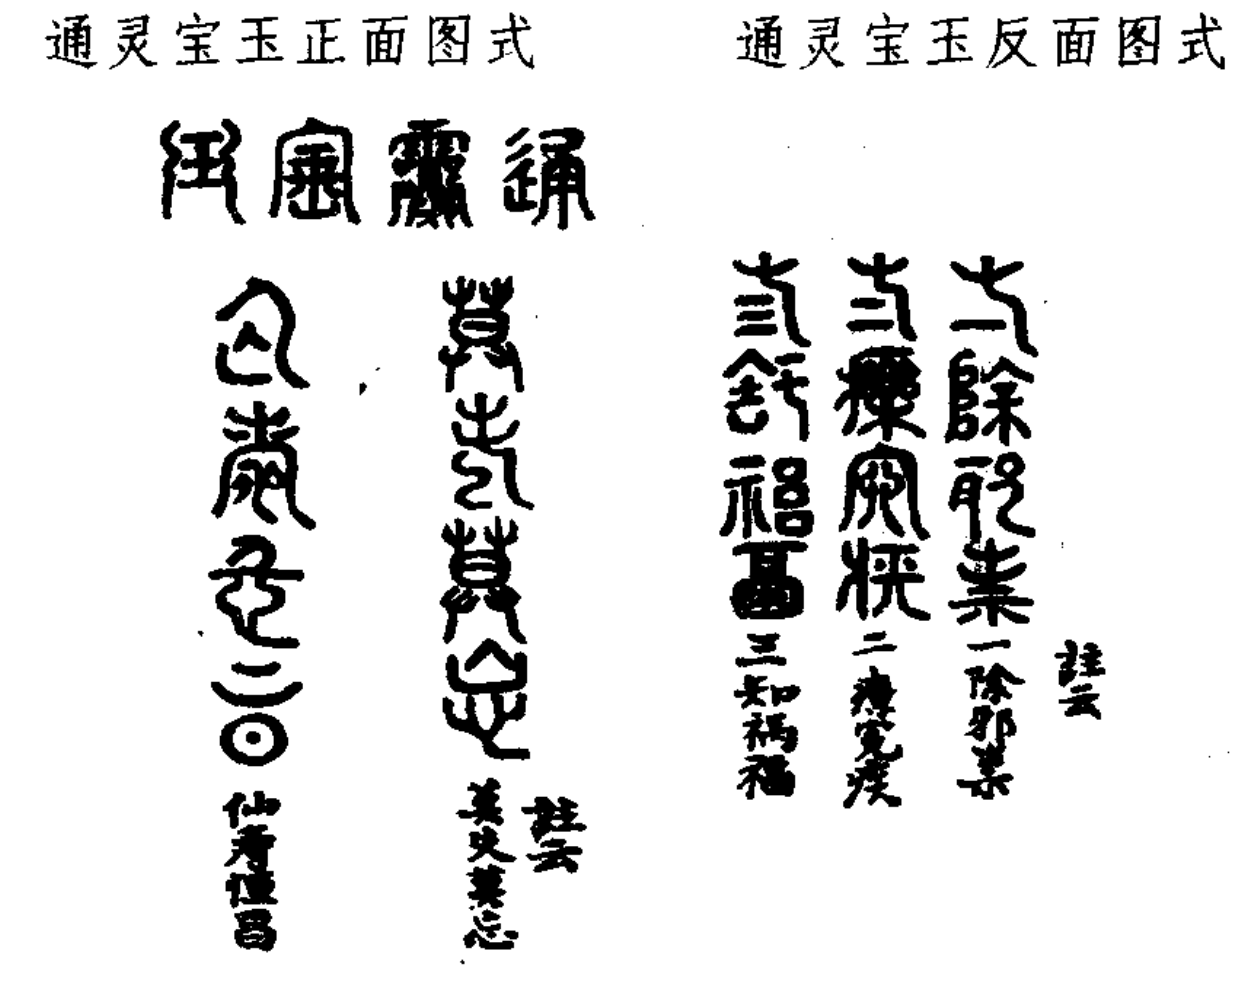
\includegraphics[scale=0.6]{picture/红楼梦1.PNG}
\end{figure}
\par 宝钗看毕,又从新翻过正面来细看,口内念道:“莫失莫忘,仙寿恒昌。”念了两遍,乃回头向莺儿笑道:“你不去倒茶,也在这里发呆作什么?”莺儿嘻嘻笑道:“我听这两句话,倒像和姑娘的项圈上的两句话是一对儿。”宝玉听了,忙笑道:“原来姐姐那项圈上也有八个字,我也赏鉴赏鉴。”宝钗道:“你别听他的话,没有什么字。”宝玉笑央:“好姐姐,你怎么瞧我的了呢。”宝钗被缠不过,因说道:“也是个人给了两句吉利话儿,所以錾上了,叫天天带着;不然,沉甸甸的有什么趣儿。”一面说,一面解了排扣,从里面大红袄上将那珠宝晶莹黄金灿烂的璎珞掏将出来。宝玉忙托了锁看时,果然一面有四个篆字,两面八字,共成两句吉谶\footnote{吉谶(chèn衬)——预示吉利的话。谶:预言。}。亦曾按式画下形相:
\begin{figure}[htb]
    \centering
    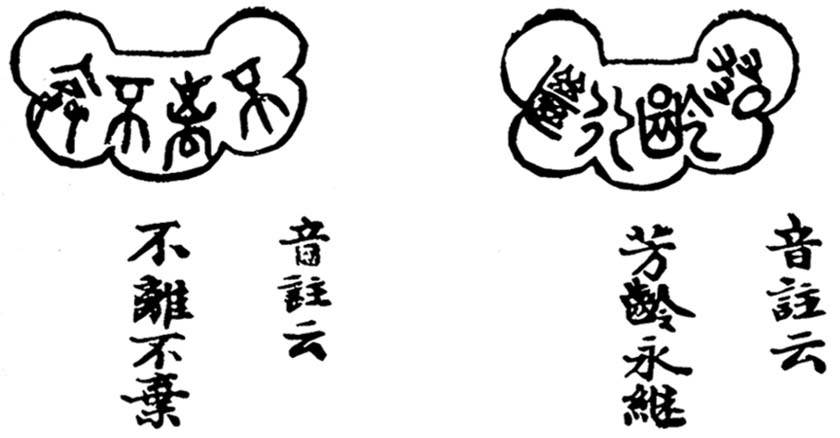
\includegraphics[scale=0.4]{picture/红楼梦2.jpeg}
\end{figure}
\par 宝玉看了,也念了两遍,又念自己的两遍,因笑问:“姐姐这八个字倒真与我的是一对。”莺儿笑道:“是个癞头和尚送的,他说必须錾在金器上——”宝钗不待说完,便嗔他不去倒茶,一面又问宝玉从那里来。
\par 宝玉此时与宝钗就近,只闻一阵阵凉森森甜丝丝的幽香,竟不知系何香气,遂问:“姐姐熏的是什么香?我竟从未闻见过这味儿。”宝钗笑道:“我最怕熏香,好好的衣服,熏的烟燎火气的。”宝玉道:“既如此,这是什么香?”宝钗想了一想,笑道:“是了,是我早起吃了丸药的香气。”宝玉笑道:“什么丸药这么好闻?好姐姐,给我一丸尝尝。”宝钗笑道:“又混闹了,一个药也是混吃的?”
\par 一语未了,忽听外面人说:“林姑娘来了。”话犹未了,林黛玉已摇摇的走了进来,一见了宝玉,便笑道:“嗳哟,我来的不巧了!”宝玉等忙起身笑让坐,宝钗因笑道:“这话怎么说?”黛玉笑道:“早知他来,我就不来了。”宝钗道:“我更不解这意。”黛玉笑道:“要来一群都来,要不来一个也不来;今儿他来了,明儿我再来,如此间错开了来着,岂不天天有人来了?也不至于太冷落,也不至于太热闹了。姐姐如何反不解这意思?”
\par 宝玉因见他外面罩着大红羽缎\footnote{羽缎——又称羽毛缎,一种毛织品,疏细者称羽纱,厚密者称羽缎,着水不湿,可御雨雪。}对衿褂子,因问:“下雪了么?”地下婆娘们道:“下了这半日雪珠儿了。”宝玉道:“取了我的斗篷来不曾?”黛玉便道:“是不是,我来了他就该去了。”宝玉笑道:“我多早晚儿说要去了?不过拿来预备着。”宝玉的奶母李嬷嬷因说道:“天又下雪,也好早晚的了,就在这里同姐姐妹妹一处顽顽罢。姨妈那里摆茶果子呢。我叫丫头去取了斗篷来,说给小幺儿们散了罢。”宝玉应允。李嬷嬷出去,命小厮们都各散去不提。
\par 这里薛姨妈已摆了几样细巧茶果来留他们吃茶。宝玉因夸前日在那府里珍大嫂子的好鹅掌鸭信\footnote{鸭信——鸭舌头,可制成名菜。信:舌头。}。薛姨妈听了,忙也把自己糟的取了些来与他尝。宝玉笑道:“这个须得就酒才好。”薛姨妈便令人去灌了最上等的酒来。李嬷嬷便上来道:“姨太太,酒倒罢了。”宝玉央道:“妈妈,我只喝一钟。”李嬷嬷道:“不中用!当着老太太、太太,那怕你吃一坛呢。想那日我眼错不见一会,不知是那一个没调教的,只图讨你的好儿,不管别人死活,给了你一口酒吃,葬送的我挨了两日骂。姨太太不知道,他性子又可恶,吃了酒更弄性。有一日老太太高兴了,又尽着他吃,什么日子又不许他吃,何苦我白赔在里面。”薛姨妈笑道:“老货,你只放心吃你的去。我也不许他吃多了。便是老太太问,有我呢。”一面令小丫鬟:“来,让你奶奶们去,也吃一杯搪搪雪气。”那李嬷嬷听如此说,只得和众人去吃些酒水。
\par 这里宝玉又说:“不必温暖了,我只爱吃冷的。”薛姨妈忙道:“这可使不得,吃了冷酒,写字手打飐儿\footnote{打飐儿——即打颤儿,发抖。}。”宝钗笑道:“宝兄弟,亏你每日家杂学旁收\footnote{杂学旁收——相对于应世举业的“正途”学问而言,即不去攻读《四书》《五经》时文八股而爱好诗词曲赋小说戏曲以至茶酒医药等闲杂学问。}的,难道就不知道酒性最热,若热吃下去,发散的就快;若冷吃下去,便凝结在内,以五脏去暖他,岂不受害?从此还不快不要吃那冷的了。”宝玉听这话有情理,便放下冷酒,命人暖来方饮。
\par 黛玉磕着瓜子儿,只抿着嘴笑。可巧黛玉的小丫鬟雪雁走来与黛玉送小手炉,黛玉因含笑问他:“谁叫你送来的?难为他费心,那里就冷死了我!”雪雁道:“紫鹃姐姐怕姑娘冷,使我送来的。”黛玉一面接了,抱在怀中,笑道:“也亏你倒听他的话。我平日和你说的,全当耳旁风;怎么他说了你就依,比圣旨还快些!”宝玉听这话,知是黛玉借此奚落他,也无回复之词,只嘻嘻的笑两声罢了。宝钗素知黛玉是如此惯了的,也不去睬他。薛姨妈因道:“你素日身子弱,禁不得冷的,他们记挂着你倒不好?”黛玉笑道:“姨妈不知道。幸亏是姨妈这里,倘或在别人家,人家岂不恼?好说就看的人家连个手炉也没有,巴巴的从家里送个来。不说丫鬟们太小心过馀,还只当我素日是这等轻狂惯了呢。”薛姨妈道:“你这个多心的,有这样想,我就没这样心。”
\par 说话时,宝玉已是三杯过去。李嬷嬷又上来拦阻。宝玉正在心甜意洽之时,和宝黛姊妹说说笑笑的,那肯不吃。宝玉只得屈意央告:“好妈妈,我再吃两钟就不吃了。”李嬷嬷道:“你可仔细老爷今儿在家,隄防问你的书!”宝玉听了这话,便心中大不自在,慢慢的放下酒,垂了头。黛玉先忙的说:“别扫大家的兴!舅舅若叫你,只说姨妈留着呢。这个妈妈,他吃了酒,又拿我们来醒脾\footnote{醒脾——即开胃;可引申为开心。本中医术语,是指一种治疗脾气虚寒、运化无力的方法。}了!”一面悄推宝玉,使他赌气;一面悄悄的咕哝说:“别理那老货,咱们只管乐咱们的。”那李嬷嬷不知黛玉的意思,因说道:“林姐儿,你不要助着他了。你倒劝劝他,只怕他还听些。”林黛玉冷笑道:“我为什么助他?我也不犯着劝他。你这妈妈太小心了,往常老太太又给他酒吃,如今在姨妈这里多吃一口,料也不妨事。必定姨妈这里是外人,不当在这里的也未可定。”李嬷嬷听了,又是急,又是笑,说道:“真真这林姐儿,说出一句话来,比刀子还尖。你——这算了什么。”宝钗也忍不住笑着,把黛玉腮上一拧,说道:“真真这个颦丫头的一张嘴,叫人恨又不是,喜欢又不是。”薛姨妈一面又说:“别怕,别怕,我的儿!来这里没好的你吃,别把这点子东西唬的存在心里,倒叫我不安。只管放心吃,都有我呢。越发吃了晚饭去,便醉了,就跟着我睡罢。”因命:“再烫热酒来!姨妈陪你吃两杯,可就吃饭罢。”宝玉听了,方又鼓起兴来。
\par 李嬷嬷因吩咐小丫头子们:“你们在这里小心着,我家里换了衣服就来,悄悄的回姨太太,别由着他,多给他吃。”说着便家去了。这里虽还有三两个婆子,都是不关痛痒的,见李嬷嬷走了,也都悄悄去寻方便去了。只剩了两个小丫头子,乐得讨宝玉的欢喜。幸而薛姨妈千哄万哄的,只容他吃了几杯,就忙收过了。作酸笋鸡皮汤,宝玉痛喝了两碗,吃了半碗碧粳粥。一时薛林二人也吃完了饭,又酽酽的沏上茶来大家吃了。薛姨妈方放了心。雪雁等三四个丫头已吃了饭,进来伺候。黛玉因问宝玉道:“你走不走?”宝玉乜斜\footnote{乜(miē咩)斜——眯着眼睛,斜眼看人。}倦眼道:“你要走,我和你一同走。”黛玉听说,遂起身道:“咱们来了这一日,也该回去了。还不知那边怎么找咱们呢。”说着,二人便告辞。
\par 小丫头忙捧过斗笠来,宝玉便把头略低一低,命他戴上。那丫头便将着大红猩毡斗笠一抖,才往宝玉头上一合,宝玉便说:“罢,罢!好蠢东西,你也轻些儿!难道没见过别人戴过的?让我自己戴罢。”黛玉站在炕沿上道:“罗唆什么,过来,我瞧瞧罢。”宝玉忙就近前来。黛玉用手整理,轻轻笼住束发冠,将笠沿掖在抹额之上,将那一颗核桃大的绛绒簪缨扶起,颤巍巍露于笠外。整理已毕,端相了端相,说道:“好了,披上斗篷罢。”宝玉听了,方接了斗篷披上。薛姨妈忙道:“跟你们的妈妈都还没来呢,且略等等不迟。”宝玉道:“我们倒去等他们,有丫头们跟着也够了。”薛姨妈不放心,到底命两个妇女跟随他兄妹方罢。他二人道了扰,一径回至贾母房中。
\par 贾母尚未用晚饭,知是薛姨妈处来,更加欢喜。因见宝玉吃了酒,遂命他自回房去歇着,不许再出来了。因命人好生看侍着。忽想起跟宝玉的人来,遂问众人:“李奶子怎么不见?”众人不敢直说家去了,只说:“才进来的,想有事才去了。”宝玉踉跄回头道:“他比老太太还受用呢,问他作什么!没有他只怕我还多活两日。”一面说,一面来至自己的卧室。只见笔墨在案,晴雯先接出来,笑说道:“好,好,耍\footnote{耍——戏弄之意。}我研了那些墨,早起高兴,只写了三个字,丢下笔就走了,哄的我们等了一日。快来与我写完这些墨才罢!”宝玉忽然想起早起的事来,因笑道:“我写的那三个字在那里呢?”晴雯笑道:“这个人可醉了。你头里过那府里去,嘱咐贴在这门斗上,这会子又这么问。我生怕别人贴坏了,我亲自爬高上梯的贴上,这会子还冻的手僵冷的呢。”宝玉听了,笑道:“我忘了。你的手冷,我替你渥\footnote{渥(wò沃)——覆盖裹藏某物,借以保暖或使之变暖,叫“渥”。}着。”说着便伸手携了晴雯的手,同仰首看门斗上新书的三个字。
\par 一时黛玉来了,宝玉笑道:“好妹妹,你别撒谎,你看这三个字那一个好?”黛玉仰头看里间门斗上,新贴了三个字,写着“绛云轩”。黛玉笑道:“个个都好。怎么写的这们好了?明儿也与我写一个匾。”宝玉嘻嘻的笑道:“又哄我呢。”说着又问:“袭人姐姐呢?”晴雯向里间炕上努嘴。宝玉一看,只见袭人和衣睡着在那里。宝玉笑道:“好,太渥早了些。”因又问晴雯道:“今儿我在那府里吃早饭,有一碟子豆腐皮的包子,我想着你爱吃,和珍大奶奶说了,只说我留着晚上吃,叫人送过来的,你可吃了?”晴雯道:“快别提。一送了来,我知道是我的,偏我才吃了饭,就放在那里。后来李奶奶来了看见,说:‘宝玉未必吃了,拿来给我孙子吃去罢。’他就叫人拿了家去了。”接着茜雪捧上茶来。宝玉因让“林妹妹吃茶。”众人笑说:“林妹妹早走了,还让呢。”
\par 宝玉吃了半碗茶,忽又想起早起的茶来,因问茜雪道:“早起沏了一碗枫露茶,我说过,那茶是三四次后才出色的,这会子怎么又沏了这个来?”茜雪道:“我原是留着的,那会子李奶奶来了,他要尝尝,就给他吃了。”宝玉听了,将手中的茶杯只顺手往地下一掷,豁啷一声,打了个粉碎,泼了茜雪一裙子的茶。又跳起来问着茜雪道:“他是你那一门子的奶奶,你们这么孝敬他?不过是仗着我小时候吃过他几日奶罢了。如今逞的他比祖宗还大了。如今我又吃不着奶了,白白的养着祖宗作什么!撵了出去,大家干净!”说着便要去立刻回贾母,撵他乳母。
\par 原来袭人实未睡着,不过故意装睡,引宝玉来怄\footnote{怄(òu沤)——这里是撩拨逗弄、厮缠、磨人的意思。}他顽耍。先闻得说字问包子等事,也还可不必起来;后来摔了茶钟,动了气,遂连忙起来解释劝阻。早有贾母遣人来问是怎么了。袭人忙道:“我才倒茶来,被雪滑倒了,失手砸了钟子。”一面又安慰宝玉道:“你立意要撵他,也好,我们也都愿意出去,不如趁势连我们一齐撵了。我们也好,你也不愁再有好的来服侍你。”宝玉听了这话,方无了言语,被袭人等扶至炕上,脱换了衣服。不知宝玉口内还说些什么,只觉口齿缠绵,眼眉愈加饧涩,忙服侍他睡下。袭人伸手从他项上摘下那通灵玉来,用自己的手帕包好,塞在褥下,次日带时便冰不着脖子。那宝玉就枕便睡着了。彼时李嬷嬷等已进来了,听见醉了,不敢前来再加触犯,只悄悄的打听睡了,方放心散去。
\par 次日醒来,就有人回:“那边小蓉大爷带了秦相公来拜。”宝玉忙接了出去,领了拜见贾母。贾母见秦钟形容标致,举止温柔,堪陪宝玉读书,心中十分欢喜,便留茶留饭,又命人带去见王夫人等。众人因素爱秦氏,今见了秦钟是这般人品,也都欢喜,临去时都有表礼。贾母又与了一个荷包\footnote{荷包——用以装药品、香料等细小物品的扁圆形绣花小袋。}并一个金魁星\footnote{金魁星——黄金铸成的魁星神像,有祝颂功名顺利的意思。魁星:本作奎星,北斗第一星,汉代纬书《孝经援神契》有“奎主文章”之说,后遂以此星为掌文运之神。},取“文星和合\footnote{文星和合——“文星”又称文昌星、文曲星,星相家以其为吉星、主文运、保功名。“和合”与荷包谐音,且为中国民间所奉喜庆吉祥之神,本祀万回,清代雍正年间封天台僧人寒山、拾得为“和合二仙”。}”之意。又嘱咐他道:“你家住的远,或有一时寒热饥饱不便,只管住在这里,不必限定了。只和你宝叔在一处,别跟着那些不长进的东西们学。”秦钟一一的答应,回去禀知。
\par 他父亲秦业现任营缮郎\footnote{营缮郎——官名。明清时工部有营缮司,设郎中、员外郎等职。},年近七十,夫人早亡。因当年无儿女,便向养生堂\footnote{养生堂——又叫育婴堂。一种收养弃婴的慈善机构。}抱了一个儿子并一个女儿。谁知儿子又死了,只剩女儿,小名唤可儿,长大时,生的形容袅娜,性格风流。因素与贾家有些瓜葛,故结了亲,许与贾蓉为妻。那秦业至五旬之上方得了秦钟。因去岁业师亡故,未暇延请高明之士,只得暂时在家温习旧课。正思要和亲家去商议送往他家塾中,暂且不致荒废,可巧遇见了宝玉这个机会。又知贾家塾中现今司塾的是贾代儒,乃当今之老儒,秦钟此去,学业料必进益,成名可望,因此十分喜悦。只是宦囊羞涩\footnote{宦囊羞涩——意谓做官者手头拮据。语本“阮囊羞涩”,见《韵府群玉·阳韵》。},那贾家上上下下都是一双富贵眼睛,贽见礼\footnote{贽(zhì至)见礼——旧时学生拜见老师时所送的礼,封套上要写“贽敬”。}必须丰厚,\footnote{“贽见礼必须丰厚”七字,据戚序、蒙府本补。}容易\footnote{容易——轻易。}拿不出来,又恐误了儿子的终身大事,说不得东拚西凑的恭恭敬敬封了二十四两贽见礼,亲自带了秦钟,来代儒家拜见了。然后听宝玉上学之日,好一同入塾。正是:
\refdocument{
    \par 早知日后闲争气,岂肯今朝错读书。
}




